%Dokumentenklasse "scrbook" - Erweitert um den Verweis auf die Verzeichnisse und Texteigenschaften
\documentclass[chapterprefix=true, 10pt, a4paper, oneside, parskip=half, listof=totoc, bibliography=totoc, numbers=noendperiod]{scrbook}

% Ränder (Standard bottom ca. 52mm anbzüglich von ca. 4mm für die nach oben rechts gewanderte Seitenzahl)
%Anpassung der Seitenränder
\usepackage[bottom=32mm,left=25mm,right=25mm]{geometry}

% Ränder bei Bedarf zeigen
%\usepackage{showframe}

%Tweaks für scrbook
\usepackage{scrhack}

%Blindtext
\usepackage{blindtext}

%Erlaubt unteranderem Umbrücke captions
\usepackage{caption}

%Stichwortverzeichnis
\usepackage{imakeidx}

%Kompakte Listen
\usepackage{paralist}

%Zitate besser formatieren und darstellen
\usepackage{epigraph}

%Glossar + Stichworverzeichnis
\usepackage[toc, acronym]{glossaries} % Akronyme werden als eigene Liste aufgeführt
\glsenablehyper

%Anpassung von Kopf- und Fußzeile
%beinflusst die erste Seite des Kapitels
\usepackage[automark,headsepline]{scrlayer-scrpage}
\automark{chapter}
\ihead{\leftmark}
\chead{}
\ohead{\thepage}
\ifoot*{}
\cfoot[\thepage]{}
\cfoot*{}
\ofoot*{}
\pagestyle{scrheadings}

%Auskommentieren für die Verkleinerung des vertikalen Abstandes eines neuen Kapitels
%\renewcommand*{\chapterheadstartvskip}{\vspace*{.25\baselineskip}}

%Zeilenabstand 1,5
\usepackage[onehalfspacing]{setspace}

%Verbesserte Darstellung der Buchstaben zueinander
\usepackage[stretch=10]{microtype}

%Deutsche Bezeichnungen für angezeigte Namen (z.B. Innhaltsverzeichnis etc.)
\usepackage[ngerman]{babel}

%Unterstützung von Umlauten und anderen Sonderzeichen (UTF-8)
\usepackage{lmodern}
\usepackage[utf8]{luainputenc}
\usepackage[T1]{fontenc}

%Einfachere Zitate
\usepackage{epigraph}

%Verwendung von Akronymen
\usepackage[printonlyused]{acronym}

%Unterstützung der H positionierung (keine automatische Verschiebung eingefügter Elemente)
\usepackage{float} 

%Erlaubt Umbrüche innerhalb von Tabellen
\usepackage{tabularx}

%Erlaubt Seitenumbrüche mit Tabellen
\usepackage{longtable}

%Erlaubt die Darstellung von Sourcecode mit Highlighting
\usepackage{listings}

%Definierung eigener Farben bei nutzung eines selbst vergebene Namens
\usepackage[table,xcdraw]{xcolor}

%Vektorgrafiken tikz
\usepackage{tikz}

%Grafiken (wie jpg, png, etc.)
\usepackage{graphicx}

%Grafiken von Text umlaufen lassen
\usepackage{wrapfig}

%Grafik bestehend aus mehreren Grafiken
\usepackage{subfigure}

%Ermöglicht Verknüpfungen innerhalb des Dokumentes (e.g. for PDF), Links werden durch "hidelink" nicht explizit hervorgehoben
\usepackage[hidelinks,ngerman]{hyperref}

%Einbindung und Verwaltung von Literaturverzeichnissen
\usepackage{csquotes} %wird von biber benötigt
\usepackage[style=alphabetic, backend=biber, bibencoding=utf8]{biblatex}
\addbibresource{references/references.bib}

%enable the macro \mathbb
\usepackage{amssymb}
\usepackage{amsmath}

%-------------------------------Zusätzliche Anpassungen und Modifikationen--------------------------------------------%

%Anpassung der Überschriften
\addtokomafont{disposition}{\rmfamily}

%Zusätzliche Farben
\definecolor{Ao}{rgb}{0.0, 0.39, 0.0}
\definecolor{antiquefuchsia}{rgb}{0.57, 0.36, 0.51}
\definecolor{bostonuniversityred}{rgb}{0.8, 0.0, 0.0}

% Padding für images innerhalb von longtables
\usepackage{verbatimbox}
\newcommand\Includegraphics[2][]{\addvbuffer[5pt 0pt]{\includegraphics[#1]{#2}}}

%Umbenennungen
\renewcommand{\lstlistlistingname}{Source Code Content}

%Pluszeichen in der Reference beim zitieren ausblenden
\renewcommand*{\labelalphaothers}{}

%Anpassugen zur Quelltextdarstellung, kann bei Bedarf überschrieben werden (z.B. wenn unterschiedliche Sprachen zum Einsatz kommen)
\renewcommand{\lstlistingname}{Code snippet}
\lstset{
	language=python,
	numbers=left,
	columns=fullflexible,
	aboveskip=5pt,
	belowskip=10pt,
	basicstyle=\small\ttfamily,
	backgroundcolor=\color{black!5},
	commentstyle=\color{black},
	morecomment=[s]{.s}{hape}, % workaround to exclude ".shape"
	keywordstyle=\color{antiquefuchsia},
	otherkeywords={self, else},
	emphstyle=\color{bostonuniversityred},
	emph={shape,units,name,filters,kernel_size,activation,padding,kernel_initializer,kernel_regularizer,bias_initializer,inputs,outputs,mode,distribution,minval,val, callback_args, low, high, limit, window_length, size, mu, theta, sigma},
	stringstyle=\color{Ao},
	showspaces=false,
	showstringspaces=false,
	showtabs=false,
	xleftmargin=16pt,
	xrightmargin=0pt,
	framesep=5pt,
	framerule=1pt,
	frame=leftline,
	rulecolor=\color{black},
	tabsize=2,
	breaklines=true,
	breakatwhitespace=true
}

%Anpassungen für das Abkürzungsverzeichnis
\newglossarystyle{dottedlocations}{%
	\glossarystyle{list}%
	\renewcommand*{\glossaryentryfield}[5]{%
		\item[\glsentryitem{##1}\glstarget{##1}{##2}] \emph{##3}%
		\unskip\leaders\hbox to 2.9mm{\hss.}\hfill##5}%
	\renewcommand*{\glsgroupskip}{}%
}
\usepackage{tabu}
\usepackage{makecell}
\usepackage{flafter} 
\usepackage{pdfpages}
% Titles Config - CHOOSE ONE section for title format

%% Used for titleGraduation Bachelor
%% Based on https://ai-bachelor.htw-berlin.de/files/Stg/AI/richtlinie_ba-arbeit_ai_06_02_13.pdf
\makeatletter

\newcommand*{\gradeType}[1]{\gdef\@gradeType{#1}}
\newcommand*{\firstExaminer}[1]{\gdef\@firstExaminer{#1}}
\newcommand*{\secondExaminer}[1]{\gdef\@secondExaminer{#1}}
\newcommand*{\matrikelnr}[1]{\gdef\@matrikelnr{#1}}
\newcommand*{\submitDate}[1]{\gdef\@submitDate{#1}}

\renewcommand*{\maketitle}{
	\begin{titlepage}
		\newgeometry{left=2.5cm,right=2.5cm,top=2.5cm,bottom=2.5cm}
		\begin{figure}[H]
			\centering
			
\includegraphics[width=0.5\textwidth]{resources/htw/logo}
		\end{figure}
		\begin{center}
			\vfill
			{\Large \@title\par}
			\vskip 0.5cm
			{\large \bfseries Abschlussarbeit\par}
			\vskip 0.5cm
			{\large zur Erlangung des akademischen Grades\vskip 0.5cm \bfseries \@gradeType}
			\vskip 0.5cm
			{\large an der}
			\vskip 0.5cm
			{\large Hochschule für Technik und Wirtschaft Berlin}
			\vskip 0.0cm
			{\large Fachbereich IV (Informatik, Kommunikation und Wirtschaft) }
			\vskip 0.0cm
			{\large Studiengang Angewandte Informatik}
			\vfill
			\begin{flushleft}
				\begin{tabular}[t]{rl}
					1. Prüfer: &\@firstExaminer\\
					2. Prüfer: & \@secondExaminer\\
					\\
					Eingereicht von: &\@author\\
					Immatrikulationsnummer: & \@matrikelnr\\
					Eingereicht am: & \@submitDate
				\end{tabular}
			\end{flushleft}
		\end{center}
		\restoregeometry
	\end{titlepage}
}
\makeatother
\gradeType{Bachelor of Science (B.Sc.)}
\secondExaminer{Dipl. Sport-ing. Andreas Geiger}

% Titles Config End

% Used by all titles
\title{Entwurf und Implementierung eines Augmented Reality Systems für Produkt-Design-Feedback durch den Endkunden }
\author{Ali Bektas}
\matrikelnr{s0559003}
\submitDate{07.09.2019}
\firstExaminer{Prof. Dr. Thomas Jung}
% End Titles

\makeindex[title=Index, options=-s indexstyle.ist, intoc]
\indexsetup{level=\chapter*,toclevel=chapter}

\makenoidxglossaries
\loadglsentries{glossary_and_acronyms.tex}
\setacronymstyle{long-short}
\begin{document}

\pagenumbering{alph} % fix for same identifier warning, character is not show in title
\maketitle

\pagenumbering{Roman}
\chapter*{Vorwort}
TODO \clearpage  
\chapter*{Kurzbeschreibung}
TODO
\\
\\
\textbf{Schlagworte:} Mixed Reality, Gemischte Realität, Augmented Reality, Ergänzte Realität, Microsoft Hololens, Open Innovation, Design Feedback \clearpage

\tableofcontents \newpage

\pagenumbering{arabic}
\chapter{Einleitung}

\section{Motivation}

[...]

\section{Zielsetzung}

Das Ziel dieser Arbeit ist es, ein System zu konzipieren und einen Prototypen zu entwickeln, welches dem Anwender ermöglicht, Feedback an Produkten
abzugeben. 

Das zu konzipierende System soll zum einen Anwendungsszenarien unterstützen, in welcher Nutzer Feedbacks zu Produkten abgeben können, 
zum anderen soll Nutzern ermöglicht werden, diese Feedbacks auf den Produkten zu explorieren. 
Diese Kommunikation soll eine Kollaboration von mehreren Nutzern, mit dem Produkt im Mittelpunkt, ermöglichen und zum Ziel haben, die Qualität der 
Produkte und die damit verbundene Kundenzufriedenheit zu verbessern.

Die prototypische Implementierung soll sich auf die Erstellung, Bearbeitung und Löschung von Feedbacks eingrenzen. Die Feedbacks sollen auf dem physischen 
Produkt in Form von Annotationen dargestellt, und in einer im Web übertragbaren Format gespeichert werden. Dies soll den Zugriff auf diese Daten 
(z. Bsp. für die Überführung in ein Anforderungsmanagement System) über eine Schnittstelle realisierbar machen.  

Nach der Implementierung des Prototypen, soll die Usability für die Erstellung, Änderung und Löschung von Feedbacks an einem durch 
eine Usability Studie evaluiert werden. 

\section{Vorgehensweise und Aufbau der Arbeit}

Zunächst werden im Kapitel \ref{CapterFundamentals} Grundalgen näher gebracht, die für das Verständnis dieser Arbeit benötigt werden. Anschließend wird 
im Kapitel 3 ein Überblick über den Stand der Technik im Bereich der Augmented Reality Technologien gegeben sowie Paradigmen für die Selektion in 3D Benutzeroberflächen, 
für die Anwendung auf mobilen Endgeräten wie Smartphones oder Tabletts analysiert.  
 
Im Kapitel 4 wird die Konzeption des Systems beschrieben. Zunächst wird der Nutzungskontext des zu konzipierenden Systems analysiert und 
anschließend der Verlauf eines Kreativ Workshops beschrieben, welcher als Grundlage für die Anforderungsanalyse diente. Abschließend werden in diesem Kapitel 
die Anforderungen an den zu entwickelnden Prototypen beschrieben und ein Papierprototyp vorgestellt. 

Basierend auf den, in den vorangegangen zwei Kapitel erarbeiteten Konzeption und den dort definierten Anforderungen, wird im Kapitel 5 der Verlauf für die 
Umsetzung des digitalen Prototypen beschrieben.      

Im Kapitel 6 wird zunächst die Planung der durchzuführenden Nutzerstudie beschrieben. Dies beinhaltet die Festlegung des Studiendesigns sowie die Planung der Prozedur und die des Ablaufplans. 
Anschließend wird die Durchführung der Studie beschreiben sowie die Ergebnisse der erhobenen Daten vorgestellt. Zuletzt werden Folgerungen zu den aus der Studie erhobenen Daten erläutert und ein Fazit gezogen.

Abschließend wird im Kapitel 7 ein Fazit gezogen und die Arbeit zusammengefasst. Es wird in einer kritischen Rückblick erläutert [... weis noch nicht wie ich das hier beschreiben soll. Im Sinne
von was hätte Rückblickend besser gemacht werden können. Wo wurden Fehler gemacht. Ohne zu sehr nach hätte, hätte Fahrradkette zu klingen ...]. 
Zuletzt werden mögliche Erweiterungsmöglichkeiten der Anwendung beschrieben.  \clearpage
\chapter{Grundlagen} \label{CapterFundamentals}

Dieses Kapitel gibt einen Überblick über die in dieser Arbeit verwendete Terminologien und führt Grundlagen zu Technologien und Techniken ein welche die Basis für dieser Arbeit bilden. 

Nach Erläuterung Definition von Augmented Reality, werden unterschiedliche Ansätze für die Objekterkennung und Verfolgung vorgestellt.  
Diese sind ein essenzieller Bestandteil der Augmented Reality Technologie. Es wird die Definition von Situated Visualization erläutert 
und Visualisierungstechniken für die Darstellung von Daten im Kontext zur physischen Welt (z. Bsp. Gegenstände, Person, Aufgabe) nahe gebracht. 
Abschließend wird die Definition von Usability erläutert und ein Einblick in Usability Engineering gegeben, welches eine etablierte Vorgehensweise für die 
Gestaltung und Entwicklung von Systemen mit hohen Usability Anforderungen ist. 

\section{Augmented Reality}

%Definition und Begriffseingrenzung  von AR
Augmented Reality (zu dt. Erweiterte Realität, kurz AR) steht für die Überlagerung der realen Welt mit digitalen Informationen. \cite{Azuma.1997,DieterSchmalstieg2016} Im Gegensatz zu, virtuellen Realität, wo Benutzer vollständig in virtuelle Umgebungen eintauchen,
ist das Ziel von AR, Informationen direkt in die physische Umgebung des Benutzers einzufügen. So soll der Eindruck entstehen, dass diese Informationen Teil der realen Welt sind. \footnote{Nach Definition von Azuma  müssen Informationen hierbei nicht nur auf visuelle Informationen beschränkt sein, 
sondern können auch auditive, haptische, gustative (Geschmack) oder auch olfaktorische (Geruch) umfassen.} \cite{Azuma.1997} Während in VR Benutzer von der äußeren Umgebung nichts mitbekommen, wird in AR die reale Umgebung des Benutzers, mit virtuellen 
Objekten überlagert. Azuma beschreibt in \cite{Azuma.1997}, folgende Charakteristiken für Augmented Reality: 

\begin{enumerate}
	\item Kombinieren reale und virtuelle Welt (Combines real and virtual).
	\item Ermöglichen Interaktionen in Echtzeit. (Interactive in real time)
	\item Informationen (reale und virtuelle) haben einen Bezug im dreidimensionalen Raum. (Registered in 3-D)
\end{enumerate}

Diese Charakteristiken helfen dabei Augmented Reality besser zu verstehen und technologisch einzuordnen. \cite{Azuma.1997} Filme, wie z. Bsp. ``Jurassic Park``, in welchen virtuelle Objekte in die reale Szene eingefügt werden, erwecken zwar den Eindruck, dass diese Objekte, Teil der realen Szene sind, jedoch kann mit diesen Objekten nicht in Echtzeit interagiert werden. \cite{Tonnis2010} In Filmen werden die virtuellen Objekte in eine zuvor aufgezeichnete Aufnahme eingefügt. 
In der AR Technologie werden hingegen virtuelle Objekte live in ein Video eingefügt. Dies bedeutet, dass in  Filmen für das Einfügen von digitalen Informationen in die reale Szene beliebig große Zeitspanne zur Verfügung steht. 
In AR muss dies in wenigen Millisekunden geschehen. Die neue Position und Ausrichtung des virtuellen Objektes in live Szene muss innerhalb einer Zeitspanne von zwei Frames bestimmt werden.

Ein anderes Beispiel für AR ist in Live-Ansichten von Digitalkameras zu finden, welche das aufzunehmende Bild als Vorschau anzeigen. Oft blenden Digitalkameras Informationen zu den aktuellen Einstellungen der Kamera sowie den 
Ladezustand der Batterie im Vorschaubild ein (Siehe Abbildung \ref{img:ar_camera_example}). Diese Informationen überlagern zwar die reale Szene, haben jedoch keinen Bezug zum dreidimensionalen Raum. 
Der elektronische Sucher hingegen welches Objekte (z. Bsp. Gesichter) erkennt und in einem virtuellen Rahmen einrahmt, hat ein Bezug zu den Objekten im 3D Raum. 
Zudem sind Interaktionen in Echtzeit möglich. Bewegt sich das vom virtuellen Rahmen, eingerahmte reale Objekt, oder die Kamera selbst, verändert sich auch die Position des virtuellen Objektes. 

\begin{figure}
	\centering
	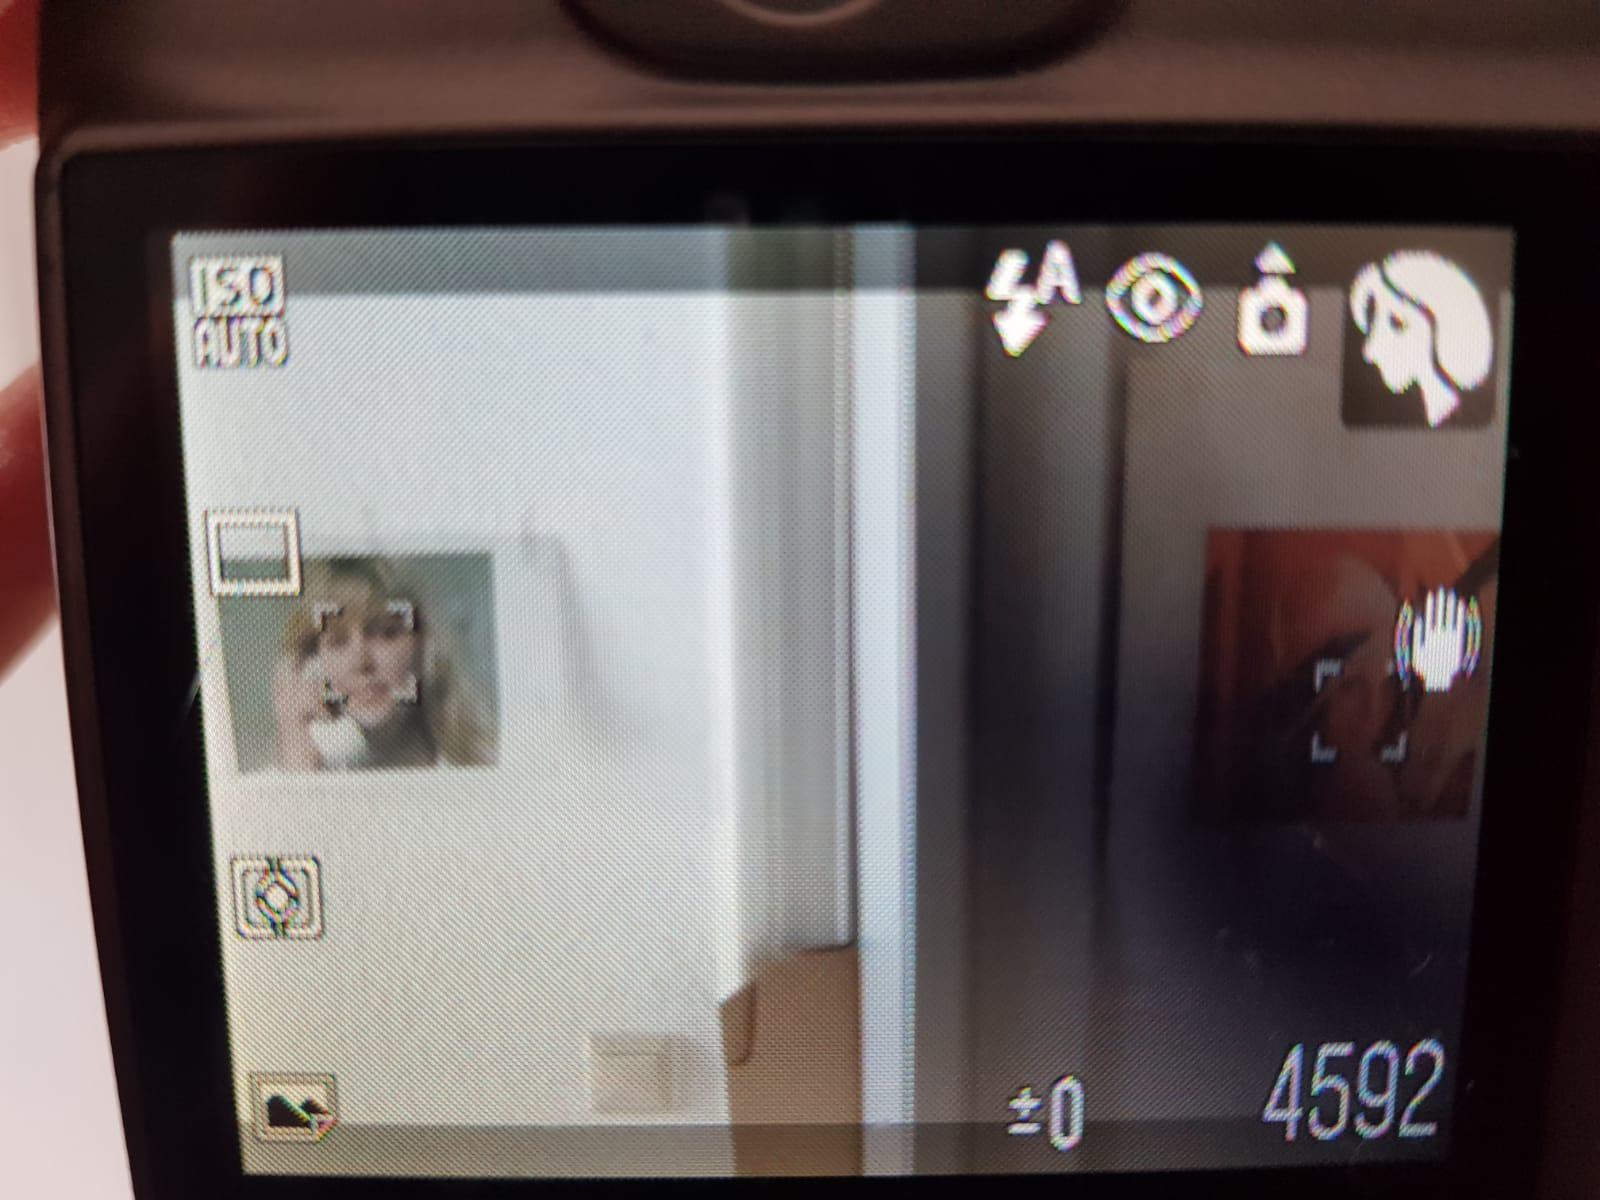
\includegraphics[width=0.50\textwidth]{resources/fundamentals/example_camera_screen_ar}
	\caption{Beispielhafte Darstellung eines Digitalkamera-Display mit eingeblendeten digitalen zusätzlichen Informationen. Quelle: Eigene Darstellung}
	\label{img:ar_camera_example}
\end{figure}

% Motivation
\cite{Azuma.1997} Durch das Kombinieren von virtueller und physischer Welt, erweitert Augumented Reality die Wahrnehmung des Menschen. Die Motivation von AR ist, dem Menschen durch das Einfügen
von digitalen Informationen in die physische Welt, Hinweise zu geben und Details zu zeigen, die sonst nicht unmittelbar wahrnehmen könnte. Diese Informationen sollen den Menschen 
bei der Verrichtung ihrer Aufgaben in der physischen Welt unterstützen.

% Anwendungsfelder von AR % Besonders passend für diese Arbeit sind Annotationen und Warung und Reperatur. Da diese sich besonders mit Interaktionen an Realen Objekten, meist Produkte befassen.
Azuma fasst in \cite{Azuma.1997}, Forschungen zu AR in sechs Anwendungsgebiete zusammen: Zur Visualisierung von Medizindaten, in der Wartung 
und Instandsetzung, Annotationen, für die Wegfindung in der Robotik und für die Navigation von Militärflugzeugen. Beispielsweise können Annotationen 
verwendet werden, um Informationen über den Inhalt von Regalen einzublenden, während ein Nutzer durch eine Bibliothek läuft und nach bestimmten Büchern sucht. % Füge hier vielleicht noch ein Beispiel dazu ein % Füge hier Verweis auf ein Artike als Fußnotel hinzu
Auch können Annotationen in AR verwendet werden, um einzelne Bauelemente an komplexen Bauteilteilen zu identifizieren und Informationen über diese zu visualisieren. 
In der Wartung und Instandsetzung können Augemented Reality Anwendungen dabei helfen, Instruktionen an komplexen Maschinen und Anlagen zu visualisieren, welche sonst in 
Form von Text und Bildern vorliegen. So können virtuelle Replikate über die physischen Modelle gelegt und, zum Beispiel, Schritt für Schritt Anleitungen direkt am physischen Produkt visualisiert werden. 
Durch Animationen können diese Anleitungen präziser gestaltet werden und zum Beispiel auch Informationen über die Richtung geben. 

Diese Systeme können heute zum Beispiel Unterunternehmen dabei helfen, besser mit ihren Kunden zu kooperieren. In Kombination mit der Technologie Internet of Things (IOT) können Unternehmen,
zustands-bezogene Informationen zu Ihren Systemen bei Endkunden abrufen und proaktiv Ihre Kunden auf notwendige Wartungen am physischen System, aufmerksam machen. Wartungsanleitungen können dann direkt 
an den Analgen angezeigt werden, sodass Endkunden diese selbständig durchführen können.\footnote{Fallstudie zur Anwendung von AR in Wartung von Industrieanlagen: https://www.ptc.com/-/media/Files/PDFs/Case-Studies/Howden-vuforia-studio-case-study-Feb-2019.pdf?la=en\&hash=6342841E1B6470C1F313295427398606 [letzter Zugriff: 25.06.2019]}

%Grundlegende Techniken
\cite[S.~32]{Tonnis2010} Für die Überlagerung der realen Welt mit virtuellen Objekten eignen sich nach heutigem Stand der Technik zwei Display Techniken, nämlich Optical See-Through und Video See-Through. 
Bei Optical See-Through kann der Nutzer direkt in die reale Welt blicken, wobei Computer generierte Bilder auf ein halbdurchlässiges Spiegel eingeblendet werden (dieses wird als Combiner bezeichnet).
Diese Technik hat den Vorteil, dass der Nutzer einen direkten Blick auf die reale Welt hat. Der Nachteil ist jedoch, dass die reale Welt nicht zeitgleich mit virtuellen Objekten überlagert werden kann. 
Dadurch, dass die Berechnung der Positionsbestimmung und das Rendern der virtuellen Objekte Zeit in Anspruch nimmt, werden diese mit einer kleinen Verzögerung angezeigt. Dies kann, auch 
wenn es sich nur um einige Millisekunden handelt, zu einem so genannten Schwimmeffekt führen (en. Lag). Mit der See Through Display Technik, wird die reale Welt dem Nutzer als ein Video 
angezeigt und mit virtuellen Objekten überlagert. Der Vorteil dieser Technik liegt darin, dass die Darstellung der realen Welt um die Zeit verzögert werden kann, die benötigt wird, um die virtuellen Objekte 
richtig zu positionieren und rendern. Dadurch werden die Nachteile der Optical-See-Through Technik kompensiert. Dass die reale Welt dem Nutzer verzögert angezeigt wird bringt jedoch den Nachteil, 
dass Positionsänderungen von physischen im realen Welt befindenden Objekten oder die Änderung der Perspektive, falls sich der Nutzer selbst bewegt, verzögert angezeigt werden. Zudem wird mit 
dieser Technik je nach Auflösung der Kamera die reale Welt mit verringerter Qualität angezeigt.

\section{Objekterkennung und- Verfolgung}

% Definition von Objekterkennung und Verfolgung

% Geschichte und Entwicklung

\subsection{Markerbasiertes Tracking}

% Begriffserklärung von Marker Trakting

% Anwendungsfelder von Marker Traking

\subsection{Markerloses Tracking}

% Begriffserklärung von Markerlosen Traking 

% Anwendungsfelder von Markerlosen Traking


\section{Situated Visualization}
\subsection{(Situated Visualization) - Definition}

Das zu konzipierende System soll durch den Einsatz von Augmented Reality, die Abgabe von Feedbacks zu Produkten und deren Darstellung auf den Produkten bzw. Produktteilen ermöglichen. 
Als eine besondere Form von Visualisierung beschäftigt sich das Feld Situated Visualization mit der Visualisierung von Daten im Kontext zu physischen Objekten. 

\cite[S.~239]{DieterSchmalstieg2016} Ein großer Vorteil von Augmented Reality Nutzeroberflächen ist dessen Fähigkeit, Situation, Aufgaben oder Nutzer-relevante Informationen in 
der realen Umgebung des Nutzers anzeigen zu können. Diesen Vorteil zunutze zu machen ist jedoch sehr davon abhängig, welche Informationen in AR, in welcher Form dargestellt werden. 
Das Feld Situated Visualization befasst sich mit der richtigen Präsentation von computergenerierten Grafiken in der realen Szene von physischen Gegenständen oder Personen. \cite[S.~188]{ElSayedNevenA.M.BruceH.ThomasRossT.Smith2015} Situated Visualization ist die Präsentation von Daten, welche in Bezug zur physischen Umgebung stehen. 
Die Bedeutungsbestimmung wird durch die Kombination von Visualisierung und dessen Beziehung zu der unmittelbaren Umgebung erreicht. \cite[S.~240]{DieterSchmalstieg2016} Abzugrenzen von 
Situated Visualization, sind Visualisierungen welche zwar im 3D Raum präsentiert werden, jedoch keinen Bezug zu einem im dreidimensionalen Raum befindlichen Objekt, Person oder Aufgabe haben.

\cite[S.~192]{ElSayedNevenA.M.BruceH.ThomasRossT.Smith2015} \cite[S.~2]{WesleyWillettYvonneJansen} stellen das in Abbildung \ref{img:situated_visualization_concept} dargestellte konzeptionelle Modell 
zur Situated Visualization vor.

\begin{figure}[H]
	\centering
	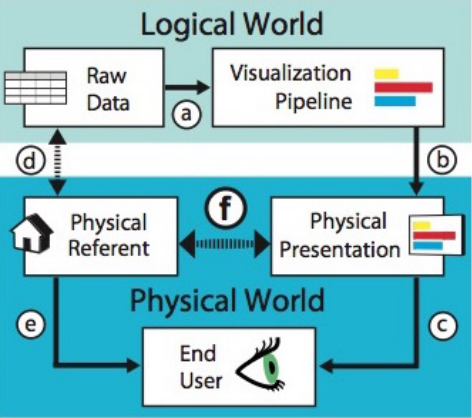
\includegraphics[width=0.5\textwidth]{resources/fundamentals/situated_visualization/spacially_situated_visualization_model.png}
	\caption{Konzeptionelles Model zu Situated Visualization Quelle: \cite[S.~192]{ElSayedNevenA.M.BruceH.ThomasRossT.Smith2015}}
	\label{img:situated_visualization_concept}
\end{figure}

% spacially situated visualization
Dieses Modell (siehe Abbildung \ref{img:situated_visualization_concept}) erweitert die konventionelle Visualisierung der logischen Welt (Abbildung \ref{img:situated_visualization_concept} oberer Abschnitt) um die der physischen Welt (Abbildung \ref{img:situated_visualization_concept} unterer Abschnitt). 
Die durchgängig dargestellten Pfeile (Abbildung \ref{img:situated_visualization_concept} (a), (b), (c) und (e)) zeigen den Informationsfluss zwischen den einzelnen Komponenten, die gestichelten Pfeile (Abbildung \ref{img:situated_visualization_concept} (d) und (f)) die konzeptionellen Beziehungen. Der Informationsfluss beginnt bei den Rohdaten in der oberen linken Ecke der Darstellung. Die Rohdaten durchlaufen den Visualisierungs-Pipeline und werden in ein vom Menschen besser interpretierbare visuelle Form umgewandelt (Abbildung \ref{img:situated_visualization_concept} (a -> b)). Die Verbindung zwischen logischer und physischer Welt wird mithilfe zweier Beziehungen hergestellt (b und d). 
Die physische Präsentation der Daten (Abbildung \ref{img:situated_visualization_concept} (b)) stellt die Präsentation der Daten in visueller Form in der Realen Welt dar. 
Dies könnte zum Beispiel eine Visualisierung in Form einer Annotation sein, welches der Betrachter durch eine Datenbrille auf einem physischen Gegenstand sieht, eine Auflistung von Daten welches 
auf dem  Display eines Smartphones oder Tablett angezeigt wird oder ein Preisschild welches in ausgedruckter Form an ein physisches Gegenstand angebracht wurde.

Die zweite Beziehung besteht zwischen Rohdaten und physischen Referenten . Diese Beziehung ist konzeptionell, da Datensätze sich auf mehrere unterschiedliche Referenten beziehen können. 
Der Grad, in wieweit der physische Referent und die physische Präsentation gleichzeitig wahrgenommen werden können hängt von der räumlichen Distanz zwischen diesen beiden ab. 

Der Betrachter könnte die Daten mithilfe von Augmented Reality, auf dem physischen Referenten betrachten. Der Betrachter könnte vor dem physischen Referenten stehen und die Daten zu dem Referenten auf
dem Bildschirm seines Smartphones betrachten. Der Betrachter könnte aber auch räumlich entfernt vom physischen Referenten sein, sodass er diesen nicht sehen kann und die Daten auf einem Ausgabegerät 
wie einem Computerbildschirm betrachten. 

%Physically- vs. Perceptually-Situated Visualizations 
\cite[S.~194]{ElSayedNevenA.M.BruceH.ThomasRossT.Smith2015} Da Distanzen jedoch relativ zu Größe von Objekten wahrgenommen werden, kann die physische und die wahrgenommene Distanz zwischen dem Physischen Referenten und der Physischen Präsentation stark voneinander abweichen. Wenn beide Objekte zum Beispiel nur wenige cm groß sind, kann ein Abstand von einem Meter sehr groß erscheinen, während der gleich Abstand für ein sehr großes Objekt, wie zum Beispiel ein Berg in einer Landschaftsansicht, zum Beispiel sehr klein erscheint. 

%Zeitlich distanz (temporal)
\cite{WesleyWillettYvonneJansen} Neben der räumlichen Distanz muss auch die zeitliche Distanz zwischen dem aktuellen Zustand des Physischen Referenten und die der physischen Präsentation hinsichtlich dessen 
Aktualität betrachtet werden. 
Die zeitliche Distanz ist die zeitliche Abweichung zwischen den Daten die dem aktuellen Zustand des physischen Referenten entspricht, und den Daten welche in der Physischen Präsentation visualisiert werden.
Werden beispielsweise Temperaturwerte die ein Temperatursensor an einem physischen Objekt anzeigt betrachtet und es wird der aktuell gemessene Wert angezeigt gibt es keine zeitliche Distanz. Wird jedoch ein
historischer Wert angezeigt oder eine Vorhersage, kann die zeitliche Distanz stark variieren.

%embedded visualisierung
\begin{figure}[H]
	\centering
	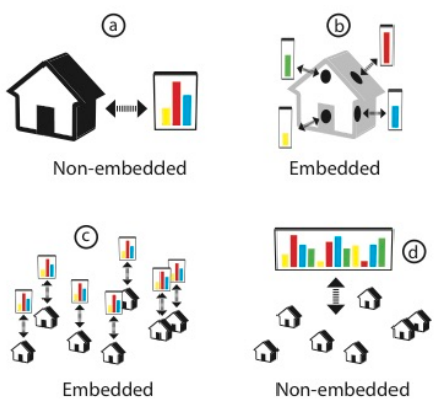
\includegraphics[width=0.5\textwidth]{resources/fundamentals/situated_visualization/embedded_visualization.png}
	\caption{Embedded und Nicht-Embedded Situated Visualisierungen}
	\label{img:embedded_visualization}
\end{figure}

\cite[S.~195]{ElSayedNevenA.M.BruceH.ThomasRossT.Smith2015} Embedded Visualization stellen eine besondere Art von Situated Visualization dar, welche sehr stark in die physische Umgebung integriert sind. 

Abbildung \ref{img:embedded_visualization} zeigt eingebettete und nicht eingebettete (Situated) Visualisierungen. [Kim Marriott et. al Seite 202] Ist ein Objekt aus mehreren Einzelteilen 
zusammengesetzt und die Daten zu den Einzelteilen, werden in einer Visualisierung in der Nähe des Objektes dargestellt, gilt die Visualisierung als Situated, jedoch nicht als Embedded (Abbildung \ref{img:embedded_visualization} (a)).
Werden die Daten zu den Einzelteilen, jeweils in der Nähe der jeweiligen Einzelteilen dargestellt, gilt die Visualisierung als Embedded (Abbildung \ref{img:embedded_visualization} (b)). Ist ein, Einzelteil jedoch nur einmal in einem Produkt vorhanden (zum Beispiel ein Motor in einem Auto), gilt die Visualisierung zu diesem Einzelteil nicht als Embedded. 

Embedded Visualization geht davon aus, dass mehrere Teil-Visualisierungen zu den jeweiligen physischen Referenten entsprechen. Befinden sich in einem Haus beispielsweise mehrere Steckdosen und der Stromverbrauch 
für jede Steckdose wird jeweils in der Nähe der jeweiligen Steckdose visualisiert, gilt die Visualisierung als Embedded. Gibt es in dem Haus jedoch nur eine Steckdose, gilt die Visualisierung nicht mehr als
Embedded.

\vspace{15mm} 
\begin{figure}[H]
	\centering
	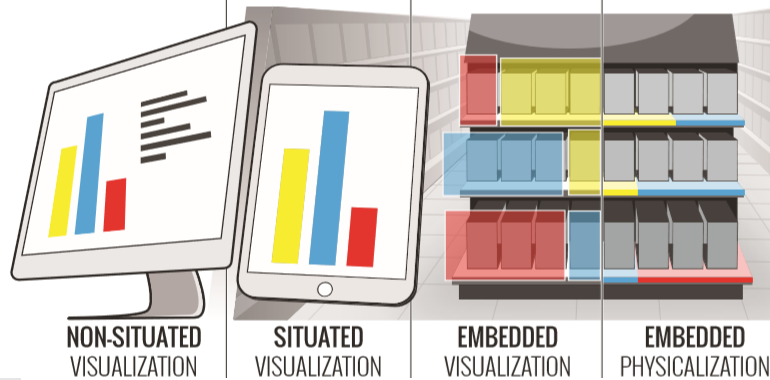
\includegraphics[width=0.5\textwidth]{resources/fundamentals/situated_visualization/Illustration_situated_embedded_visualization.png}
	\caption{Illustration mit unterschiedlichen Visualisierungen am Beispiel von Produkten in einem Supermarkt-Regal}
	\label{img:Illustration_situated_embedded_visualization}
\end{figure}

Mit Hilfe der Illustration in Abbildung \ref{img:Illustration_situated_embedded_visualization} zeigen \cite{WesleyWillettYvonneJansen} am Beispiel von Produkten, 
welche in einem Supermarkt in einem Regalen platziert sind, die Eigenschaften unterschiedlicher Visualisierungen und die damit verbundenen Vor- und Nachteile der jeweiligen Visualisierungsform. 

Der Vorteil von Non-Situated Visualisierungen (Abbildung \ref{img:Illustration_situated_embedded_visualization} ganz links) ist, dass diese flexibler hinsichtlich Standort 
der Nutzung und Hardwareanforderungen gestaltet werden können. Der Betrachter kann sich in dieser Form der Visualisierung räumlich getrennt von den Produkten befinden und die Visualisierung 
auf einem beliebigen Display wie zum Beispiel einem Computerbildschirm, auf dem Display eines Smartphones oder Tablett ansehen. Der Nachteil dieser Art der Visualisierung ist jedoch dass kein 
direkter Bezug zwischen den angezeigten Informationen und den physischen Produkten bzw. Produktteilen hergestellt werden kann. 

Am Beispiel von (Abbildung \ref{img:Illustration_situated_embedded_visualization} ganz links), wäre dem Betrachter, ohne die Unterstützung einer Beschreibung der Lage wo sich die Produkte im 
Supermarkt befinden oder mit Hilfe einer Karte, nicht möglich, eine Beziehung zwischen der, physischen Platzierung der Produkte im Verkaufsraum und deren Umsatz herzustellen.

Situated Visualization ermöglicht dem Betrachter, Produkte bzw. Produktteile und Visualisierungen zu diesen, zur gleichen Zeit betrachten zu können. Dies bring den Vorteil dass eine Beziehung 
zwischen Lage und Ausrichtung der Produkte bzw. Produktteile und den visualisierten Informationen hergestellt werden kann. Diese Form der Visualisierung erfordert jedoch, dass sich 
der Betrachter räumlich nahe am Produkt befindet und die Visualisierung auf einem mobilen Endgerät anzeigt wird.

Embedded Visualization ermöglichen dem Betrachter, die Visualisierung der Daten unmittelbar an den jeweiligen Produkten bzw. Produktteilen zu betrachten ohne den Blick von diesen abwenden zu müssen. 
Dies bringt den Vorteil dass der Betrachter während er die Visualisierung betrachtet, seinen Blick nicht vom Produkt bzw. Produktteil abwenden muss und Informationen zur direkten Umgebung des Produktes bzw. Produktteiles wahrnehmen kann. Diese Form der Visualisierung erfordert dass sich der Betrachter vor den entsprechenden Produktteilen befindet und Ausgabetechniken verwendet werden, welche die Informationen unmittelbar an den 
Produktteilen anzeigen (z. Bsp. AR).

Am Beispiel von (Abbildung \ref{img:Illustration_situated_embedded_visualization} zweite von rechts) ist dem möglich Betrachter Informationen zur unmittelbaren Umgebung der Produkte (zum Beispiel eine zu schwache Beleuchtung, einen unangenehm riechenden Geruch, ein Windzug, usw.) wahrzunehmen, während er die Visualisierung (welches ihm zum Beispiel zeigen könnte dass der Umsatz für diese Produkte während der vergangenen Monate zurück gegangen ist) zu diesen Produkten unmittelbar an den Produkten betrachtet.  

%Facsimiles
\cite{WesleyWillettYvonneJansen}Eine Möglichkeit, um Daten im Kontext zu physischen Objekten zu visualisieren, ist auch über die Verwendung von so genannten Faksimiles möglich. Diese sind detailgetreue, skalierbare Nachbildungen von Objekten, oder eine Instanz eines Objektes, welche durch eine Klasse oder ein Modell klar definiert ist. Ein Faksimile wird für gewöhnlich verwendet, falls die Visualisierung am echten physischen Referenten schwierig bis unmöglich ist: Dies ist der Fall, wenn zum Beispiel sehr klein (z.Bsp. Atome), sehr groß (z Bsp. ein Flussverlauf) zu weit entfernt (z. Bsp: auf einem anderen Planeten) oder sehr fragil bzw. wertvoll sind (z. Bsp. ein Gemälde). 
In solchen Begebenheiten kann die Nutzung von Faksimiles die räumliche Distanz zum betrachtenden Objekt reduzieren und es damit zugänglicher machen. Ein Faksimile kann wenn diese mit ausreichender detailgetreue nachgebildet ist wie der eigentlichen physische Referent betrachtet werden. Die Nutzung von Faksimiles verringert jedoch, die Möglichkeit für den Betrachter, den eigentlichen Referenten zu verändern oder wichtige Details zu betrachten. Dies kann durch den Einsatz von Telepräsenz\footnote{Telepräsenz ist eine Form von Videokonferenz und beschreibt die Möglichkeit, virtuell an entfernten Orten Präsent zu sein. Siehe: https://www.itwissen.info/Telepraesenz-telepresence.html [Zuletzt aufgerufen am: 28.06.2018]} werden. 

\subsection{(Situated Visualization) - Techniken und Herausforderungen}

Situated Visualization 
%Herrausforderungen: Unordnung duruch zu viele Daten (Überlagerung). Generell auch bei anderen visualisierungen. Durch limitierter Platz bei AR manchmal besonders verschlimmert. %Registrierungsfehler führen zur falschen platzierung von visualisierungen. 

% Störende\ Ungünstige Visualisierung. Auch wenn Registrierung theoretisch ganz fehlerfrei funtionieren würde, ungünstig sein und die Fähigkeit des Nutzers wichtige Informationen von nicht relevanten Informationen. 

% In folgendem werden Techniken für die Bewältigung dieser Herrausforderungen vorgestellt. 

Data Overlay 

% la

% Labeling und Annotationen

\section{Computerunterstützte Kollaboration}

Durch die Verwendung des zu entwickelnden Systems, sollen Anwendungsszenarien unterstützt werden, in welchen Nutzer, 
über Feedbacks auf Produkten bzw. Produktteilen kommunizieren können. Diese Kommunikation soll eine Kollaboration von 
mehreren Nutzern, mit dem Produkt im Mittelpunkt zu ermöglichen und zum Ziel haben, die Qualität der Produkte und die 
damit verbundene Kundenzufriedenheit zu verbessern.     

In der computerunterstützten, kooperativen Zusammenarbeit (en. Computer-Supported Cooperative Work (CSCW)) 
ist eine Kategorisierung die Rodden in \cite[S.~2]{Rodden1992} beschreibt, sehr verbreitet.  


Rodden betrachtet bei dieser Kategorisierung zwischen Nutzern zwei Dimensionen der Kommunikation zwischen Nutzern: 
Die räumliche Distanz zwischen Nutzern sowie die zeitliche Differenz im Nachrichtenaustausch, dabei erfolgt einen Unterteilung zwischen 
Remote oder Co-Located und Synchron oder Asynchrone Kommunikation.

Die zeitliche Dimension definiert, ob mehrere Nutzer zur gleichen Zeit (synchron) miteinander kommunizieren 
oder zu unterschiedlichen, also (asynchron/ zeitlich unabhängig voneinander) kommunizieren. Die räumliche Dimension 
gibt Aussage darüber, ob sich die Nutzer während der Kommunikation am gleichen Ort befinden (Co-located) oder räumlich getrennt voneinander sind (Remote). 

\cite[S.~188]{ElSayedNevenA.M.BruceH.ThomasRossT.Smith2015} beschreiben darüber hinaus eine Mischform von Remote und Co-located Kommunikation. 
Bei dieser Form von Kollaboration können eine Teilmenge der Nutzer sich am gleichen Ort befinden, während ein anderer Teil entfernt, 
also (Remote), mittels Telepräsenz an der Kommunikation teilnehmen. 

Schmalstieg und Höllerer \cite{DieterSchmalstieg2016} beschreiben auf Grundlage dieser Unterteilung mögliche 
Anwendungsgebiete für AR Systeme (Siehe Tabelle \ref{tab:categorycscw}).

\cite{DieterSchmalstieg2016} In Co-Located und synchronen Anwendungsszenarien (z. Bsp. eine Besprechung in einem Besprechungsraum), können 
Augmented Reality Anwendungen, die Nutzern dabei unterstützen, Informationen im gemeinsamen Raum zu betrachten zu manipulieren und zu diskutieren. 

In Remote und synchronen Szenarien können AR-Systeme es ermöglichen dass ein Nutzer (Nutzer 1), einem anderen Nutzer (Nutzer 2 welcher räumlich getrennt von Nutzer 1 befindet), 
Informationen über dessen reale Umgebung zu zeigen kann (z. Bsp. Installations- oder Reparatur-Anleitungen). \footnote{Ein AR App der Firma PTC welches Nutzern über eine synchronen Kommunikation, Informationen in die Umgebung des jeweils anderen einzublenden: https://www.ptc.com/de/news/2017/vuforia-chalk [Zuletzt aufgerufen am 21.08.2019]} 

\begin{table}[htbp]
\caption{Kategorisierung Computer unterstützter Kooperationssysteme mit Bezug zu AR. \\Quelle: \cite[S.~362]{DieterSchmalstieg2016}}
	\begin{center}
		\begin{tabular}{|l|ll|}
		\hline
		 & \textbf{Co-located} & \textbf{Remote}\\
		\hline
		\textbf{Synchronous} &  AR shared space & AR telepresence \\
		\textbf{Asynchronus} & AR annotating/ browsing (in-situ) & Generic sharing\\
		\hline
		\end{tabular}
	\end{center}
	\label{tab:categorycscw}
\end{table}

\cite[S.~362]{DieterSchmalstieg2016} Zu den Anwendungsszenarien für asynchrone Kommunikation in AR Anwendungen zählt das Erstellen von Annotationen in der 
physischen Umgebung und das spätere, an Ort und Stelle, Durchforsten und Bearbeiten dieser Annotationen durch andere Nutzer.		

\begin{comment}
Rodden beschreibt in \cite{Rodden1992} 

- Erzeugung von viel breitere Gruppendiskussionen und Aufzeichnung dieser Diskussionen(Report) (z.Bsp. Foren, Community Beiträge).\cite{Rodden1992} cite{Benbunan-Fichet} 
- Gibt Nutzern die Flexibilität, immer dann Beiträge zu erstellen wenn diese Zeit dazu haben.
- Ermöglicht, Nutzern sich mit Teilproblemen befassen für das sie sich am besten befähigt fühlen.
- Zusammensetzung von Informationen aus eine Vielzahl von Quellen und Nutzern


Roden \cite{Rodden1992} ordnet asynchrone Kollaboration zu den Co-Authoring Systemen. Diese sind Systeme, welche mehreren Nutzern, asynchrone Zusammenarbeit 
an einem Artefakt ermöglichen. Jeder Nutzer kann dabei an einem Teil des Dokumentes arbeiten und die Ergebnisse werden zusammengeführt. Asynchrone Kollaboration 
unterstützt laut Rodden einen Grundlegenden Teil von Kooperation, indem es die 
 can produce broader discussions and more complete reports from group discussions than their face-to-face counterparts
 enabling people to contribute whenever they have time to provide input
 they can work on the part of the problem that they feel most qualified to address
 can combine information from a variety of sources

 Co-authoring systems aim to support some of the most fundamental parts of cooperation by supporting the negotiation processes
 for commenting - multiple users working on 
 store and forward and real-time communication systems

notwendigkeit für unterscheidung zwischen private, public oder direkte nachrichten 

[Rodden seite 20]
 [Rodden seite 24] Co-authoring systems aim to support some of the most fundamental parts of cooperation by supporting the negotiation processes % for commenting %multiple users working on % [Rodden seite 24]store and forward and real-time communication systems. %
The general model adopted by these systems is that of asynchronous co-operation with each user working independently on a portion of the document. Reviews and comments are added to the document by annotating sections of the document. 

\end{comment}

\section{Usability}

Nach der Implementierung eines digitalen Prototypen, soll im Rahmen einer Nutzerstudie die Usability (dt. Benutzbarkeit) des Prototypen evaluiert werden.
Daher wird in diesem Abschnitt, die Definition von Usability näher betrachtet. Anschließend wird ein Einblick in Usability Engineering gegeben welches eine etablierte Herangehensweise für
die Gestaltung und Entwicklung von Systemen mit hohen Usability Anforderungen ist. 

\subsection{(Usability) - Definition} \label{UsaDef}

% Begiffserklärung von Usability
In der Normreihe ISO 9241 welches als ein internationaler Standard, Richtlinien für die Gestaltung von Mensch-Computer-Interaktionen beschreibt, wird im ISO Norm 9241-11,  Usability (zu dt. Benutzbarkeit) wie folgt definiert:

``\textit{Das Ausmaß, in dem ein Produkt durch bestimmte Benutzer in einem bestimmten Nutzungskontext genutzt werden kann um bestimmte Ziele effektiv, effizient und zufriedenstellend zu erreichen.}``

%Die Benutzbarkeit eines Systems muss im Kontext seiner Verwendung beurteilt werden.[Michael Richter, Markus Flückiger]
Dass die Usability eines Systems nach dessen Nutzungskontext zu bewerten ist verdeutlichen \cite{MichaelRichter2016} an einem konkreten Beispiel für die Erfassung 
von Kurznachrichten (SMS) mit dem Aufkommen von Mobiltelefonen. Bevor Smartphones mit Touch-Displays verbreitet waren, hatten Mobiltelefone oft rein numerische Tastaturen sodass, das Erfassen 
von Textnachrichten über die Nutzung der numerischen Tasten erfolgen musste. Indem zum Beispiel in kurzen Zeitabständen zwei mal auf die Taste ``2`` gedrückt wurde, wurde zu Beispiel der Buchstabe 
``B`` eingegeben. Diese Eingabemethode wurde oftmals von vielen Nutzern als umständlich empfunden. Jedoch konnte auf diese Weise effizient und zufriedenstellend die Aufgabe, eine Kurznachricht 
zu erfassen erfüllt werden. Zudem war diese Methode einfach zu erlernen und einprägsam. Somit wies dieser Ansatz für den damaligen Stand der Technik eine hohe Usability auf. 

% Eine Teilmenge der Systemazeptanz 
Nielsen stellt \cite{Nielsen1994} Akzeptanzkriterien für ein Systeme vor und stellt Usability als eine Teilmenge die dieser Kriterien vor.
Akzeptanzkriterien unterteilt er in soziale und praktische Kriterien.

Soziale bzw. ethische Akzeptanzkriterien sind solche, welche die Nutzer von der Nutzung eines Systems abhalten, auch wenn praktische Akzeptanzkriterien sehr gut erfüllt werden. 

Um die gewünschte Funktionalität zu ermöglichen, werden mit Augmented Reality Anwendungen viele Informationen über die Umgebung des Nutzers erhoben.\cite[S.~3]{Roesner2013} Es wird auf die Kamera, gegebenenfalls auf den Lautsprecher sowie verschiedene Sensoren wie z. Bsp. den Gyroskop, Accelerometer usw. zugegriffen. Dies birgt Risiken dass diese Daten missbräuchlich genutzt, gestohlen und die Privatspähehe von Nutzern verletzt werden können. \cite[S.~9]{Templeman2012} Die Studie PlaceRaider beweist, dass mithilfe von Kamera und Sensordaten eines Smartphones die Umgebung des Nutzers detailliert genug rekonstruiert werden kann, um sensible Informationen wie z. Bsp. Kontodaten auf einem Kontoauszug ablesen zu können. \cite{Roesner2013,Lebeck2018} stellen weitere Risiken für die Beeinträchtigung der Privatsphäre von Nutzern vor welche als soziale Akzeptanzkriterien bei der Gestaltung von Augmented Reality Systemen beachtetet werden sollten. 

Unter den praktischen Kriterien sowie Usability (zu dt. Benutzbarkeit) auf. Die Eigenschaft Benutzbarkeit gliedert er in die Eigenschaften Nützlichkeit (en. Utility) und Gebrauchstauglichkeit (en. Usability) auf. Unter Utility (zu dt. Nützlichkeit) ist zu verstehen ob ein System mit den Funktionalitäten die es bereitstellt in der Lage ist, die Aufgabe zu erfüllen wozu sie konzipiert wurde.

Die Eigenschaft Benutzbarkeit gliedert Nielsen in folgende fünf Teileigenschaften: 

\begin{itemize}
	\item Einfach zu erlernen.
	\item Effizient in der Nutzung.
	\item Leicht zu merken. (Ein Nutzer welcher das System bereits einmal verwendet hat, sollte in der Lage sein nach einer längeren Pause das System nutzen zu können ohne es erneut erlernen zu müssen.)
	\item Wenig Fehler. (Das System sollte während der Nutzung zu möglichst wenig Fehler führen. Im Falle das Fehler auftreten, sollte es möglich sein dass sich das Systems von diesen Fehlern erholt sodass die Nutzung des Systems fortgeführt werden kann.)
	\item Subjektive Zufriedenstellung (Das System sollte angenehm zu nutzen sein. So dass Nutzer auch subjektiv zufriedengestellt werden während sie das System nutzen.)
\end{itemize}

%7 Kritärien nach ISO 9241 Teil 110 - ASSEFIL) 
Im ISO Norm  9241-110 sind diese Kriterien, als Grundsätze zur Dialoggestaltung wie folgt aufgeführt:

\begin{itemize}
	\item Aufgabenangemessenheit \footnote{Beispiele für Aufgabenangemessenheit ab Seite 5: https://www.medien.ifi.lmu.de/lehre/ss16/id/ISO\_9241-10.pdf [zuletzt aufgerufen am: 26.06.2019]}
	\item Selbstbeschreibungsfähigkeit
	\item Steuerbarkeit
	\item Erwartungskonformität
	\item Fehlertoleranz
	\item Individualisierbarkeit
	\item Lernförderlichkeit
\end{itemize}

\subsection{Usablity Engineering}

\cite{MichaelRichter2016} Im laufe der Zeit haben sich verschiedene Fachrichtungen (wie z. Bsp: Human Computer Interaction (HCI), Human Factors, Interaction Design, Usability Engineering, 
User centered Design (UCD), User Experience (UX) und Design Thinking) entwickelt welche nutzenorientierte Methoden für die Entwicklung von Technologien und neuen Anwendungen verfolgen. 

% Usablity Engineering
\cite[S.~14]{MaryBethRossonJohnM.CarrollDianeD.Cerra2002} Als eines dieser Fachrichtungen wurde die Fachrichtung Usablity Engineering von Usability Fachleuten bei Equipment Corporation ins Leben gerufen.  
Der Begriff Usability Engineering steht für die Konzeption, die Techniken für die Planung, Verifizierung und Abdeckung von Usability Zielen eines Systems. Das Ziel von Usability Engineering ist, 
messbare Usability Ziele in den frühen Phasen des Softwareentwicklungsprozesses zu definieren und einen Rahmen zu schaffen diese Ziele im laufe der Entwicklung stetig überprüfen zu können 
um sicherstellen zu können dass diese erreicht werden.

Nielsen beschreibt in \cite{Nielsen1994} Phasen den Entwurf und Entwicklung von Software Projekte mit der Anwendung von Usability Engineering Methoden durchlaufen. 
Im folgenden werden einige dieser Phasen zusammenfassend erläutert: 

\vspace{5mm}
\textbf{Benutzerprofile}\label{userprofile}  
 
\cite[S.~73]{Nielsen1994} In dieser Phase der Usability Engineering werden alle Nutzer identifiziert, die mit dem zukünftigem System in Berührung kommen werden. Als Nutzer werden Personen verstanden welche mit dem System oder mit Artefakten die durch Systems entstehen in Berührung kommen werden. Dies kann Personen beinhalten welche das System installieren, konfigurieren, warten, administrieren sowie Endnutzer
des Systems oder aber auch Personen die das System selbst nicht nutzen jedoch Ergebnisse die durch das System entstehen erhalten werden. In einigen Fällen, ist es einfacher potenzielle Nutzer eines neuen  Systems zu identifizieren und deren Charakteristiken zu analysieren. Dies ist der Fall wenn Produkte für eine ganz bestimme Nutzergruppe vorgesehen sind. 
Zum Beispiel für Produkte welche in einer bestimmten Abteilung eines Unternehmens in Einsatz kommen sollen. Schwieriger ist die Analyse von Nutzern hingegen für Produkte welche von einer breiteren Menge von Nutzern genutzt werden sollen. 

Folgende Informationen sollten über die Nutzer erhoben und analysiert werden: Der Erfahrungsstand des Nutzers (z Bsp. in Verwendung von solchen Systemen und Endgeräten), Bildungsstand, Alter des Nutzers, Arbeitsumgebung, Lebensumstände, usw. Dieser Schritt ist wichtig um die Lernfähigkeit von Nutzern besser einschätzen zu können und so Kriterien für die Komplexität der Nutzeroberfläche zu bestimmen.

% task analysis 
\textbf{Aufgabenanalyse}\label{task_anlyse}  

\cite[S.~75]{Nielsen1994} Sobald die Nutzer identifiziert und deren Eigenschaften sowie Bedürfnisse analysiert wurden, werden die Ziele und Aufgaben der Nutzer analysiert. Wie bewältigen die Nutzer aktuell Aufgaben um ihre Ziele zu erreichen? Hierbei sollte beobachtet werden welche Informationen die Nutzer benötigen, welche Ausnahme oder Not Situationen auftreten und wie die Nutzer in diesen Situationen handeln. 
Es sollte beobachtet werden ob die Nutzer das aktuell verwendete System in irgendeiner weise umgehen (engl. Workarounds anwenden). Zudem sollten die im Bezug auf die zu lösende Aufgabe, verwendeten 
Terminologien festgehalten werden. Diese können später als eine Quelle für Metapher bei der Gestaltung der neun Nutzeroberfläche verwendet werden. 

% functional analysis TODO: Füge Referenz mit seitenzahl hinzu
\cite[S.~77]{Nielsen1994} Im nächsten Schritt werden die benötigten Funktionalitäten des neuen Systems analysiert und Möglichkeiten erforscht wie diese mit dem neuen System erzielt werden können. 
Es ist wichtig dass in diesem Schritt die Mögliche Umsetzung der Funktionalitäten sich nicht ausschließlich an Lösungen von bereits bestehenden Systemen orientiert sondern 
bessere geeignete Umsetzungsmöglichkeiten erkundet werden.

% evolution of the user TODO: Füge Referenz mit seitenzahl hinzu
\cite[S.~78]{Nielsen1994} Zuletzt werden in dieser Phase Möglichkeiten erforscht wie sich das Nutzungsverhalten der Nutzer über die Zeit, mit der Nutzung des neuen Systems entwickeln könnte. Dieser Schritt wird  
benötigt um das neue System flexibel genug und offen für neue Anforderungen gestalten zu können. 

\vspace{5mm} 
\textbf{Analyse bestehender Produkte} 
 
\cite[S.~78]{Nielsen1994} In dieser Phase werden bestehende Produkte mit ähnlichem Aufgabenfeld analysiert. Diese können für die Konzeption des neuen Systems als Prototypen dienen. 
Da bestehende Systeme vollständig umgesetzte Funktionalitäten beinhalten, können diese einfach getestet werden.    
Diese Systeme können heuristisch evaluiert werden, es können Nutzer Studien durchgeführt werden oder es kann eine vergleichende Analyse durchgeführt werden falls mehrere Systeme zur 
Verfügung stehen. Auf Basis der Informationen die, in der Phase ``Benutzerprofile`` zusammengetragen wurden, wird in dieser Phase analysiert wie gut die Funktionalitäten und Interaktionstechniken 
bestehender Systeme die Nutzer bei der Umsetzung ihrer Aufgaben unterstützen. Zusätzlich können technischen Produktrezessionen in dieser Phase auch hilfreiche Informationen über bestehende Systeme geben. 
Da nicht alle Aufgaben bereits eine Software Lösung existiert, schließt Nielsen in dieser Phase die Betrachtung von Lösungen welche nicht aus dem Software bzw. Computer Bereich stammen ein. 

\vspace{5mm} 
\textbf{Usability-Ziele festlegen} 

Wie im Abschnitt \ref{UsaDef} beschrieben, setzt sich die Usability eines Systems nicht nur aus einer Eigenschaft zusammen sondern gliedert sich in mehrerer Teileigenschaften wie Erlernbarkeit, Fehlertoleranz usw. \cite[S.~79]{Nielsen1994} Oft ist es nicht möglich alle Usability Kriterien mit gleicher Gewichtung zu priorisieren. In dieser Phase werden auf Grundlage der erstellten Benutzerprofile sowie der Aufgabenanalyse, Prioritäten für die einzelnen Usability Eigenschaften definiert. 

Dafür werden die Usability Eigenschafen operationalisiert und in messbaren Zielen ausgedrückt. Meistens werden Messintervalle für angestrebte Werte, für minimal zu erreichende Werte und theoretisch optimale Werte definiert. Als minimal zu erreichende Werte sind, gelten der Regel Werte welche aktuell mit dem System erreicht werden kann. Usability Ziele für neue Versionen von bestehenden Systemen oder für Systeme für welche vergleichbare andere Systeme existieren, festzulegen ist deutlich einfacher als für neue Systeme wozu keine Vergleichswerte vorliegen. Ein Vorgehen für solche Systeme ist, einige mit dem System zu lösende Aufgaben zu definieren und mehrere Usability Spezialisten nach realistischen Werten zu fragen welche erzielt werden könnten.

\vspace{5mm} 
\textbf{Prototypen und Szenarien}

\cite[S.~93]{Nielsen1994} Die Implementierung eines Systems sollte nicht auf Basis der Gestaltung von Benutzeroberflächen in den frühen Phasen der Konzeption stattfinden. 
Stattdessen können Prototypen in den frühen Phasen eingesetzt werden. Auf diese weise können, Zeit und kostensparend Prototypen des finalen Systems in den frühen Gestaltungsphasen
evaluiert werden. Prototypen lassen sich in zwei Dimensionen unterteilen (Abbildung \ref{img:ver_hor_protptypes}): 

\begin{figure}[H]
	\centering
	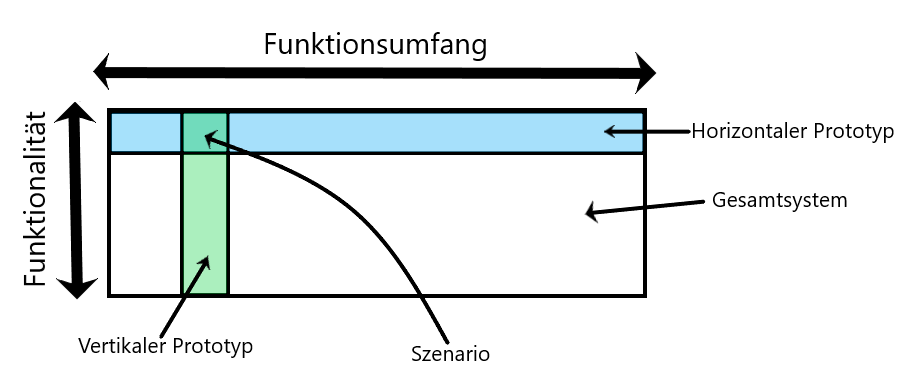
\includegraphics[width=0.8\textwidth]{resources/fundamentals/hor_ver_prototypes.png}
	\caption{Schematische Darstellung von horizontalen und vertikalen Prototypen. Quelle: In Anlehnung an \cite[S.~94]{Nielsen1994}}
	\label{img:ver_hor_protptypes}
\end{figure}

In die horizontale Dimension haben Prototypen einen breiteren Funktionsumfang beinhalten jedoch wenig bis keine Funktionalität. Horizontale Prototypen eignen sich sehr gut um ein Überblick über den Funktionsumfang des Systems zu gewinnen. Jedoch wirken Test Szenarien mit diesen Prototypen eher unrealistisch da durch die fehlende Funktionalität keine Aufgaben mit den Funktionen die der Prototyp 
bereitstellt gelöst werden können.\\
Sind Prototypen in die vertikale Richtung gestaltet, sind sie in der Funktionsumfang eingeschränkt bieten jedoch mehr Funktionalität. Diese Prototypen eignen sich sehr gut um 
besondere Aspekte eines Systems in aller Tiefe zu beleuchten. Dadurch eignen sich diese Prototypen sehr gut um bestimmte Funktionen möglichst in die Tiefe, unter realistischen 
Umständen zu testen und richtigen Aufgaben zu lösen.

Szenarien beschreibt Nielsen in \cite[S.~99]{Nielsen1994} als minimalistische Prototypen welche die Einschränkungen von horizontaler und vertikaler Prototypen vereinen. 
Nutzer können nicht mit Daten interagieren (Einschränkung horizontale Prototypen) und Nutzer können sich nicht frei im System bewegen (Einschränkung vertikaler Prototypen).
 \cite[S.~100]{Nielsen1994}Weiter definiert Nielsen, Szenarien wie folgt. 
 
 Ein Szenario beschreibt:

\begin{itemize}
	\item Einen individuellen Nutzer
	\item welcher unter bestimmten Umständen
	\item über ein bestimmtes Zeitintervall (Im Kontrast zu anderen Prototypen beinhalten Szenarien zusätzlich eine explizite Zeitdimension in welcher bestimmt wird welche Reaktion auf eine bestimmte Aktion folgt.)
	\item eine spezifischen Teil eines Computersystems nutzt
	\item um ein bestimmtes Ergebnis zu erzielen
\end{itemize}

 \cite[S.~101]{Nielsen1994} Aus Szenarien können, wenn diese ausreichend detailliert gestaltet Nutzertests verwendet werden. Beispielsweise können auf Basis von Szenarien Papierprototypen erstellt werden 
 und diese von Nutzern getestet werden um Aufgaben zu lösen. 

\subsection{Personas}

% Personas




 \clearpage
\chapter{Analyse} \label{anlayse_capter}

In diesem Kapitel wird der Stand der Forschung zu Themen welche für diese Arbeit eine hohe Relevanz darstellen behandelt. Dazu zählen wie Annotationen in virtuellen Umgebungen, das Zeigen und Auswählen in AR sowie die Kundeniteration mit immersiven Methoden.

\begin{comment}
\section{Augmented Reality Frameworks}

In diesem Abschnitt wird eine Übersicht über Augmented Reality Framework nach aktuellem Stand der Technik gegeben.

%ARKit ARCore SLAM!
Zum aktuellen Stand der Technik 

%Vuforia, Wikitude... Marker, Natural Feature, 3dObject

%Visionlib 3D Objekt spezialisiert. 

%Unterschide 3D Objekt basiert Vuforia und visionlib: Vuforia - keine Objekte mit geringer geometrischen eigenschaften. Vuforia, bewegungsempfindlich. 

%Vuforia kann mit ARCore oder ARKit kombiniert werden!
\end{comment}

\section{Informationsdarstellung in virtuellen Umgebungen}\label{brand_abschnitt}

Mit Anwendung des digitalen Prototypen sollen Feedback in Form von Annotationen auf dem physischen Produkt dargestellt werden. 
In diesem Abschnitt werden Forschungen zu Annotationen in Virtuellen Umgebungen insbesondere der Usability-Aspekte dieser Darstellungsform näher betrachtet. 

\citeauthor{Brandenburg2019} befasst sich in ihrer Arbeit mit unterschiedlichen Informationsdarstellungsformen in virtuellen Umgebungen.
Sie vergleicht hierbei in einer Studie zwei unterschiedliche Darstellungsformen in einer CAVE \footnote{CAVE kurz für \textit{Cave Automatic Virtual Environment}, bezeichnet einen Raum in welcher drei bis 6 Wände Projektionsflächen sind und dem Nutzer durch das Tragen von Schutterbrillen ein Eindruck von ... erscheint } hinsichtlich Usability-Aspekte für virtuelle Design-Review Prozesse in der virtuellen Produktentstehung. Dabei wird ein besonderer Fokus auf die Art der Aufgabe der Review-Teilnehmer gelegt.
\cite[S.~48]{Brandenburg2019}

Bei einer virtuellen Design-Review wird das 3D-Modelle eines Produktes bzw. verschiedene Ausführungen davon von einem interdisziplinären Reviewteam betrachtet um Entscheidungen zu treffen. 
Herbei werden neben dem 3D-Modell des Produktes Informationen zum Produkt bzw. zu den einzelnen Produktteilen betrachtet welche für die Entscheidungsfindung relevant sind. \cite[S.~32]{Brandenburg2019}
 
In Anlehnung an \cite{Polys2004} \cite{Polys2007} identifiziert \citeauthor{Brandenburg2019} zwei unterschiedliche Aufgabentypen welche einen Einfluss auf die jeweiligen Darstellungsformen haben: Such und Vergleichsaufgaben. 
Eine Suchaufgabe kann dabei z. B. folgende Frage sein: ``Wo ist der Motor?`` eine Vergleichsaufgabe hingegen: ``Was befindet sich im Kofferraum und wie wird es bezeichnet?``. \cite[S.~52]{Brandenburg2019}

Annotationen welche nicht direkt am betreffenden Produktteil dargestellt werden sondern um das Produkt herum auf einer eigenen Ebene, führen zu mehr Genauigkeit, weniger Bearbeitungszeit und erhöhter Zufriedenheit bei der Lösung einer Suchaufgaben. Dies begründet sich dadurch dass Annotationen in dieser Anordnung nicht überdecken. Wogegen Annotationen welche direkt an den betreffenden Produktteile dargestellt werden, sich besser für Vergleichsaufgaben eignen. Dies begründet sich dadurch dass bei diesen Aufgaben eine Übertragungsleistung von bildlichen zur textuellen Information nötig ist. \cite[S.~52]{Brandenburg2019} 

In der Studie wurde neben der getrennten Darstellung von Text und Produktteil, als eine weitere unabhängige Variable die Darstellung mit oder ohne Verbindungslinie welches Annotation mit dem Produktteil 
verbindet betrachtet. Abbildung \ref{img:uv} zeigt die evaluierten Darstellungsformen.

\begin{figure}[H]
	\centering 
	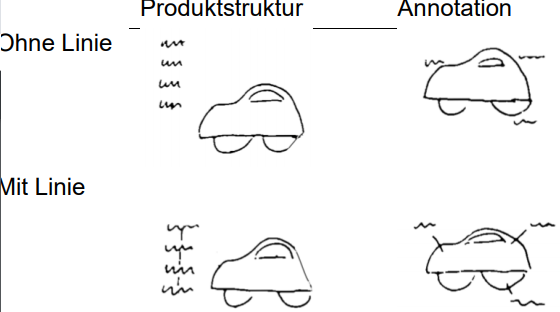
\includegraphics[width=.6\textwidth]{resources/analyse/brandenburg_uv.png}
	\caption{Darstellungsformen welche in der Studie evaluiert wurden. Quelle: \cite[S.~127]{Brandenburg2019}}
	\label{img:uv}
\end{figure}

Auf Abbildung 3.2 linke Seite, ist die getrennte Darstellung als Baumstruktur zu sehen. Die einzelnen Bauteile sind mit Verbindungslinien an Elternknoten welche eine Baugruppe bilden verbunden dargestellt. In der Studie wurde jeweils ein Begriff aus der Baumstruktur sowie ein Produktteil am Auto farblich grün hervorgehoben. 

Abbildung 3.2 rechte Seite, zeigt die Darstellung als Annotation. Hier wurde die Begriffe welche zu einer Baugruppe gehören durch eine grüne Einrahmung der jeweiligen Annotation von den anderen 
Annotationen farblich hervorgehoben.  

\begin{figure}[H]
	\centering
	\begin{minipage}{.5\textwidth}
		\centering
		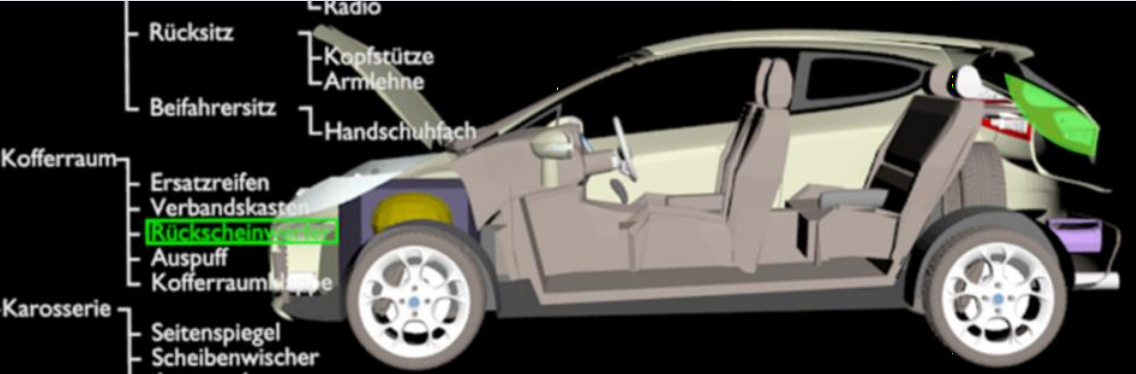
\includegraphics[width=.95\linewidth]{resources/analyse/baumstruktur.png}
		\label{fig:baum}
	\end{minipage}%
	\begin{minipage}{.5\textwidth}
		\centering
		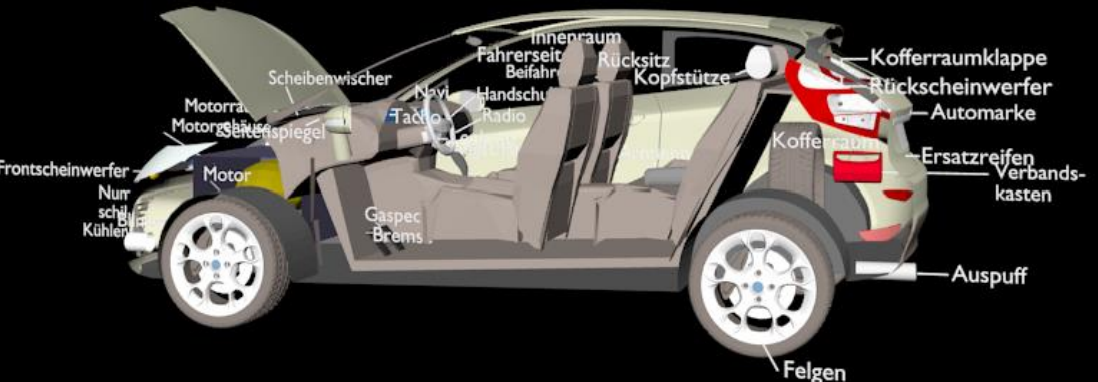
\includegraphics[width=.95\linewidth]{resources/analyse/annotation.png}
		\label{fig:annotation}
	\end{minipage}
\caption{Unterschiedliche Darstellungsformen - Links: Darstellung als Baumstruktur getrennt vom Produkt. Quelle: \cite[S.~127]{Brandenburg2019} Rechts: Darstellung als Annotation, am jeweiligen Produktteil. Quelle: \cite[S.~128]{Brandenburg2019}}
\label{img:versuchAbbildung}
\end{figure}

Abbildung \ref{img:aufgabenbeschreibung} zeigt die Aufgabenstellungen welche von den Versuchspersonen gelöst werden mussten:

\begin{figure}[H]
	\centering 
	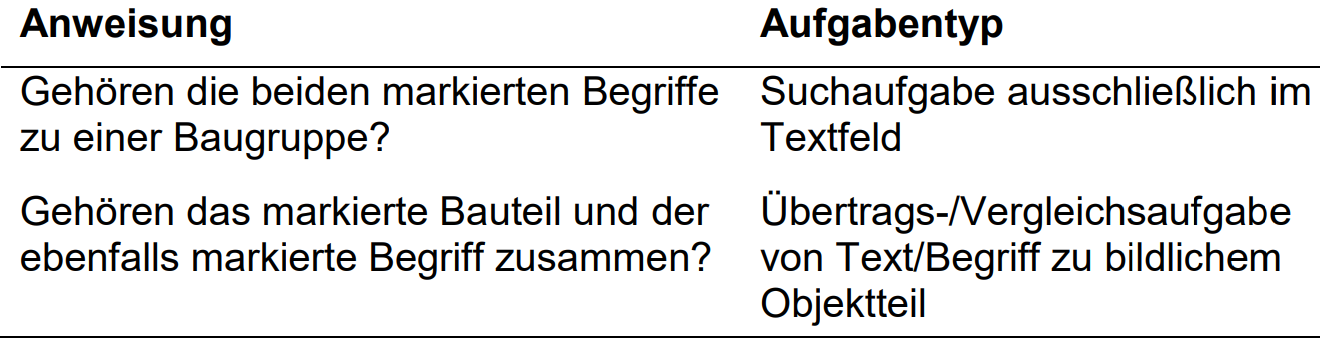
\includegraphics[width=.6\textwidth]{resources/analyse/brandenburg_aufgabentypen.png}
	\caption{Aufgabenbeschreibungen - Suche und Vergleichsaufgaben. Quelle: \cite[S.~132]{Brandenburg2019}}
	\label{img:aufgabenbeschreibung}
\end{figure}

Im Ergebnis dieser Studie konnten die Effekte beider Darstellungsformen auf die jeweiligen Aufgabentypen haben, welche von \citeauthor{Polys2007} in \cite{Polys2007} beschreiben werden, bestätigt werden.
Des weiteren hat sich in dieser Studie herausgestellt dass Annotationen welche mit einer Verbindungslinie dargestellt werden welches Text mit entsprechendem Produktteil verbindet 
zur effizienteren Lösung der Aufgabe beitragen.Quelle: \cite[S.~135]{Brandenburg2019}

\section{Zeigen und Auswählen in AR Benutzeroberflächen} \label{pointer_section}

In diesem Abschnitt werden Grundlagen für das zeigen und Auswählen in Virtuellen Umgebungen behandelt, sowie einige aktuelle Arbeiten 
zu diesem Thema näher betrachtet. 

Der digitale Prototyp soll auf ein Touchscreen Bildschirmoberfläche eines Smartphones genutzt werden.
\citeauthor{Ortega2016} beschreiben folgende grundlegende Probleme welche bei Interaktionen auf diesen Oberflächen auftreten können und daher beachtet werden sollten:  
Dadurch dass Interaktionen mit dem direkten Berühren des Bildschirmes stattfinden fehlt bei Touch Oberflächen das Drüber schweben (engl. Hover) bevor eine Aktion durch das Klicken der Maus Taste bestätigt wird. 
Dadurch dass der Finger auf den Bildschirm aufgelegt wird, besteht das Problem der Verdeckung. Zudem muss mit stark variierender Sinn für Präzision gerechnet werden. Weiter ordnen \cite[S.~205]{Ortega2016} Ansätze 
für die Behandlung dieser Probleme in zwei Gruppen ein: Die erste Gruppe behandelt diese Probleme in der Gestaltung der Benutzeroberfläche. Während in der zweiten Gruppe für die Lösung dieser Probleme, die Intension 
der Nutzers untersucht wird und die Interaktion entsprechend ausgeführt wird. \cite[S.~205]{Ortega2016}

Die Aufgabe ein Objekten in virtuellen Umgebungen auszuwählen, setzt sich aus einer Komposition dreier Teilaufgaben zusammen welche jeweils unterschiedlich umgesetzt werden können. 
Diese Teilaufgaben werden in \cite[S.~12]{Bowman1999} \cite[S.~150]{Bowman2011} als folgende vorgestellt: 

\begin{itemize}
\item \textit{Andeutung der Selektion eines Objektes (engl. Indication of object).} Dem Nutzer wird die Möglichkeit gegeben auf ein Objekt oder auf ein Bereich zu zeigen welches ausgewählt werden soll.
\item \textit{Bestätigen der Auswahl (engl. Confirmation of selection bzw. Indication to select).} Es werden Techniken zur Verfügung gestellt womit der Nutzer sein Auswahl bestätigen kann. 
\item \textit{Rückmeldung (engl. Feedback).} Die Bestätigung der Auswahl wird vom System bestätigt. 
\end{itemize}

Abbildung \ref{img:auswahluebersicht} stellt diese Teilaufgaben in einer Übersicht dar und zeigt einige Beispiele wie diese auf unterschiedlicher weise umgesetzt werden können. 

\begin{figure}[H]
	\centering 
	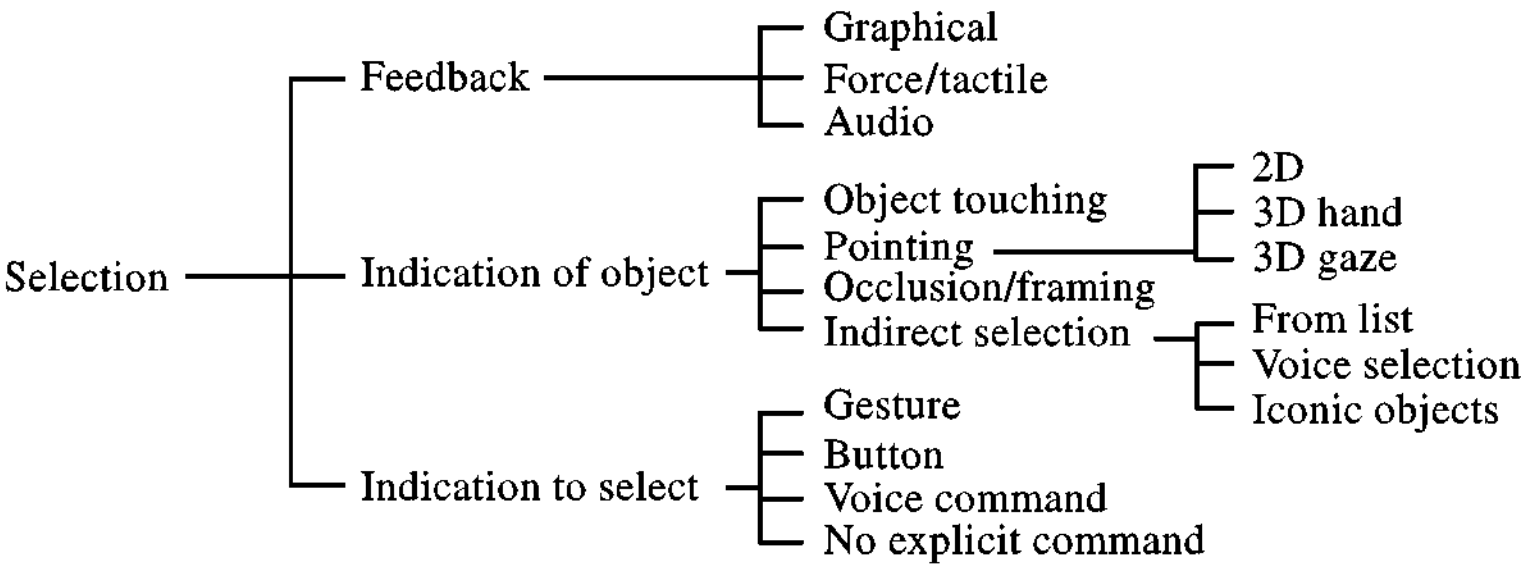
\includegraphics[width=.8\textwidth]{resources/analyse/Selection_uebersicht.png}
	\caption{Klassifikation von Auswahltechniken. Quelle: \cite[S.~12]{Bowman1999}}
	\label{img:auswahluebersicht}
\end{figure}

Beispielsweise kann das Andeuten einer Selektion durch die Auswahl in einer Listenansicht, durch Sprachbefehle oder durch das Zeigen umgesetzt werden. 
Ein Technik für das Zeigen stellt das Ray-Casting dar. Mit dieser Technik wird ausgehend von einer Startposition, in eine Richtung in welche gezeigt wird, ein Strahl 
ausgesendet welches Objekte in der Umgebung treffen kann. Dabei werden Schnittpunkte dieser Strahl mit Objekten aus der Umgebung verglichen und das Objekt    

\citeauthor{Bowman2011} bezeichnet das Zeigen durch Ray-Casting als eines der einfachsten und effektivsten Techniken für das Auswählen in virtuellen Umgebungen für Anwendungsfälle in welchen auf Objekte aus 
naher Distanz gezeigt wird.\cite[S.~153]{Bowman2011}

\citeauthor{Vincent2013} vergleichen in eine Studie zwei unterschiedliche Ansätze für das Zeigen zum Auswählen von Stellen auf planaren Oberflächen. 
Die Studie vergleicht folgende zwei Ansätze mit Anwendung auf zwei unterschiedlichen mobilen Endgeräten - Einem Tablet und einem Smartphone: 

\begin{itemize}
\item{Das Zeigen durch eine in der Mitte des Bildschirm fixierten Fadenkreuzes, diesen Ansatz bezeichnen \citeauthor{Vincent2013} als \textit{Crosshair}. Bei dieser Methode 
befindet sich auf der Mitte des Bildschirmes ein Fadenkreuz. Ausgehend von dieser Stelle wird von der Anwendung ein Strahl in die Umgebung ausgesendet und 
kann Objekte in der Umgebung treffen. Der Nutzer kann auf bestimmte Stellen auf planaren Oberflächen zeigen indem er das Mobile Endgerät bewegt und mit dem Fadenkreuz
auf die Stelle anvisiert (Abbildung \ref{img:pointing_vergleich} (B).} 
\item{Bei der zweiten Methode hingegen, welches als \textit{Relative Pointing} bezeichnet wird, wird der Fadenkreuz auf die Oberfläche fixiert, auf welchem die Selektion stattfinden soll. Der Nutzer kann die Position des Fadenkreuzes durch das Wischen auf der 
	Touchscreen Oberfläche verändern (Abbildung \ref{img:pointing_vergleich} (C).}
\end{itemize}

Zusätzlich wird der Versuch mit dem Zufügen einer künstlich erzeugtem Registrierungs-jitter d. h. einer stark schwankenden Positionsänderung der virtuellen Objekte (Abbildung \ref{img:pointing_vergleich} (D)) wiederholt. 

\begin{figure}[H]
	\centering
	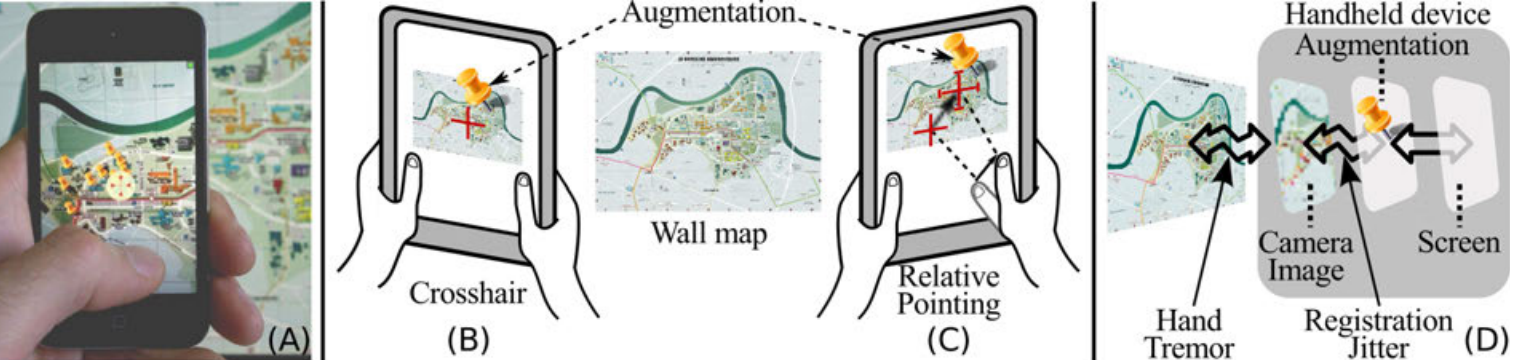
\includegraphics[width=.7\textwidth]{resources/analyse/Pointing_techniken.png}
	\caption{Darstellung zweier Ansätze für das Zeigen und Auswahl auf ebenen Oberflächen. Quelle: \cite{Vincent2013}}
	\label{img:pointing_vergleich}
\end{figure}

An der Studie nahmen 24 Versuchsteilnehmer teil und als Aufgabe musste auf einer Oberfläche, auf welchem kreise, welche ringförmig angeordnet sind ausgewählt werden. Die Kreise 
welche ausgewählt werden sollten sind jeweils blau hervorgehoben worden. Die Teilenehmer haben den Versuch von einer Entfernung aus ca. einem Meter Abstand ausgeführt. 

\begin{figure}[H]
	\centering
	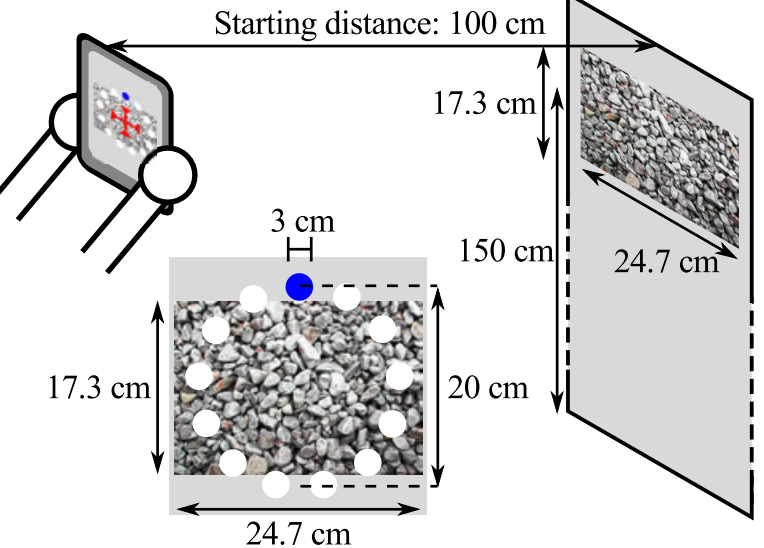
\includegraphics[width=.5\textwidth]{resources/analyse/versuchsaufbau.png}
	\caption{Versuchsaufbau - Vergleich Crossfade vs. Relative Pointing Quelle: \cite{Vincent2013}}
	\label{img:versuchsaufbau}
\end{figure}

Im Fazit dieser Studie kamen bei dieser Studie folgende Erkenntnissen: 

\begin{itemize}
\item{Der Ansatz \textit{Relativ Pointing} führt zu weniger Fehler (Verfehlen der Stelle welche ausgewählt werden soll).}
\item{Zusätzlicher Registirerungs-jitter beeinträchtigt die Genauigkeit der Auswahl mit \textit{Relativ Pointing} geringer.}
\item{Mit \textit{Relativ Pointing} zeigt sich ein geringer Unterschied hinsichtlich Genauigkeit und Dauer des Auswahlvorgangs und der verwendeten Endgerätes. Hingegen zeigt sich bei \textit{Crosshair} ein signifikanter Unterschied in welchem die Performance in beiden Punkten mit der Nutzung des Smartphones schlechter abschneidet.}
\end{itemize}

In einer weiteren Arbeit befasst sich \citeauthor{Vincent2014} mit dem Zeigen auf Oberflächen von drei dimensionalen Objekten. \cite[S.~92]{Vincent2014}

\begin{figure}[H]
	\centering
	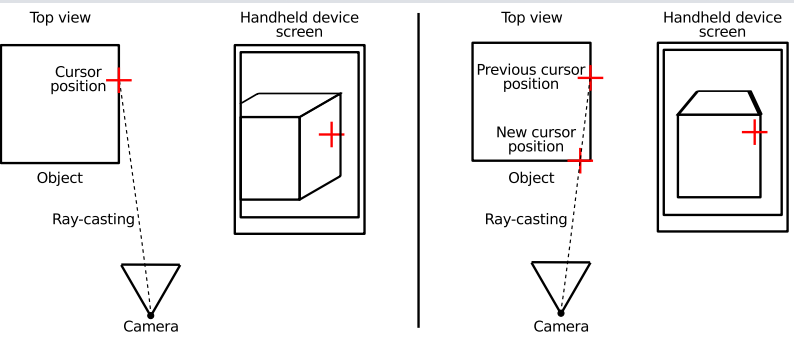
\includegraphics[width=.7\textwidth]{resources/analyse/pointing_3d.png}
	\caption{Relative Pointing auf der Oberfläche von 3D Objekten. Quelle: \cite[S.~84]{Vincent2014}}
	\label{img:pointing_auf3d}
\end{figure}

Bei der Anwendung des \textit{Relative Pointing} auf 3D Oberflächen macht \citeauthor{Vincent2014} auf einen Unterschied aufmerksam: Der Fadenkreuz bzw. der Zeiger kann durch die Struktur des
3D Objektes verdeckt werden oder durch ein Perspektivenwechsel der Kamera, sich nicht mehr im Sichtbereich befinden. Er schlägt für die Behandlung dieses Problems vor, mit Ray-Casting zu überprüfen, 
ob der Zeiger sich im nächsten Schnittpunkt des Ray-Cast befindet und ihn dort zu platzieren falls dieser an einem anderen Bereich befindet. Der Ray-Cast soll dabei ein virtuellen 3D Modell des Objektes treffen.
Als eine alternative dazu schlägt er vor, die Tiefen-Sensor der Kamera zu nutzen diesen Vorgang auf dem physischen Objekt durchzuführen zu können. \cite[S.~83]{Vincent2014}

\section{Immersive Product Improvement (IPI)} \label{ipi_section}

In diesem Abschnitt wird ein von \citeauthor{Kirschner2012} in \cite{Kirschner2012} vorgestellter methodischer Lösungsansatz für Open Innovation (zu dt. Offene Innovation) betrachtet und 
drei unterschiedliche Umsetzungsmöglichkeiten welche \citeauthor{Kirschner2012} vorstellt. 

Open Innovation beschreibt den Innovationsprozess eines Unternehmens, bei welcher interne sowie externe Ideen genutzt werden um diese in der Produktentwicklung umzusetzen und ihr Wissen weiterzuentwickeln. 
Im Gegensatz dazu gehen Impulse zur Innovation in Closed Innovation  lediglich von innerhalb des Unternehmens aus.\cite[S.~32]{Kirschner2012}

Die von \citeauthor{Kirschner2012} vorgestellte Methode setzt ein bereits existierendes Produkt voraus an welchem,  Nutzern,  Nutzungserfahrung sammeln und Verbesserungsbedarf feststellen. 
Diese sollen Nutzer dann als Verbesserungsvorschläge in Form von Kommentaren auf den Produkten, an den entsprechenden stellen anbringen können. Diese Verbesserungsvorschläge sollen dem Hersteller
bei der Überarbeitung der Produkte im Zuge der Modellpflege oder Nachfolgerplanung helfen. Abbildung \ref{img:ipimethode} veranschaulicht diese Methode. \cite[S.~122]{Kirschner2012}

\begin{figure}[H]
	\centering
	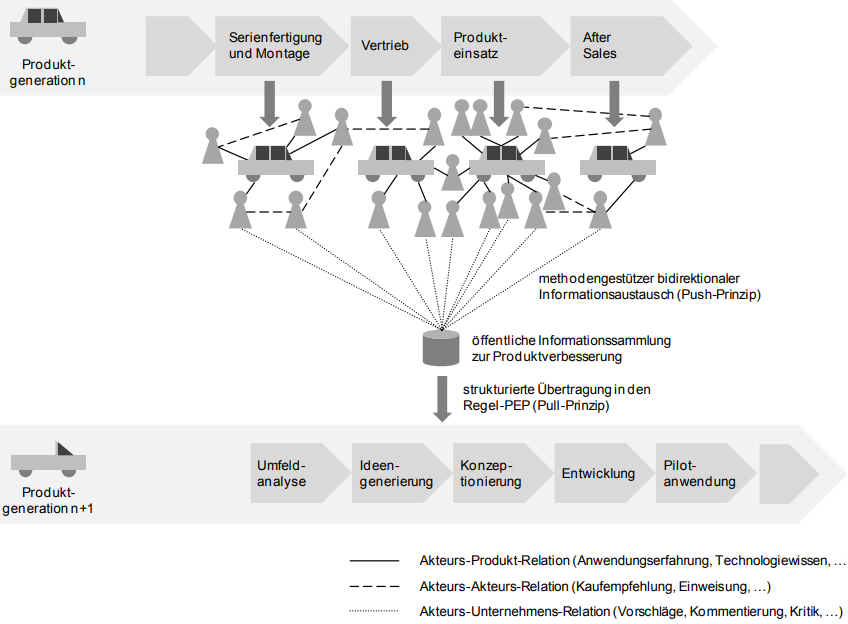
\includegraphics[width=1.0\textwidth]{resources/analyse/IPI_methode.png}
	\caption{Grobkonzept der IPI-Methode. Quelle:\cite[S.~128]{Kirschner2012}}
	\label{img:ipimethode}
\end{figure}

Als Tools für die Umsetzung dieser Methode stellt \citeauthor{Kirschner2012} drei Ansätze vor: Die pysische Umsetzung, bildzentrierten Umsetzung oder objektzentrierten Umsetzung (mit Augmented Reality). 

Mit der phyischen Umsetzung wird ein Exemplar des Produktes ausgestellt und Nutzer können Verbesserungsvorschläge durch das Anbringen von Notizzetteln auf dem Produkt abgeben. 
Dabei sollte nach \citeauthor{Kirschner2012}, darauf geachtet werden dass Notizzettel an Referenzpunkten (an der Stelle am Produkt welche mit dem Beitrag verknüpft ist) angebracht werden. Damit 
soll verhindert werden dass keine gleichen Beiträge für die gleiche Stelle am Produkt abgegeben werden. 

Die Vorteile dieser Umsetzung führt \citeauthor{Kirschner2012} auf, dass diese Methode den höchsten Grad an Immersion bietet, da ein einziges Produkt als  Nutzungs- und
Beitragsbasis verwendet wird. Zudem ist diese Methode kostengünstig und schnell einsetzbar und erfordert keine Serienproduktion. 
Die Nachteile dieser Umsetzung sind jedoch: Einschränkte Anzahl an teilnehmenden Nutzern sowie der Verzicht auf akteursinitiierte Teilnahme, eingeschränkte Skalierbarkeit und aufwendigere Auswertung mit potenziell 
höherer Fehlerquellen. Zudem wäre diese Methode bei länger laufender Einsatz personal bedingt überproportional teuer. \cite[S.~125]{Kirschner2012}

Beim bildzentrierten Ansatz werden Abbildungen des Produktes über eine Onlineplattform des Herstellers zur Verfügung gestellt. Die Nutzer haben die Möglichkeit auf über einer Listenansicht oder direkt auf der 
Abbildung des Produktes bestimmte Referenzpunkte auszuwählen und ein Kommentar dazu abzugeben. Bestehende Kommentare andere Nutzer einsehen und bewertet werden. Weiter können Nutzer bei Abgabe eines Kommentars
diesen thematisch zu einem vom Hersteller vorgegeben Kategorie einordnen. \cite[S.~127]{Kirschner2012}

Zu diesem Ansatz wurde \citeyear{Kirschner2011} von \citeauthor{Kirschner2011} eine Studie durchgeführt worin der Zugang zu Referenzpunkten am Produkt über Listen und Bildansicht verglichen wurde. Abbildung 
\ref{img:ipi_list_image} zeigt beide Ansichten. \cite{Kirschner2011}.

Die Studie wurde mit 48 Teilnehmern durchgeführt wobei die 24 Zugang mit Zugang über die Listenansicht Kommentare abgeben konnten und die anderen Teilnehmer über die Bildzugang. Die Teilnehmer hatten sieben Tage 
Zugang auf die Plattform um Kommentare abzugeben und bestehende Kommentare zu bewerten. 

\begin{figure}[H]
	\centering
	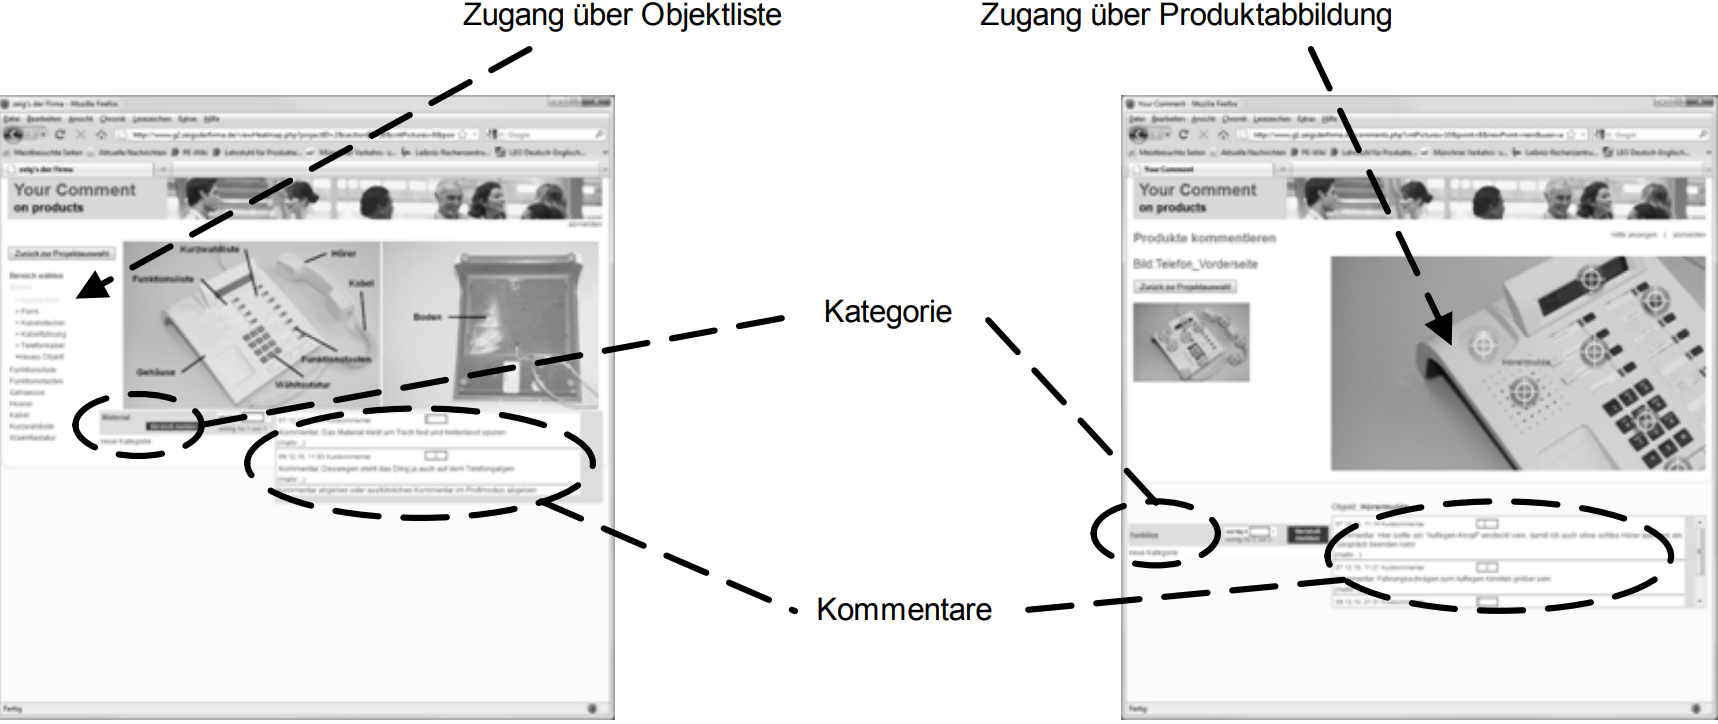
\includegraphics[width=1.0\textwidth]{resources/analyse/IPI_Vergleich_Listen_BildAnnotationeAnsicht.png}
	\caption{Online-Produktkommentierung über Listen- und Bildzugang. Quelle: \cite[S.~7]{Kirschner2011}}
	\label{img:ipi_list_image}
\end{figure}

Im Ergebnis dieser Studie kam heraus dass über Bildzugang deutlich mehr Kommentare erstellt werden gegenüber dem Zugang ober Listenansicht. Auch die Anzahl an Bewertungen (auf Abbildung \ref{img:ergebnisse_listen_bildzugang} sind diese mit ``threads`` bezeichnet) ist ein deutlicher Unterschied zu erkennen. Die Autoren vermuten dass dieser deutliche Unterschied durch die 
zusätzliche kognitive Beanspruchung verbunden ist, die benötigt wird um die textuelle Information aus der Liste mit den entsprechenden Stellen des Produktes zu verbinden.

\begin{figure}[H]
	\centering
	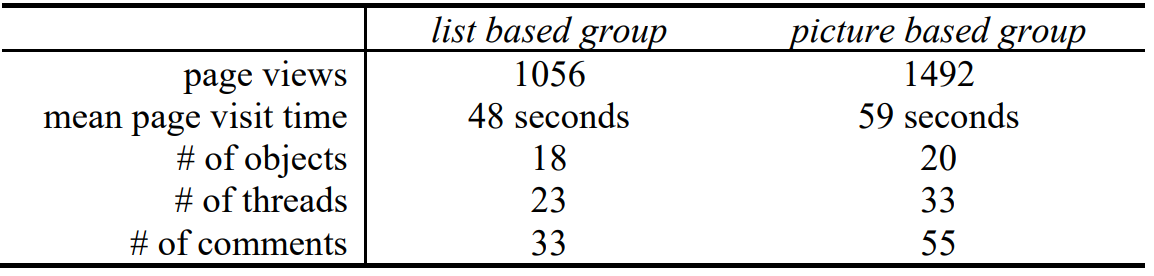
\includegraphics[width=.8\textwidth]{resources/analyse/results_list_picture_based.png}
	\caption{Ergebnisse der Erhebung - Vergleich Liste vs. Bildzugang. Quelle: \cite[S.~7]{Kirschner2011}}
	\label{img:ergebnisse_listen_bildzugang}
\end{figure}

Mit der objektzentrierten Ansatz sollen Nutzer die Möglichkeit haben über die Nutzung eines mobilen Endgerätes das Produkt zu betrachten. 
Durch entsprechende Objekterkennungsmechanismen das Produkt erkannt und bestehende Kommentare auf dem Produkt an entsprechenden Stellen dargestellt werden können.
Dies erfordere die Umsetzung mit Augmented Reality.\cite[S.~135]{Kirschner2012}

\begin{figure}[H]
	\centering
	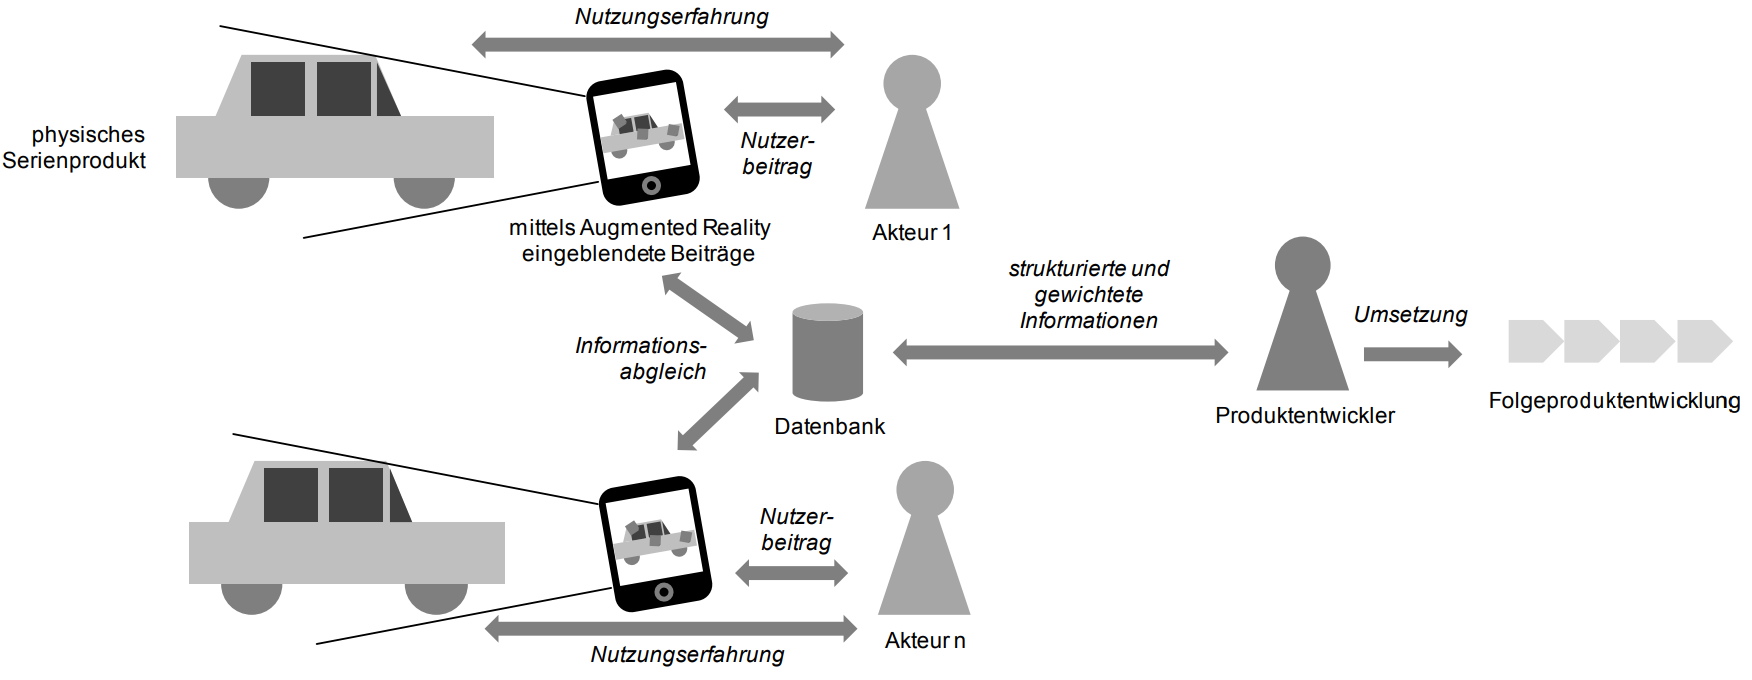
\includegraphics[width=1.0\textwidth]{resources/analyse/IPI_Objektzentriert.png}
	\caption{Informationsfluss in der objektzentrierten IPI-Umsetzung. Quelle:\cite[S.~135]{Kirschner2012}}
	\label{img:objekt_centered_ipi}
\end{figure}

Als Vorteile diesen Ansatzes beschreibt \citeauthor{Kirschner2012}: Dass das Produkt automatisch erkannt werden kann und er Nutzer das Produktbild nicht auswählen muss. Zudem biete dieser Ansatz im Vergleich zum 
bildzentrierten Ansatz einen höheren Grand an Immersion. Als Nachteile beschreibt er dass ein erhöhter Maß an technischen Aufwand für die Umsetzung erforderlich sei und zum aktuellen Stand der Technik die 
Stabilität der technischen Umsetzung noch nicht gewährleistet sei. Weiter beschreibt er dass das Produkt physisch oder zumindest visuell sich vor dem Nutzer befinden müsse und somit ein Teil der Beiträge wegfallen würde.\cite[S.~130]{Kirschner2012}








 \clearpage
\chapter{Konzeption}

In diesem Kapitel wird die Konzeption des Gesamtsystems beschrieben. Es wird die Nutzungskontextanalyse beschrieben, welches als Grundlage und Vorbereitung für die anschließende Anforderungsanalyse diente. Die Anforderungsanalyse in welcher, im Rahmen eines Kreativ Workshops, Anwendungsfälle für das zu konzipierende System erarbeitet wurden, wird erläutert. Abschließend wird ein Entwurf der Anwendung beschrieben.

\section{Nutzungskontextanalyse}

% Aktuelle Problemlösungstrategien? Bewertungen auf Online Portalen, Blogs, Interessengruppen, Reklamationen, Technischer Support
Aktuelle Lösungen für die Abgabe von Feedbacks zu Produkten erfolgt oft ohne den Einsatz von Augmented Reality. Diese erfolgen 
oft als Bewertungen in Online Einkaufsportalen, Blog Beiträgen, durch den Austausch in Interessengruppen oder über direkten Kontakt zum Hersteller.

Bei Bewertungen in Onlineportalen, in Blog Beiträgen oder auch bei direktem Kontakt zum Hersteller (z.Bsp. durch E-Mail), haben Kunden die Möglichkeit 
Ihre Feedbacks schriftlich zu beschreiben und mit Bildern oder Videos zu ergänzen. Bei solchen Beschreibungen kommt es jedoch manchmal vor dass 
nicht immer klar hervorgeht zu welcher Stelle oder zu welches Teil am Produkt sich die Beschreibung bezieht. Informationen über die Umgebung in welchem das Produkt 
verwendet wird, geht aus solchen Beschreibungen auch nicht immer hervor. Zudem ist nicht ohne Aufwand möglich direkt zu erkennen an welchen Stellen eines Produktes 
Feedbacks häufen.

Bei Interessengruppen in welchen Nutzer von bestimmten Produkten, sich räumlich zusammentreffen um Erfahrungen auszutauschen wie z.Bsp. zu Hausaltprodukten, Modellflugzeugen, VR Headsets usw., 
haben die Nutzer die Möglichkeit Ihre Ideen genauer zu beschreiben. 
Bei solchen Treffen haben die Nutzer die Möglichkeit mit Bezugnahme auf die Stellen am Produkt und dem Kontext ihrer Umgebung Feedback zum Produkt zu geben. Das Problem bei dieser Art der Rückmeldungen ist jedoch dessen eingrenzte Reichweite. Zudem werden Inhalte welche in solchen Treffen diskutiert wurden oft nicht ausreichend dokumentiert.  

Auf Basis der im Kapitel \ref{CapterFundamentals} behandelten Grundlagen und der Nutzungskontextanalyse wurde eine erste Skizze des Gesamtsystems entworfen in welcher, 
Funktionale wie Nicht-Funktionale Anforderungen an das zu konzipierende System skizziert wird (siehe Abbildung \ref{img:sysstem_sketch}).

\begin{figure}[H]
	\centering
	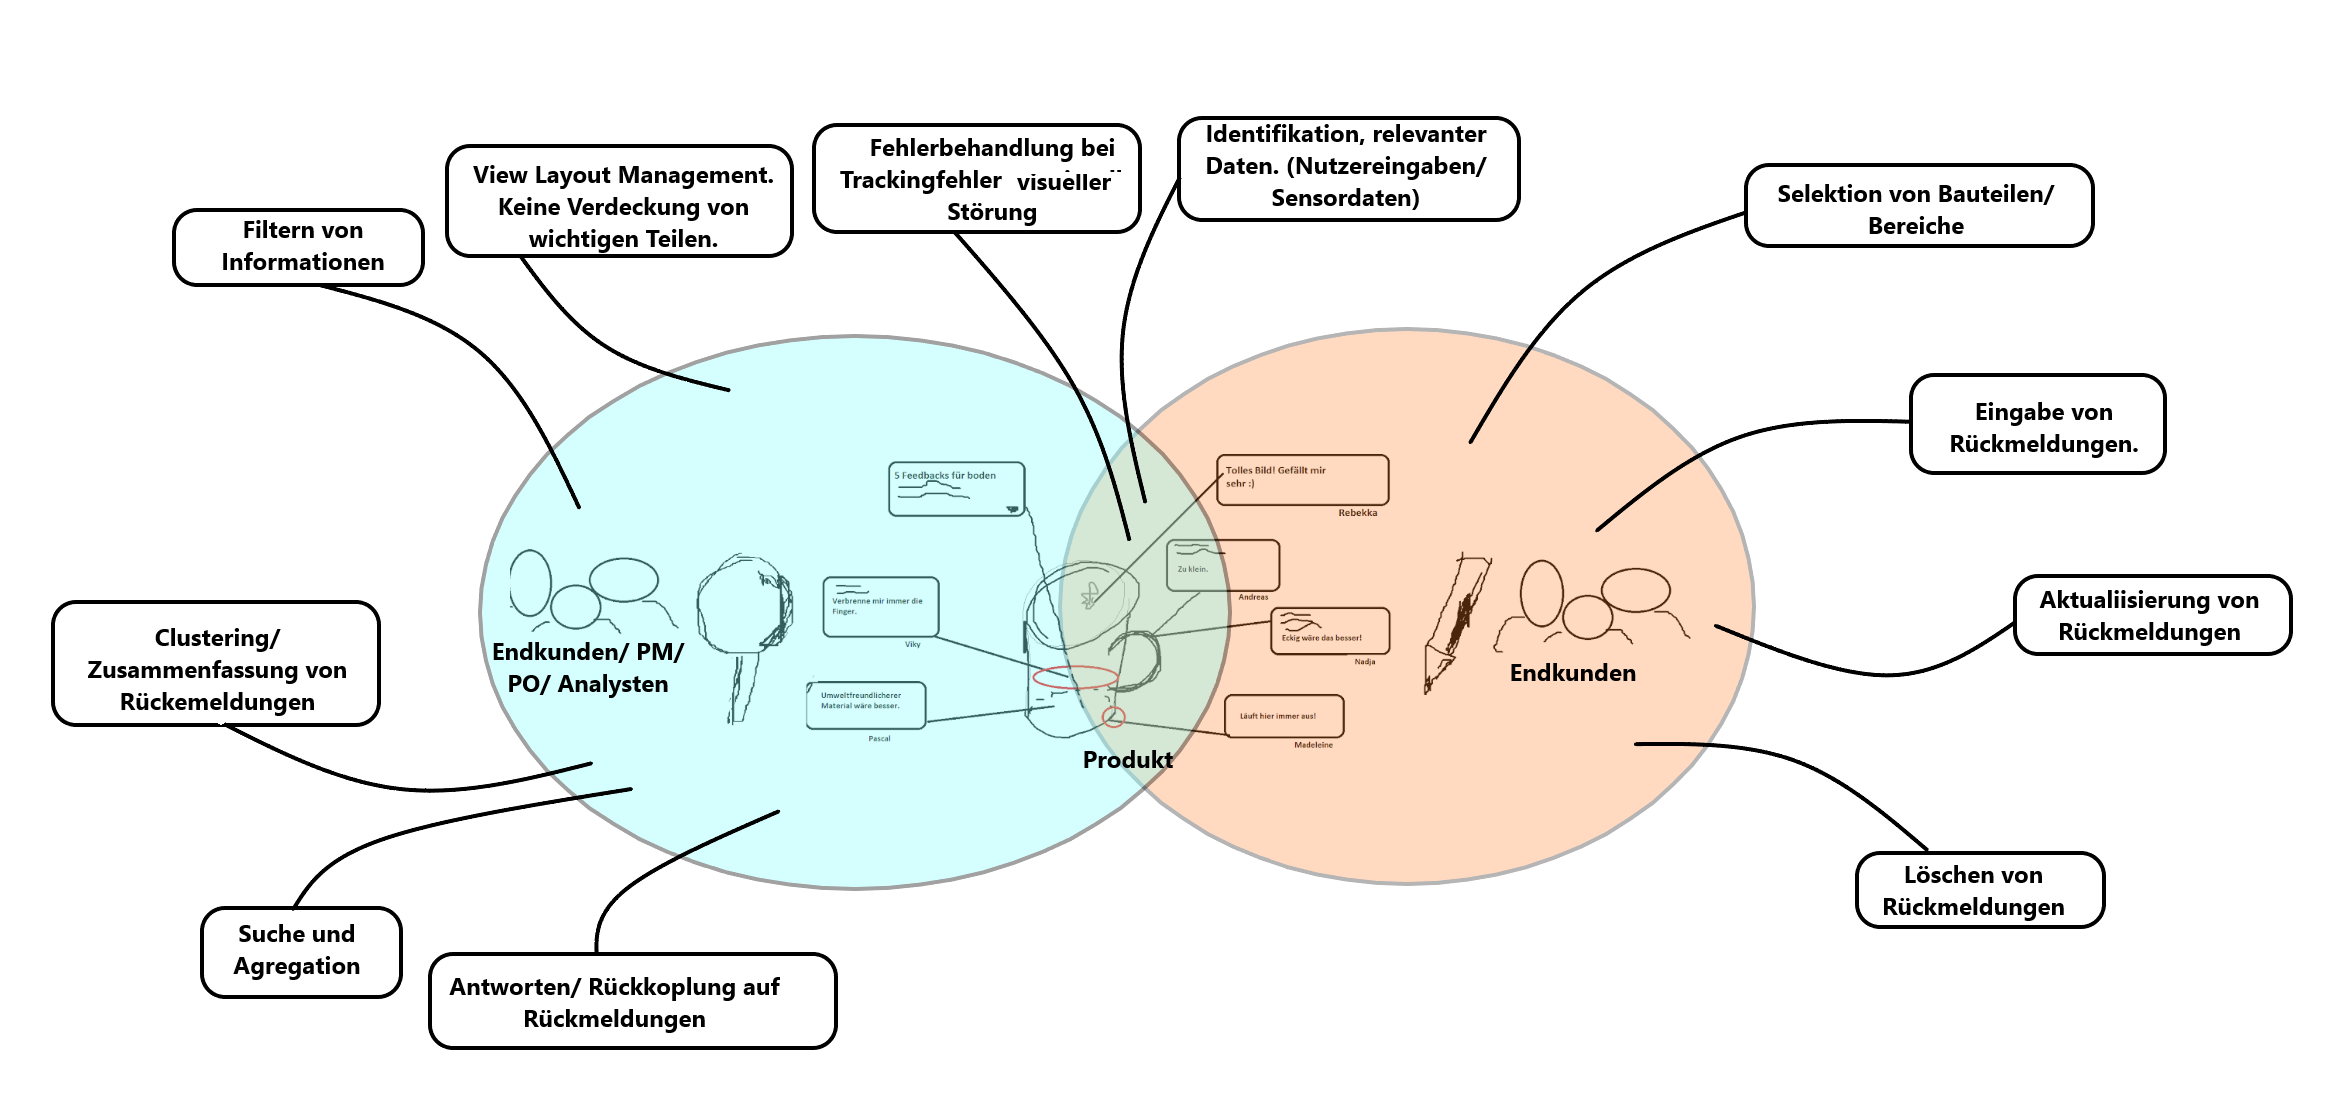
\includegraphics[width=1.0\textwidth]{resources/conception/skizze_gesamtsystem.png}
	\caption{Skizze des Gesamtsystems als erster Entwurf \\Quelle: Eigene Darstellung}
	\label{img:sysstem_sketch}
\end{figure}

Dieses Skizze sollte die Projektidee begreifbarer machen und als grobe Orientierung bei der Anforderungsanalyse dienen.

\section{Anforderungsanalyse}

Die Anforderungsanalyse wurde im Rahmen eines Kreativ Workshops durchgeführt. Ziel des Workshops war es Die Nutzer für das zu konzipierende System zu identifizieren und deren Eigenschaften und Bedürfnisse 
zu analysieren. 

% Vorbereitung
Das Workshop fand am dritten Juli, am Fraunhofer IPK in Berlin statt. Zur Vorbereitung wurde in einem zuvor für diesen Workshop gebuchten, Besprechungsraum, einzelne Stationen \footnote{z.Bsp.: Aufstellung eines Pinnwand für die Erstellung eines Affinitätsdiagrammes, Abbildungen von Personen für die Erstellung von Personas usw.} für die am Workshop durchzuführenden Aktivitäten vorbereitet. 
Zunächst wurden die Teilnehmer begrüßt und für die Teilnahme am Workshop bedankt. Anschließend wurde der Anlass und der Ablauf des Workshop vorgestellt. 

%Durchführung
Mit Hilfe einer kurzen PowerPoint Präsentation wurde die Projektidee vorgestellt und anhand der groben Skizze des zu konzipierenden Systems (Abbildung \ref{img:sysstem_sketch}) verdeutlicht. 
Anschließend fand eine Frage- Antwort Runde statt, welches die Möglichkeit gab, Rückfragen zu stellen und somit sicherzustellen, dass die Projektidee von allen Teilnehmer gleichermaßen verstanden wurde. 

Nach der Vorstellung der Projektidee fand ein Brainstorming statt, dessen Ergebnis in ein Affinitätsdiagramm festgehalten wurden. 
Im gewöhnlichen Vorgang für die Erstellung von Affinitätsdiagramme, schreiben Teilnehmer Ideen auf Kärtchen, welche zunächst unsortiert auf ein Pinnwand geheftet werden. 
Anschließend werden die Ideen, gemeinsam besprochen und in Gruppen bzw. Untergruppen sortiert. In dem stattgefundenen Workshop wurden die Gruppen jedoch im voraus vorgegeben. 

Es sollten Ideen für die Beantwortung folgender Fragen gesammelt werden: 

\begin{itemize}
	\item Wer sind die Nutzer? (Rolle, Erfahrungsstand,  Lebensstil/ Lebenskontext)
	\item Was sind aktuelle Problemlösungsstrategien der Nutzer?
	\item Was sind die Ziele der Nutzer?
	\item Wo liegen die Schmerzpunkte mit aktuellen Lösungstretarien?
\end{itemize}\label{list:AffiDiagramm}

Den Teilnehmern wurde 15 Mintuten Zeit für ein Brainstorming gegeben, indem Ideen zu den, oben genannten Fragen, auf Kärtchen aufschreiben wurden.
Folgende Ideen sind in dabei entstanden (Eine Abbildung des entstandenen Affinitätsdiagramm befindet sich im Anhang [Referenz darauf]): 

\vspace{5mm}
\textbf{Nutzer: } 
Technik Nerd, Produkt Entwickler, Werbeagentur, Unzufriedene, Unerfahrene, Gewerbliche Nutzer/ Laborpersonal, Endkunde, Qualitätsprüfung eines Produkts (Vorgesetzter), Lagerpersonal

\vspace{5mm}
\textbf{Aktuelle Problemlösungsstrategien} 
Email, Chat, Web-Portale, Telefonsupport, Vergleich von Käuferbewertungen

\vspace{5mm}
\textbf{Ziele der Nutzer: } 
Nächstes Produkt sollte besser sein, Eigenes Design, Fehleranfälligkeit beseitigen, Informationen vor dem Kauf, Hilfreiche Bewertungen finden und verstehen, Ersatzteile beschaffen, Lösungen aus dem Nutzerkreis bereitstellen, Infos in Form: Kurzer Beschreibungen/ Kontakt Informationen des Verantwortlichen, Anleitungen, Reklamation Technischer Dokumentationen (Montageanleitung)

\vspace{5mm}
\textbf{Pain-Points: } 
Komplizierte Beschreibung der Umgebung/ Use Case, Zustand der Bearbeitung unbekannt, Fehlerbehebung meines Produktes, Produkt wird nicht wie vorgesehen (geplant) genutzt und funktioniert daher nicht richtig (Vorstellung eines möglichen neuen Anwendungsfalles), Lange Wartezeiten auf Antwort, Bessere Kommunikation zwischen Abteilungen

%Durchführung %Aufbau / Einleitung / Affinitätsdiagram / Personas / Szenarien

%Personas Tabelle

%Name/ Alter / Rolle /Aktuelle Problemlösung / Pain Points

% User Stories


\textbf{User Stories}


%\begin{center}
	\begin{table}[H]
	\caption{User Stories}
	\resizebox{\textwidth}{!}{
	\begin{tabular}{ | c | c | c |c |c |}
		\hline
		\thead{Nr.} & \thead{Als} & \thead{abgeleitet \\ aus \\ Persona} &	\thead{möchte ich} & \thead{damit} \\
		\hline
		10 &  \makecell{Endkunde} & \makecell{Timo} & \makecell{neue Anwendungsfälle \\direkt am Produkt-Teil\\ beschreiben können} &  \makecell{ich bei meiner Beschreibung\\ implizit einen Bezug\\
			zu einer bestimmten\\ Stelle am Produkt\\ herstellen kann} \\
		\hline
		20 &  \makecell{Endkunde} & \makecell{Timo} & \makecell{Ergänzende Anleitungen direkt\\ am Produkt am Produkt Teil\\ oder Stellen ansehen können} &  \makecell{ich mir ergänzende Bemerkungen \\und Anleitungen
			direkt an der \\ betreffenden Stelle ansehen kann
} \\
		\hline
		30 &  \makecell{Endkunde} & \makecell{Timo} & \makecell{Anleitungen zu spezifischen\\ Stellen am Produkt \\beschreiben können} &  \makecell{mir die Bezugnahme zur \\ betreffenden Stelle
			am Produkt\\ erleichtert wird und meine \\Anleitungen
			besser von anderen \\verstanden werden} \\
		\hline
		31 &  \makecell{Endkunde)}  & \makecell{Svenja, \\ Timo, \\ Felix} & \makecell{ein bestimmtes Teil an einem\\
			physischen Produkt auswählen\\
			können
} &  \makecell{ich bezugnehmend auf das ausgewählte\\ Teil
			Aktionen ausführen kann.\\ (z. Bsp.: eine
			Rückmeldung abgeben)}\\
		\hline
		32 &  \makecell{Endkunde}  & \makecell{Svenja, \\ Timo, \\ Felix} & \makecell{eine von mir abgegebene\\
			Rückmeldung auswählen können} &  \makecell{damit ich diese Rückmeldung oder den\\
			Bezugspunkt auf dem physischen Produkt auf das\\
			sich die Rückmeldung bezieht verändern oder\\
			löschen kann}\\
		\hline
		33 &  \makecell{Endkunde}  & \makecell{Svenja, \\ Timo, \\ Felix} & \makecell{die Beschreibung auf einer von mir\\
			abgegebenen Rückmeldung verändern\\
			können.} &  \makecell{ich eine Nachträgliche Korrektur oder Ergänzung\\
			vornehmen zu kann.
}\\
		\hline
		34 &  \makecell{Endkunde}  & \makecell{Svenja, \\ Timo, \\ Felix} & \makecell{den Bezugspunkt (Produkt-Teil oder\\
			bestimmte Stelle auf einem\\
			Produkt-Teil) auf die ein von mir\\
			erstellte Rückmeldung sich bezieht\\
			verändern können.
} &  \makecell{ich eine Nachträgliche Korrektur oder Ergänzung\\
			vornehmen zu kann.
}\\
		\hline
		35 &  \makecell{Endkunde}  & \makecell{Svenja, \\ Timo, \\ Felix} & \makecell{eine von mir erstellte Rückmeldung\\
			löschen können} &  \makecell{ich eine obsolete, redundante oder versehentlich\\
			erstellte Rückmeldung wieder entfernen kann}\\
		\hline
		40 &  \makecell{Endkunde}  & \makecell{Svenja} & \makecell{schnell und unkompliziert\\
			Feedbacks zu Produkt Teile od. Stellen\\
			abgeben können.} &  \makecell{ich auch Feedbacks beiläufig abgeben kann.}\\
		\hline	
		50 &  \makecell{Endkunde}  & \makecell{Svenja, \\ Timo, \\ Felix} & \makecell{möchte ich Bewertungen zu einem\\
			Produkt, am Produkt ansehen können} &  \makecell{ich mich vor dem Kauf eines Produktes genauer\\
			erkundigen kann und mir vor allem für mich\\
			wichtigen stellen am Produkt besser beurteilen\\
			kann
}\\
		\hline	
		60 &  \makecell{Endkunde}  & \makecell{Svenja, \\ Timo, \\ Felix} & \makecell{möchte ich Kontaktinformationen zu\\
			Verantwortlichen Personen sehen\\
			können.} &  \makecell{ich direkt Kontakt zu dieser Person aufnehmen\\
			kann.}\\
		\hline	
		70 &  \makecell{Endkunde}  & \makecell{Timo} & \makecell{möchte ich den Wunsch äußern\\
			können, dass der Hersteller über mein\\
			Feedback informiert wird} &  \makecell{ich sichergehen kann dass mein Feedback\\
			zeitnah vom Hersteller wahrgenommen wird}\\
		\hline	
		80 &  \makecell{Endkunde}  & \makecell{Timo} & \makecell{möchte ich bei Abgabe eines Feedbacks,\\ den
			Einfluss auf mein Geschäft\\
			beschreiben können} &  \makecell{damit ich dem Hersteller des Produktes\\ ein besseres Verständnis über den Ausmaßes ermöglichen\\ kann und dieser den im Feedback beschriebenen\\ Sachverhalt entsprechend beurteilen und priorisieren kann }\\
		\hline	
\end{tabular}}
\end{table}
%\end{center}

%	20 &  \makecell{Geschäftskunde \\ (gewerblich \\ nutzender \\ Endkunde)}  & \makecell{Svenja, \\ Timo, \\ Felix} & \makecell{Text text text  \\ text text text text text} &  \makecell{Text text text  \\ text text text text text} \\
%\hline


\section{Entwurf}

\subsection{Szeanrien}
\subsection{Low-Fidelity-Prototyp}
\subsection{Konzeptioneller Entwurf und Klassendiagramme}

Systemkomponente

Entity Relationship Diagramm (ERM)


Klassendiagramm \clearpage
\chapter{Implementierung}\label{implementation}

In diesem Kapitel wird der Vorgang der Implementierung des digitalen Prototypen erläutert. Zunächst wird ein kurzer Einblick über die verwendete Spiele Enigen Unity gegeben und wichtige Komponente erklärt. 
Anschließend wird die Auswahl der Traking Framework sowie die verwendete Traking Methode erläutert. Es wird die Wahl der passenden Zeige und Auswahl Methode erläutert sowie die Verarbeitung der 
Eingabedaten über die Touchscreen Oberfläche an mit einer Flussdiagramm veranschaulicht. Abschließend wird er digitale Prototyp vorgestellt und die Vorbereitung des Prototypen auf die Studie erklärt. 

\section{Entwicklungsumgebung}

\subsection{Game Engine}

Unity ist ein Spieleengine des Unternehmens Unity Technologies und stellt eine Entwicklungsumgebung vorwiegend für Spiele dar. Jedoch hat sich Unity seither 
zu einem vielseitigen Werkzeug auch in anderen Bereichen als der Spieleenwticklung (z. B. im Bereich der Industrie) entwickelt. 
Unity ermöglicht die Entiwcklung von Anwendung für über 25 Plattformen darunter Plattformen für mobile Endgeräte wie Android oder iOS.

Zu den für die Verständnis dieser Arbeit wichtigen Komponente der Unity Umgebung zählen Szenen, Komponente, Prefabs sowie GameObjekts. Folgend werden diese kurz erläutert:

\textit{Szenen:} In Unity ist die Entwicklung in Szenen organisiert. Jede Szene besteht aus einem Szenengraph. Dieser Graph enthält wiederum weiter Objekte wie z. B. Game Objekte. 

\textit{GameObejects:} Game Objekte stellen in Unity Objekte dar wie zum Beipsiel eine Lichtquelle, eine Audioquelle oder eine geometrische Form wie ein Würfel. Game Objekte erhalten Eigenschaften durch 
Hinzufügen von Komponente. \cite{Unity}\\

\textit{Komponente:} Komponente geben Game Obejekten Eigenschaften und steuern diese. Eine Komponente kann zum Beispiel ein Material sein welches gewisse Eigenschaften wie eine Farbe oder Textur hat. 
Durch das hinzufügen eines Skriptes als Komponente an ein Game Objekt kann dieses darüber gesteuert werden.\cite{Unity}\\

\textit{Prefabs:} In Unity können Game Obejekte vorgefertigt sodass diese nicht zur Laufzeit erstellt werden müssen. Dies vorgefertigten Game Objekte sind so genannte Prefabs welche. Es kann zur Laufzeit eine Instanz eines Prefabs erzeugt werden.\cite{Unity}\\

Zu den unterstützten Programmiersprachen in Unity zählen Java Script und C\#. Für die Entwicklung des digitalen Prototypen wird die Programmiersprache C\# verwendet und die Visual Studio IDE der Firma Microsoft genutzt. 

\subsection{Tracking}

% Am besten geeignet: Kombination aus Modellbasiertes Tracking mit Verwendung eines CAD Modell des Produktes und Modellfreis Tracking damit das Traking aufrecht erhalten bleibt auch wenn nur Teile des Produktes im Sichtbereich der Kamera ist. 
% Ausprobiert wurde Model Tracking mit Vuforia sowie VisionLib. Vuforia hat nicht geklappt. VisionLib hat sehr gut geklappt mit Testlizez am Beispiel Model. Mit unterschiedlicher Beleuchtung, mit Bewegung des Models. 
% Jedoch war Lizenzverlängerung nicht möglich da Lizenztool für die Generierung von Lizenzen zur akademischen Nutzung nur für IOS möglich war. 

Da die Applikation verwendet werden soll um Produkte mit virtuellen Informationen war es naheliegend ein Traking Verfahren zu wählen welches für die Registrierung die Produkte selbst nutzen kann: Modellbasiertes Tracking mit Verwendung von 3D CAD Modell des Produktes. 
Hierzu wurden zwei Framework in Betracht gezogen und ausprobiert. Das AR Tracking Framework der Vuforia der Firma PTC sowie VisionLib der Firma Visometry GmbH. 

Zu dem Vorteilen von Vuforia zählten, dass Vuforia als Framework in Unity bereits integriert ist sowie die Ermöglichung eine Kombination von modellbasieten und modellfreies Tracking zu verwenden. 
Mit Vufofia kann wahlweise für modellfreies Tracking die Frameworks ARCore für Android Endgeräte oder ARKit für iOS Endgeräte verwendet werden. 

Auf der anderen Seite waren die Vorteile des VisionLib Framework die dass dieses, sich durch eine schlanke SDK schnell in Unity integrieren lässt. Zudem erschien das Tracking von 3D Modellen mit VisionLib stabil und wenig empfindlich gegen 
unterschiedlichen Lichtverhältnissen, Bewegungen des Modells sowie z. B. geringer Textur des Modells zu sein. \footnote{Beschreibung des VisionLib Framework: https://visionlib.com/awe/ [Letzter Zugriff: 07.09.2019]}

Das Tracking mit dem VisionLib Framework wurde am Beispiel eines vom Hersteller bereitgestellten Spielzeugauto aus Papier getestet. Nach einer Kalibrierung der Kamera konnte das Tracking getestet werden. Das Spielzeugauto wurde mit unterschiedlichen
Lichtverhältnisse (Tageslicht, Abends bei gedimmten Licht) sowie mit mäßiger Bewegung des Modells getestet. Bei schneller Bewegung der Kamera oder des Modells konnte das ging kam ging die Registrierung verloren jedoch erschien das Tracking im allgemeinen sehr stabil.
Unterschiedliche Lichtverhältnisse haben nur geringen Einfluss auf die Qualität des Trakings gehabt. Leider konnte das VisionLib Framework für ein Test an einem größeren Model nicht weiter genutzt werden da die beantragte Testlizenz bereits abgelaufen war. Vom Hersteller wurde die akademische Nutzung ein Lizenz angeboten, es konnte jedoch mit dem Lizenzgenerierungs-Tool dieser Liezenzen nur Lizenzen für iOS Endgeräte erzeugt werden. 

Für die Nutzung von 3D Modellen zur Objekterkennung in Vuforia konnte das vom Hersteller zur Verfügung gestellte Tool Model Target Generator verwendet werden. In diesem konnte ein 3D CAD Model des Produktes geladen werden und ein Binärdatei erzeugt werden welches 
in Unity geladen werden kann. Das Tracking wurde am Beispiel eines Autos ausprobiert hat jedoch nicht geklappt. Die Ursache dafür lag vermutlich daran dass das Modell zu aus zu vielen Polygonen bestand (über 600.000). Laut dem Hersteller kann das müssen Modelle mit mehr als 400.000 Polygonen für 
ein erfolgreiches Tracking vereinfacht werden. 

Zuletzt wurde beschlossen mit Verwendung von Vuforia als Tracking Framework ein Bild mit natürlichen Bildmerkmalen, ein sogenanntes Image Target in Kombination mit ein modellfreies Verfahren zu verwenden.


\section{Verarbeitung der Eingabedaten}

% Vertikal. Wurde zuerst Crossfade entwickelt und von Nutzern getestet. War blöd.. haben intuitiv Bildschirm berürht zum auswählen. Zudem war blöd dass für das Auswählen der Blick von Auswahlstelle zum Button gewächslt werden musste während Handy in der position zum auswählen gehalten werden musste. 
% geändert zum relativ pointing. 
% bestätigung auftauchen des Buttons an der Stelle wo geklikt wurde. Bleibt eine bestimmte Zeit und verschwindet falls keine eingabe oder neues zeigen. 
% Problem mit Szenenwächsel. AR Cameara. Workaround. 

%Flow diagramm

Wie im Kapitel zuvor beschrieben wurde beschlossen für das Zeigen auf dem Produkt und dem Auswählen von Produktteile zwei unterschiedliche Methoden als vertikale Prototypen zu entwickeln und von einer kleinen Gruppe an Testnutzern ausprobieren zu lassen. 
Zunächst wurde die Methode \textit{Crossfade} implementiert. Abbildung \ref{fig:crossfade_create} zeigt das Auswählen eins Produktteil oder Stelle. In der Mitte des Bildschirmes dient der Fadenkreuz zum Anvisieren auf dem Produkt. Es wird ein Ray ausgehend von der 
Kamera in die Welt ausstrahlt. Trifft dieses ein Produktteil erschient im unteren Rand des Bildschirms ein Button zum auswählen dieser Stelle. Beim klicken auf diesen Button wurde zu diesem Zeitpunkt der Entwicklung zunächst nur ein Würfel auf die ausgewählte Stelle platziert.
Abbildung \ref{fig:crossfade_edit_delete} zeigt den Vorgang für das Editieren oder Löschen. Wurde die Kamera auf ein Würfel gerichtet, welche in diesem Stand der Entwicklung zunächst durch Würfel repräsentiert wurden, ersschienen am unteren Rand des Bildschirmes zwei Buttons zum editieren oder löschen. 

\begin{figure}[H]
	\label{tab:example}
	\centering
	\begin{minipage}{.4\textwidth}
		\centering
		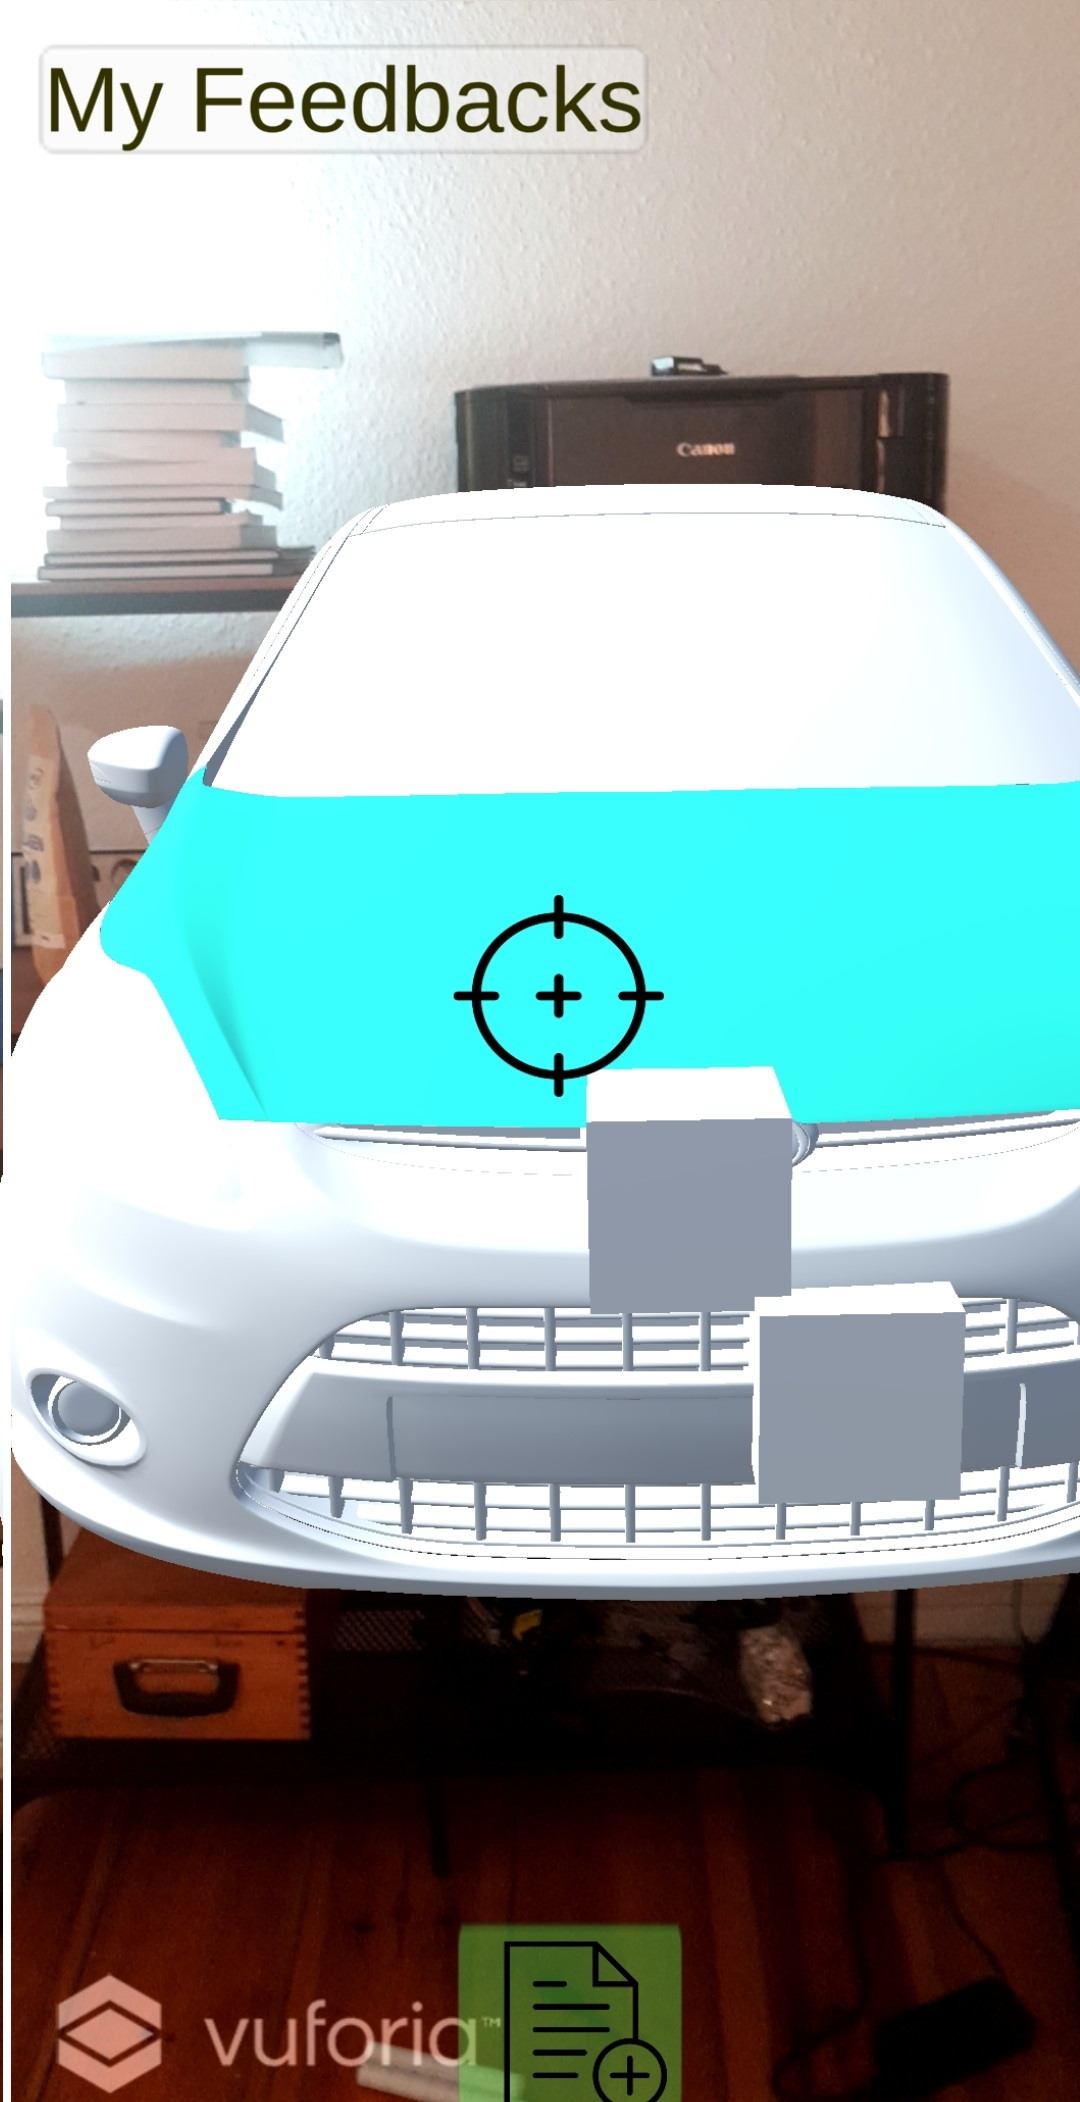
\includegraphics[width=.65\linewidth]{resources/implementation/crossfade_create.jpg}
		\captionof{figure}{Digitaler Protottyp \\ Crossfade Methode Erstellen\\Quelle: Eigene Darstellung}
		\label{fig:crossfade_create}
	\end{minipage}%
	\begin{minipage}{.4\textwidth}
		\centering
		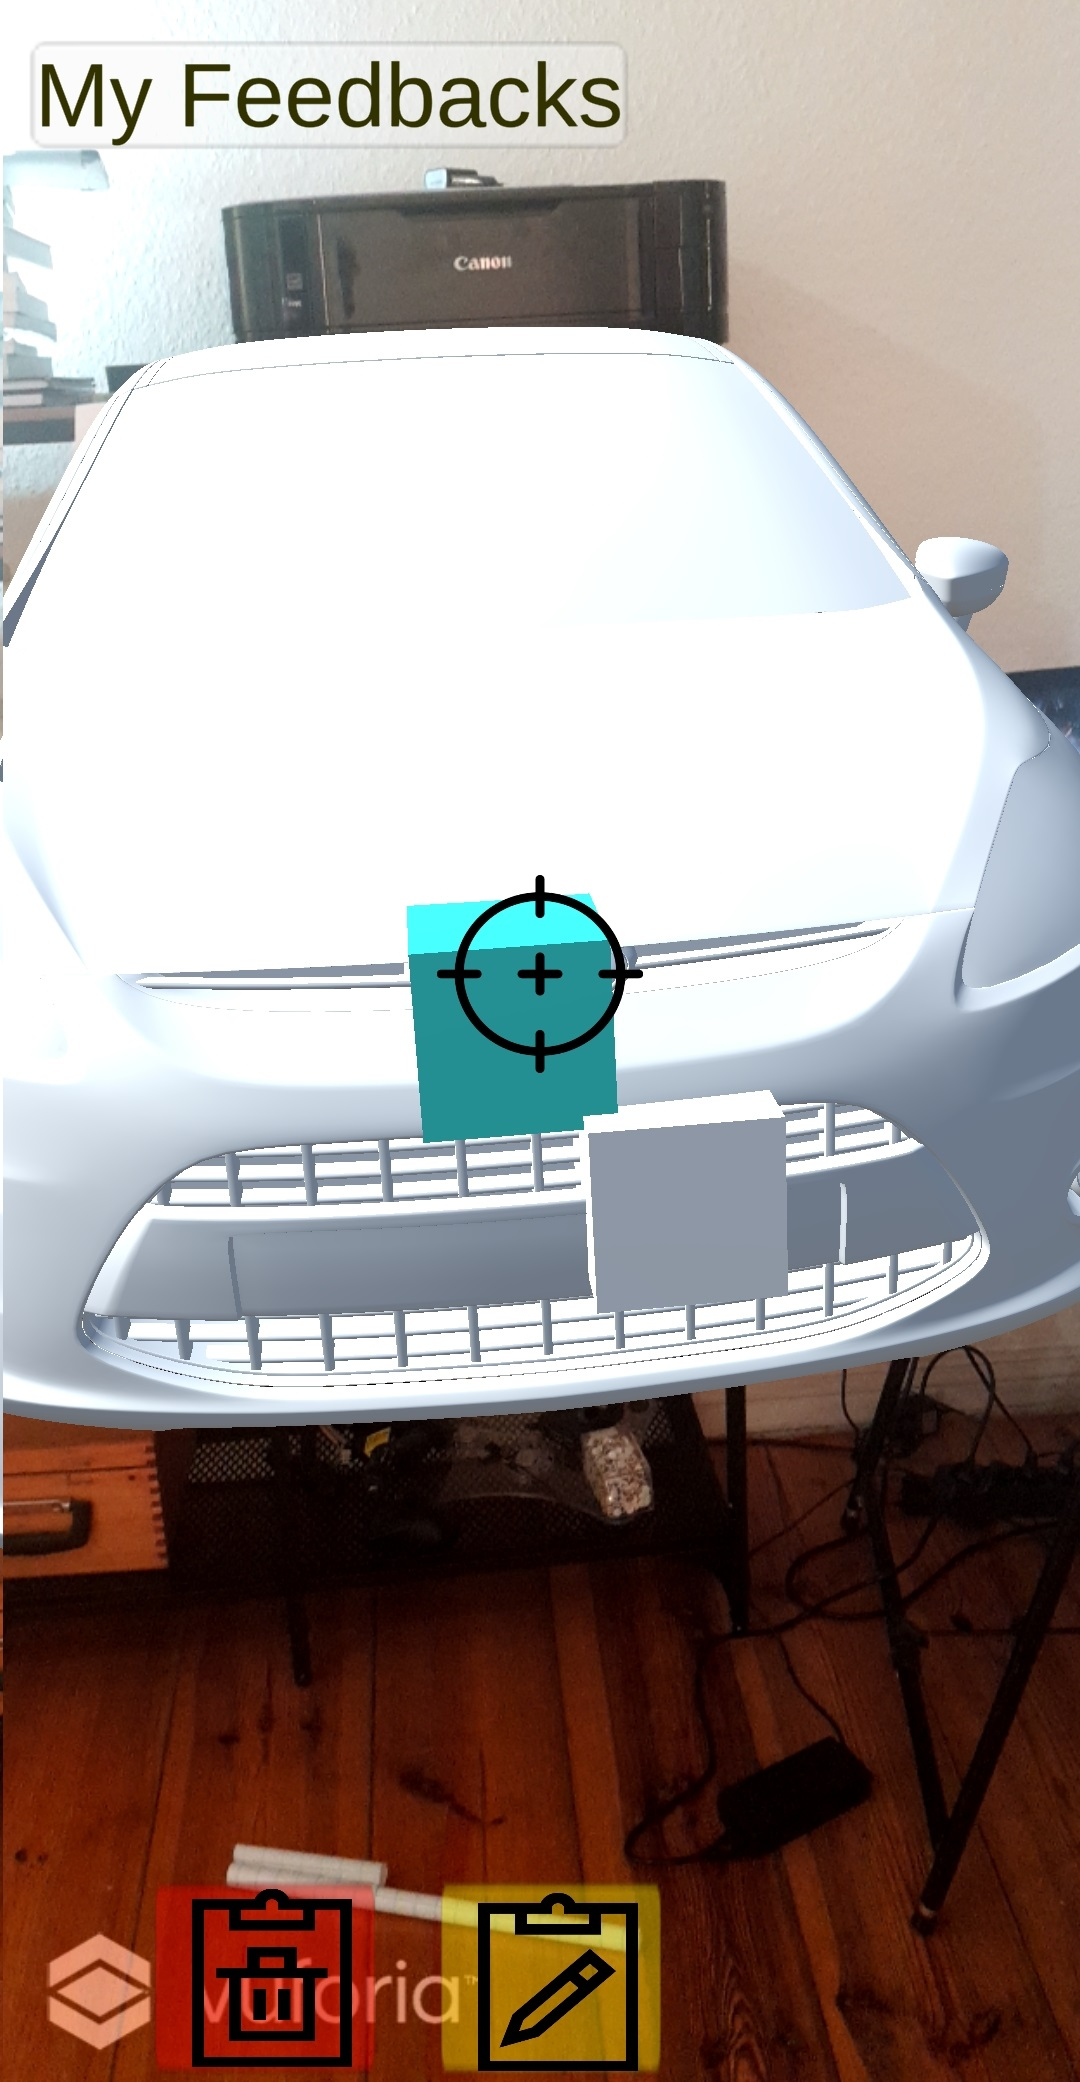
\includegraphics[width=.65\linewidth]{resources/implementation/crossfade_edit.jpg}
		\captionof{figure}{Digitaler Protottyp \\ Crossfade Methode Bearbeiten/ Löschen\\Quelle: Eigene Darstellung}
		\label{fig:crossfade_edit_delete}
	\end{minipage}
\end{figure}

Diese Methode wurde von vier Testnutzern getestet und als zu umständlich empfunden worden. Was bei der Nutzung aller Testnutzer beobachtet werden konnte, dass diese intuitiv auf eine beliebige Stelle oder auf den Fadenkreuz auf dem Bildschirm 
getippt haben und sehr spät gemerkt haben das sich am unteren Rand des Bildschirm ein Button zum Anlegen befindet. Die Anmerkungen der Nutzer zu dieser Variante waren, dass sie intuitiv angenommen haben dass sie auf das Bildschirm klicken oder wischen 
müssten um eine Stelle auf dem Produkt auszuwählen. Dies könnte sich dadurch erklären dass eine gewisse Erwartungskonformität durch die Nutzung von Touchscreen Oberflächen vorhanden ist. Zudem gab es die Anmerkung dass es recht Umständlich sei die Stelle 
am Produkt anvisiert zu lassen und gleichzeitig die Aufmerksamkeit auf das Button zum auswählen zu richten. Das zittern der Hände würde diesen Umstand weiter verschlimmern. 

So wurde entschieden mit der Implementierung der \textit{Relativ Pointing} Methode für das Zeigen und Auswählen auf dem Produkt fortzufahren.  Die Informationsverarbeitung während der Nutzung der Touchscreen Oberfläche für das Zeigen und Auswählen einer 
Stelle oder eines bereits existierenden Feedback veranschaulicht das Flussdiagramm auf Abbildung \ref{img:flow}. 

Die Interaktion mit der \textit{Relativ Pointing} Methode wurde wie folgt umgesetzt. 

Während des gesamten Vorangs wird ein Ray-Cast durchgeführt. Die Interaktion ist in drei Phasen aufgeteilt, die Phase in welcher der Finger auf das Bildschirm angelegt wird, die Phase in welcher der Finger auf dem Touch Bildschirm bewegt wird und die Phase in dem 
der Finger angehoben wird. Es wird ein Strahl ausgehend vom Position des Fingers auf dem Bildschirm, in die Welt hinein gesendet. 

Folgend sind die Interaktion Schritte beschrieben:

\begin{enumerate}
	\item Der Nutzer legt sein Finger auf das Touchscreen an. Dies ist der Startposition für das Zeigen. 
	\begin{enumerate}
	\item Es wird zunächst überprüft ob der Strahl ein bereits vorhandenes Feedback getroffen hat. Ist dies der Fall wird auf die aktuelle Position des Fingers ein zwei Buttons zum Editieren oder Löschen des Feedback platziert. Diese Buttons bleiben für eine bestimmte Zeit eingeblendet (z. B. 4 Sekunden) und werden ausgeblendet entweder wenn die Zeit abgelaufen ist oder wenn der Finger erneut an das Bildschirm an eine andere Stelle angelegt wird. 
	\item Falls der Finger einen Bereich auf dem Produkt trifft, werden alle auf dem Produkt vorhandenen Feedback ausgeblendet damit während des Auswahlvorgangs keine Bereiche auf dem Produkt verdeckt werden. Der Zeiger welches durch eine rote Kugel repräsentiert wird, wird an der Stelle die der Strahl auf dem Produkt getroffen hat platziert.
	\end{enumerate} 
	\item Der Nutzer bewegt sein Finger auf dem Touch Bildschirm.
	\begin{enumerate}
		\item Es wird überprüft ob ein Produktteil bereits Blau eingefärbt und so in Fokus gerückt ist. Ist dies der Fall, wird das eingefärbter Teil in die Standardfarbe gefärbt sodass dieser nicht mehr hervorgehoben wird und das Teil welches vom ausgesendeten Strahl getroffen wird wird in Blau eingefärbt.
		\item Ist auf dem Produkt ein Teil bereits in den Fokus gerückt. Wird das Teil welches vom Strahl getroffen wird Blau eingefärbt.  
		\item Der Zeiger wird auf dem Produkt in jeder Frame in welcher der Finger in Bewegung ist auf die Stelle auf dem Produkt gesetzt die der ausgesendete Strahl trifft.
	\end{enumerate} 
	\item Der Nutzer hebt sein Finger vom Bildschirm ab. Es werden alle vorhanden Feedback wieder auf dem Produkt eingeblendet. Es wir ein Button zum auswählen der Stelle auf dem sich aktuell der Zeiger auf dem Produkt befindet auf der Stelle auf dem der Finger des Nutzers beim anheben des Fingers auf dem Bildschirm befand eingeblendet.
\end{enumerate} 

Diese Methode wurde ebenfalls von Test Nutzern (darunter auch eine Nutzerin welche die \textit{Crossfade} Methode nicht getestet hatte) getestet und Iterationsschritte schnell verstanden. 

\begin{figure}[H]
	\centering
	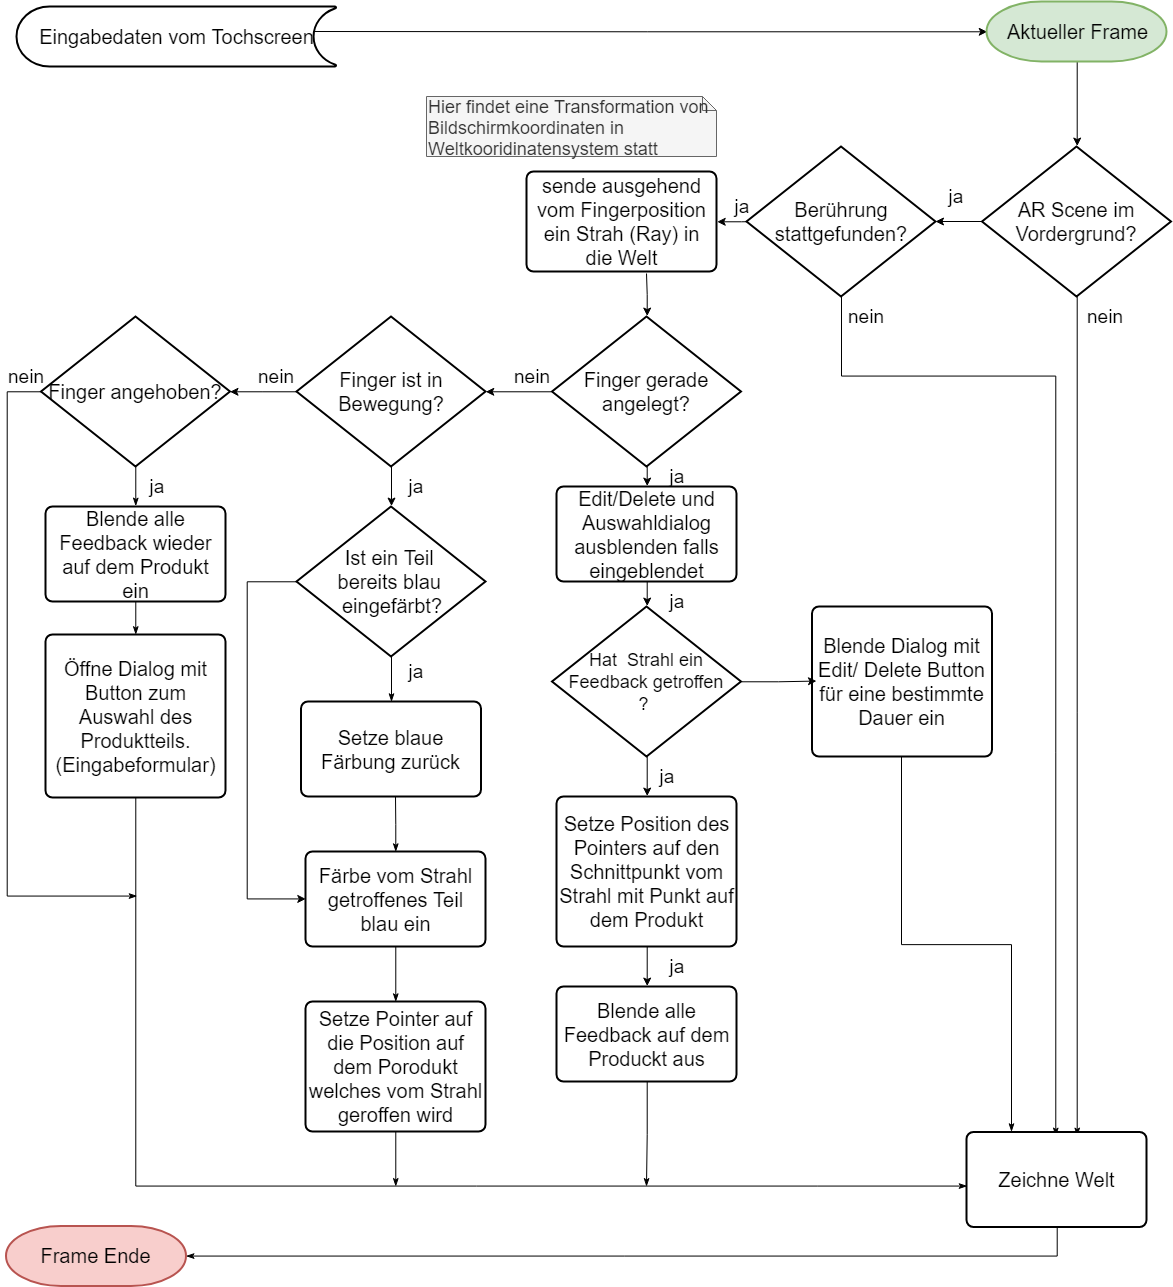
\includegraphics[width=1.0\textwidth]{resources/implementation/flussdiagram_selection.png}
	\caption{Flussdiagramm - Verarbeitung des Touchscreen Berührvorgang \\Quelle: Eigene Darstellung}
	\label{img:flow}
\end{figure}

\section{Vorstellung des digitalen Prototypen}

Im Folgenden wird der digitale Prototyp vorgestellt. 

Die Überlagerung der realen Produkte konnte mit verwendeter Tracking Methode leider nicht optimal erreicht werden. Zum einen die Skalierung der virtuellen Objekte welche relativ zur 
Größe des Image Targets Skaliert wurden konnte nicht passgenau bestimmt werden. Zum anderen musste das Image Target so auf dem Produkt ausgerichtet werden das das virtuelle Modell das 
physische passgenau überlagert. Das Ergebnis der Überlagerung ist auf Abbildung \ref{fig:ueberlagerung} zu sehen. Trotz dessen konnte jedoch mit der eingesetzten Interaktionstechnik 
eine Stelle am Produkt ausgewählt und Feedback angelegt werden. Der Bezug zu der Stelle am realen Produkt konnte trotz schlechter Überlagerung hergestellt werden. 

Auf Abbildung \ref{fig:createdigi} ist eine Ansicht zu sehen in welcher der Nutzer eine Stelle für die Erstellung eines Feedback ausgewählt hat. Wird auf das grüne Button geklickt, gelangt man 
in die auf Abbildung \ref{fig:secondform} dargestellte Formularansicht. 

\begin{figure}[H]
	\label{tab:example}
	\centering
	\begin{minipage}{.45\textwidth}
		\centering
		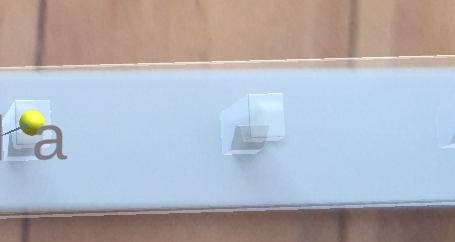
\includegraphics[width=.85\textwidth]{resources/implementation/ueberlagerung.png}
		\captionof{figure}{Digitaler Protottyp \\ Überlagerung des realen Produktes. Nicht optimal. \\Quelle: Eigene Darstellung}
		\label{fig:ueberlagerung}
	\end{minipage}%
	\begin{minipage}{.45\textwidth}
		\centering
		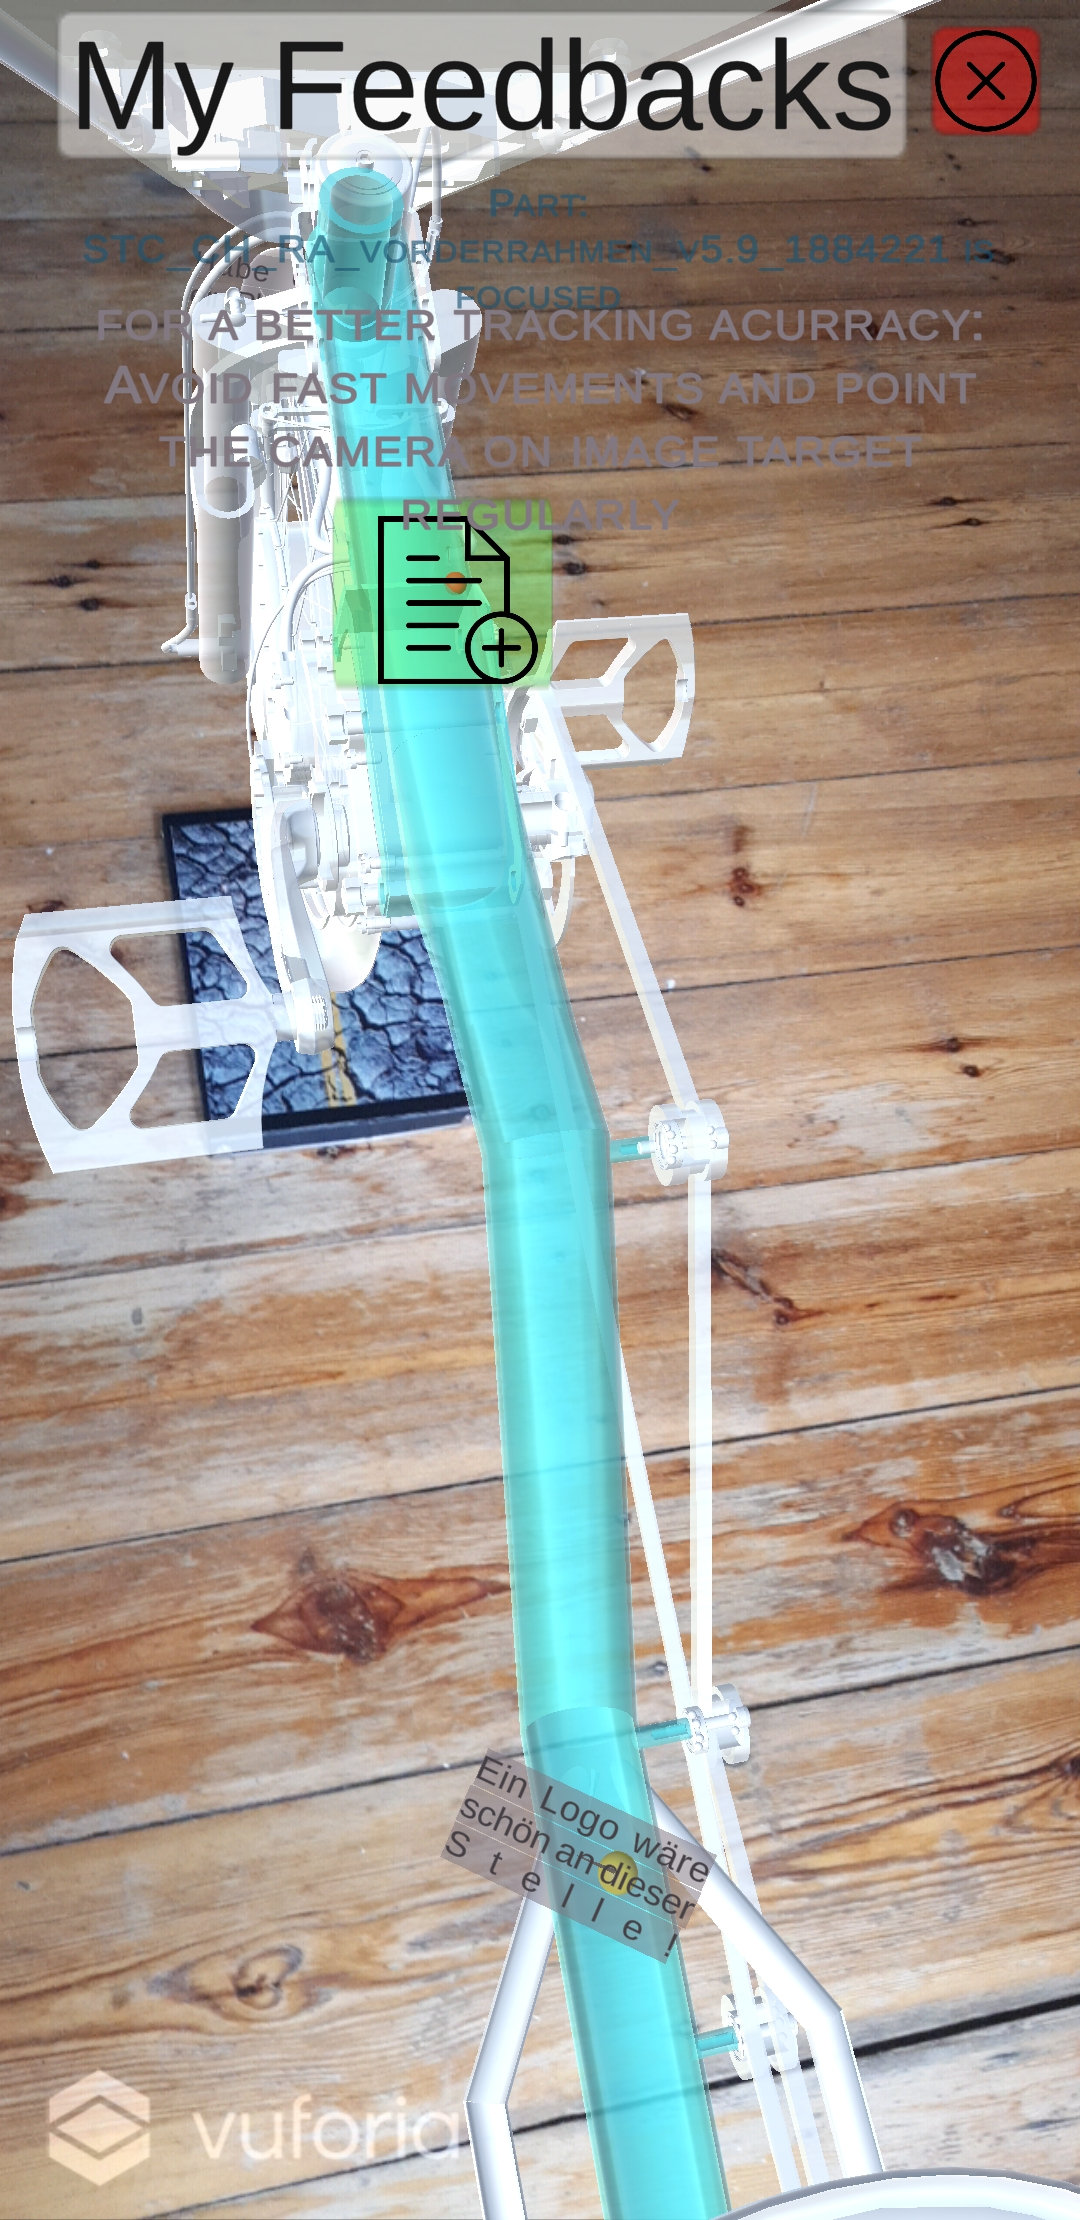
\includegraphics[width=.95\linewidth]{resources/implementation/annocreate.jpg}
		\captionof{figure}{Digitaler Protottyp \\ Auswahl einer Stelle am Produkt. \\Quelle: Eigene Darstellung}
		\label{fig:createdigi}
	\end{minipage}
\end{figure}

Für die Bearbeitung und Löschung von Feedback gibt es mit zwei unterschiedliche Darstellungsformen aus die, diese Aktionen durchgeführt werden können. 
Die Annotationsansicht welche auf Abbildung \ref{fig:annotationview} dargestellt ist sowie die Listenansicht welches auf Abbildung \ref{fig:listview} zu sehen ist. 

\begin{figure}[H]
	\label{tab:example}
	\centering
	\begin{minipage}{.45\textwidth}
		\centering
		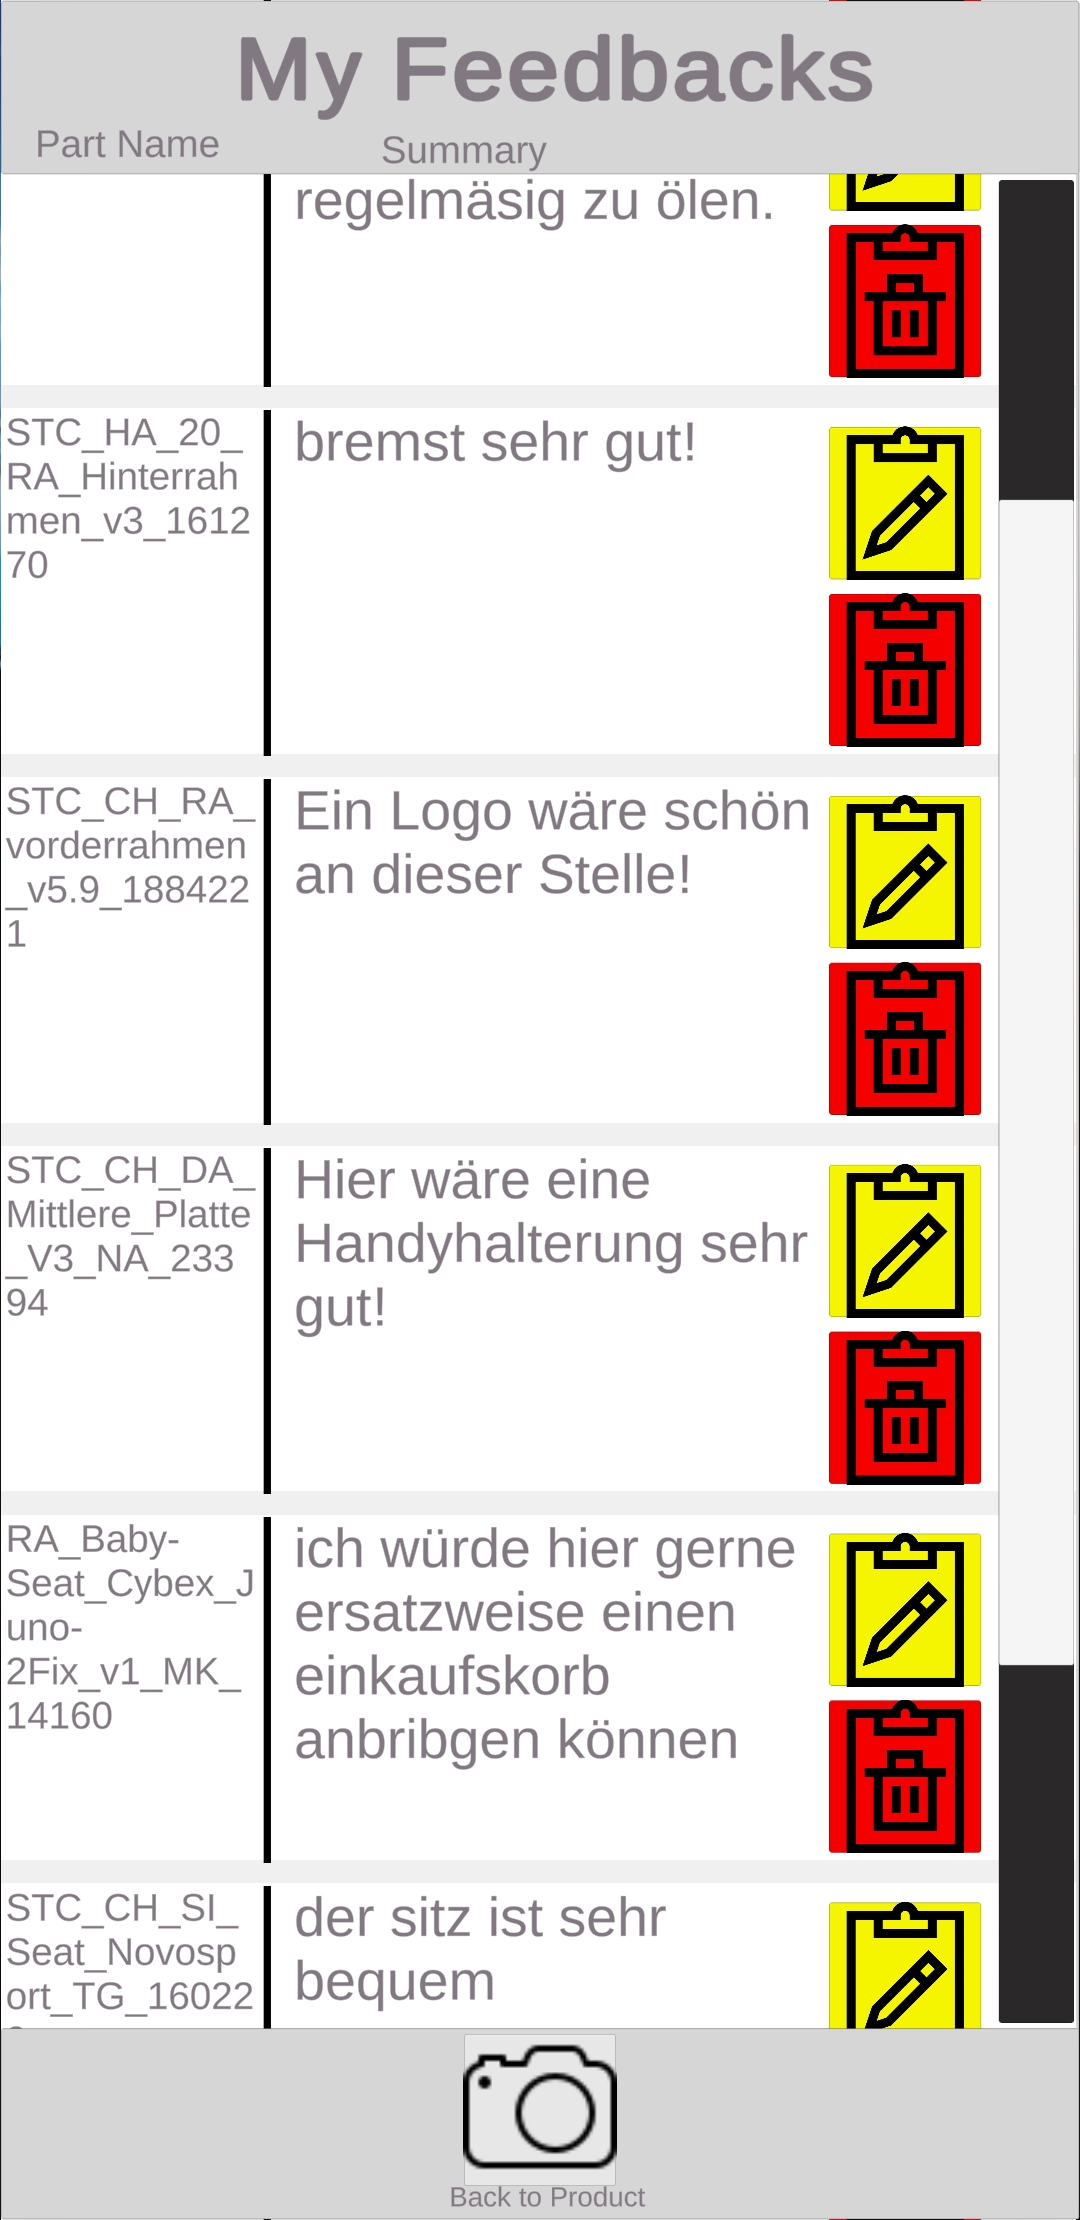
\includegraphics[width=.95\linewidth]{resources/implementation/listview.jpg}
		\captionof{figure}{Digitaler Protottyp \\Listenansicht \\Quelle: Eigene Darstellung}
		\label{fig:listview}
	\end{minipage}%
	\begin{minipage}{.45\textwidth}
		\centering
		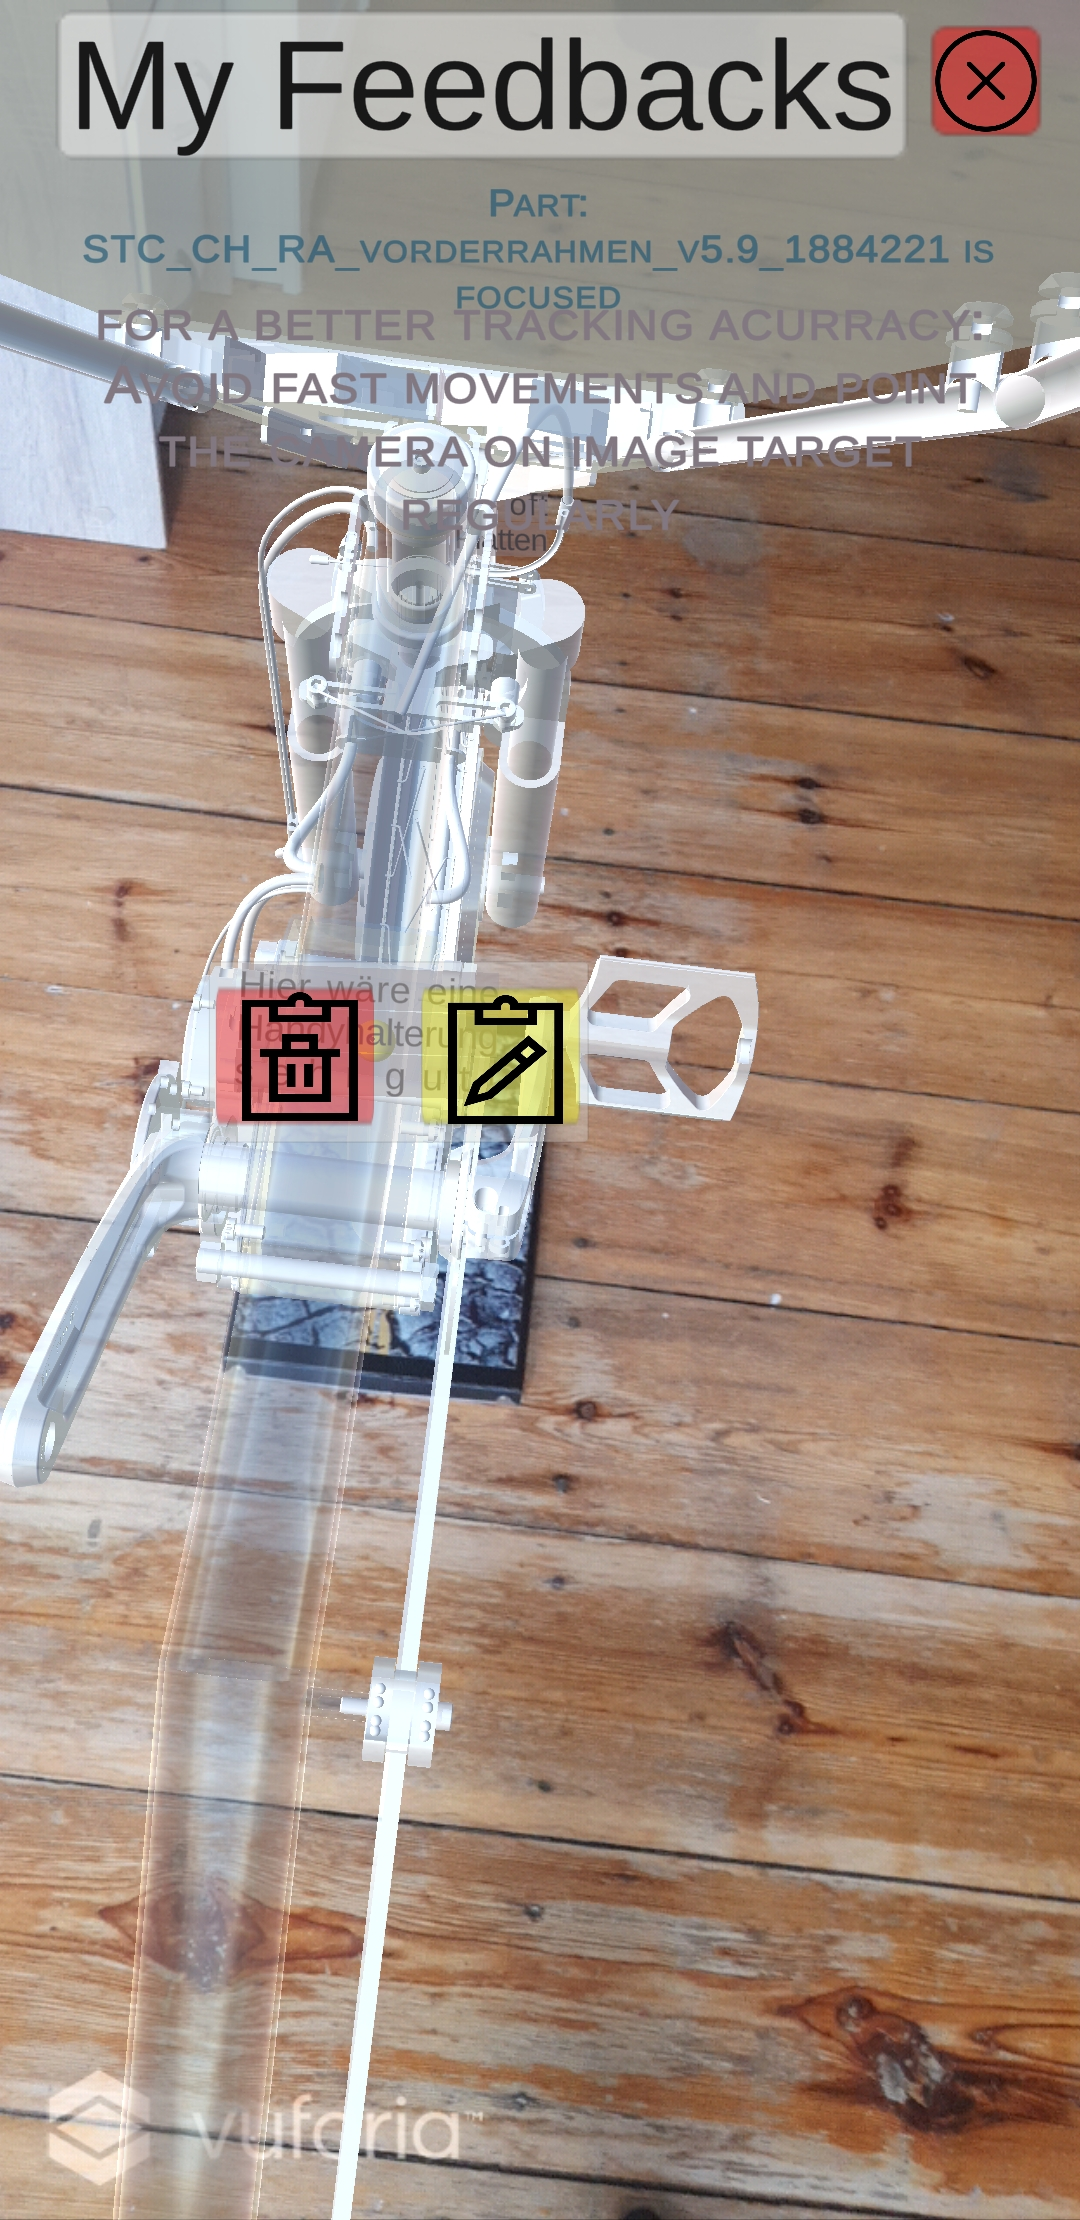
\includegraphics[width=.95\linewidth]{resources/implementation/annotationview.jpg}
		\captionof{figure}{Digitaler Protottyp \\ Annotationsansicht \\Quelle: Eigene Darstellung}
		\label{fig:annotationview}
	\end{minipage}
\end{figure}

Auf Abbildung \ref{fig:firstform} ist eine erste Version des Formular Ansicht für das Anlegen eines neuen Feedback zu sehen. 
Viele Elemente dieser Ansicht wurde von den Test Nutzern nicht verstanden. Insbesondere war ging nicht klar hervor wofür die einzelnen Kategorien 
stehen sowie was die Felder \textit{Impact} und \textit{Request Support} bewirken. Außerdem wurde festgestellt dass, das Formular keine Möglichkeit 
zur näheren Spezifizierung, ob auf die ausgewählte Stelle am Produkt oder das Produktteil Bezug genommen wird ermöglicht. 

So das Formular überarbeitet. Die überarbeitete Version ist auf Abbildung \ref{fig:secondform} zu sehen. Zu den Feldern welche nicht gut verstanden wurden,
wurden Beschreibungen hinzugefügt, welche diese näher beschreiben. Zudem wurden Icons verwendet welche die Bedeutung der Elemente verbildlichen. An einigen Stellen 
wurden Gestaltungsgesetze angewendet. Zum Beispiel wurde das  Gesetzt der Nähe verwendet und ähnliche Kategorien wie Design und New Usecase sowie Frage und Anleitung näher beieinander dargestellt. 
Des weiteren wurden die Buttons zum "Reset" zum Zurücksetzten der Eingaben sowie das Button zum zurückkehren in die AR Ansicht mit einem Abstand zum "Submit" Button, für die Bestätigung der Eingaben 
dargesetllt. Das Gesetzt der Unentschlossenheit wurde angewendet um zu zeigen dass die zwei Kontrollkästchen für die Auswahl ob Bezug auf eine bestimmte Stelle am Produkt genommen wir oder auf ein 
Produktteil zusammen gehören. 

\begin{figure}[H]
	\label{tab:example}
	\centering
	\begin{minipage}{.45\textwidth}
		\centering
		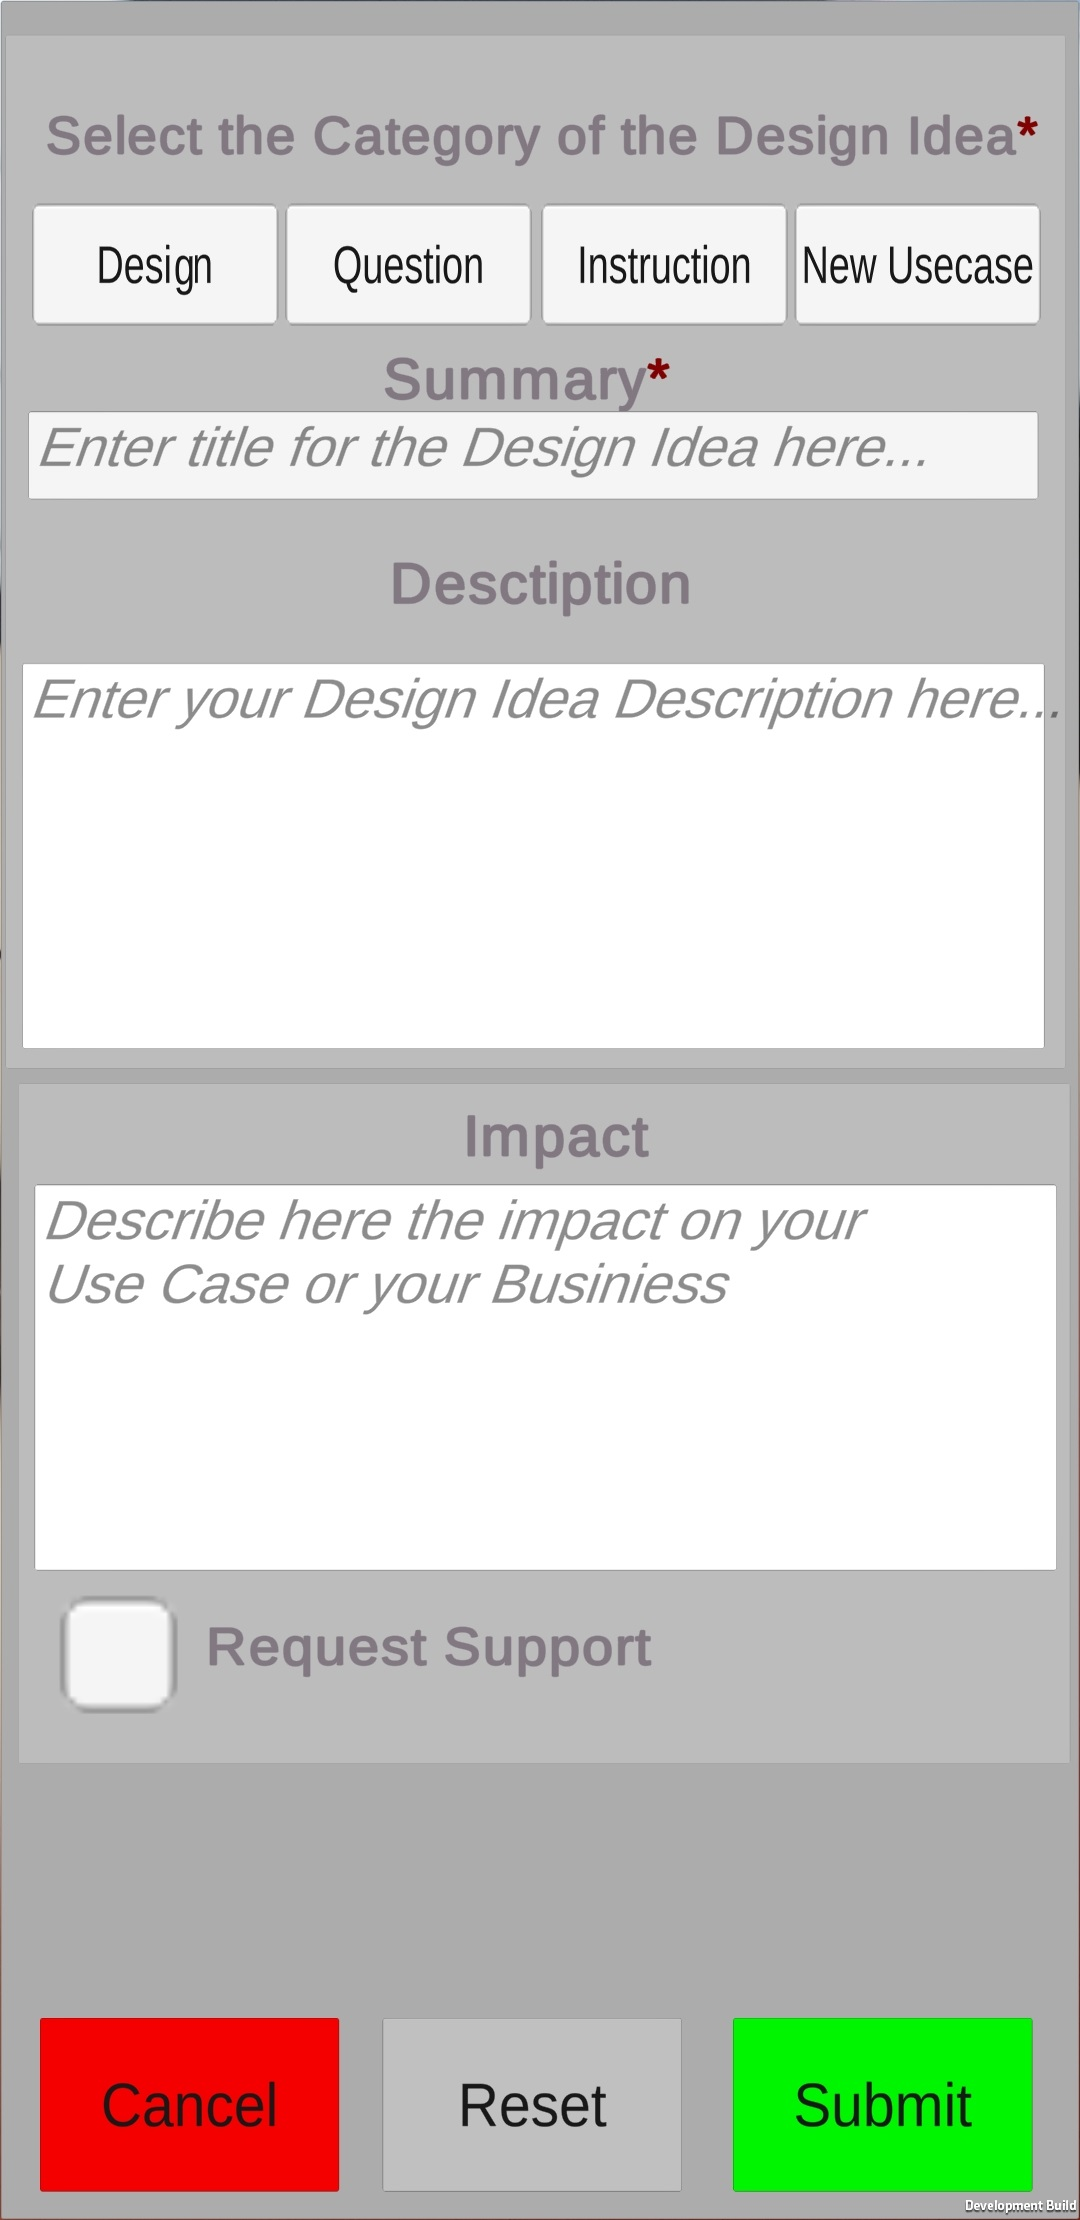
\includegraphics[width=.95\linewidth]{resources/implementation/firstform.jpg}
		\captionof{figure}{Digitaler Protottyp \\Formualransicht Version 1\\Quelle: Eigene Darstellung}
		\label{fig:firstform}
	\end{minipage}%
	\begin{minipage}{.45\textwidth}
		\centering
		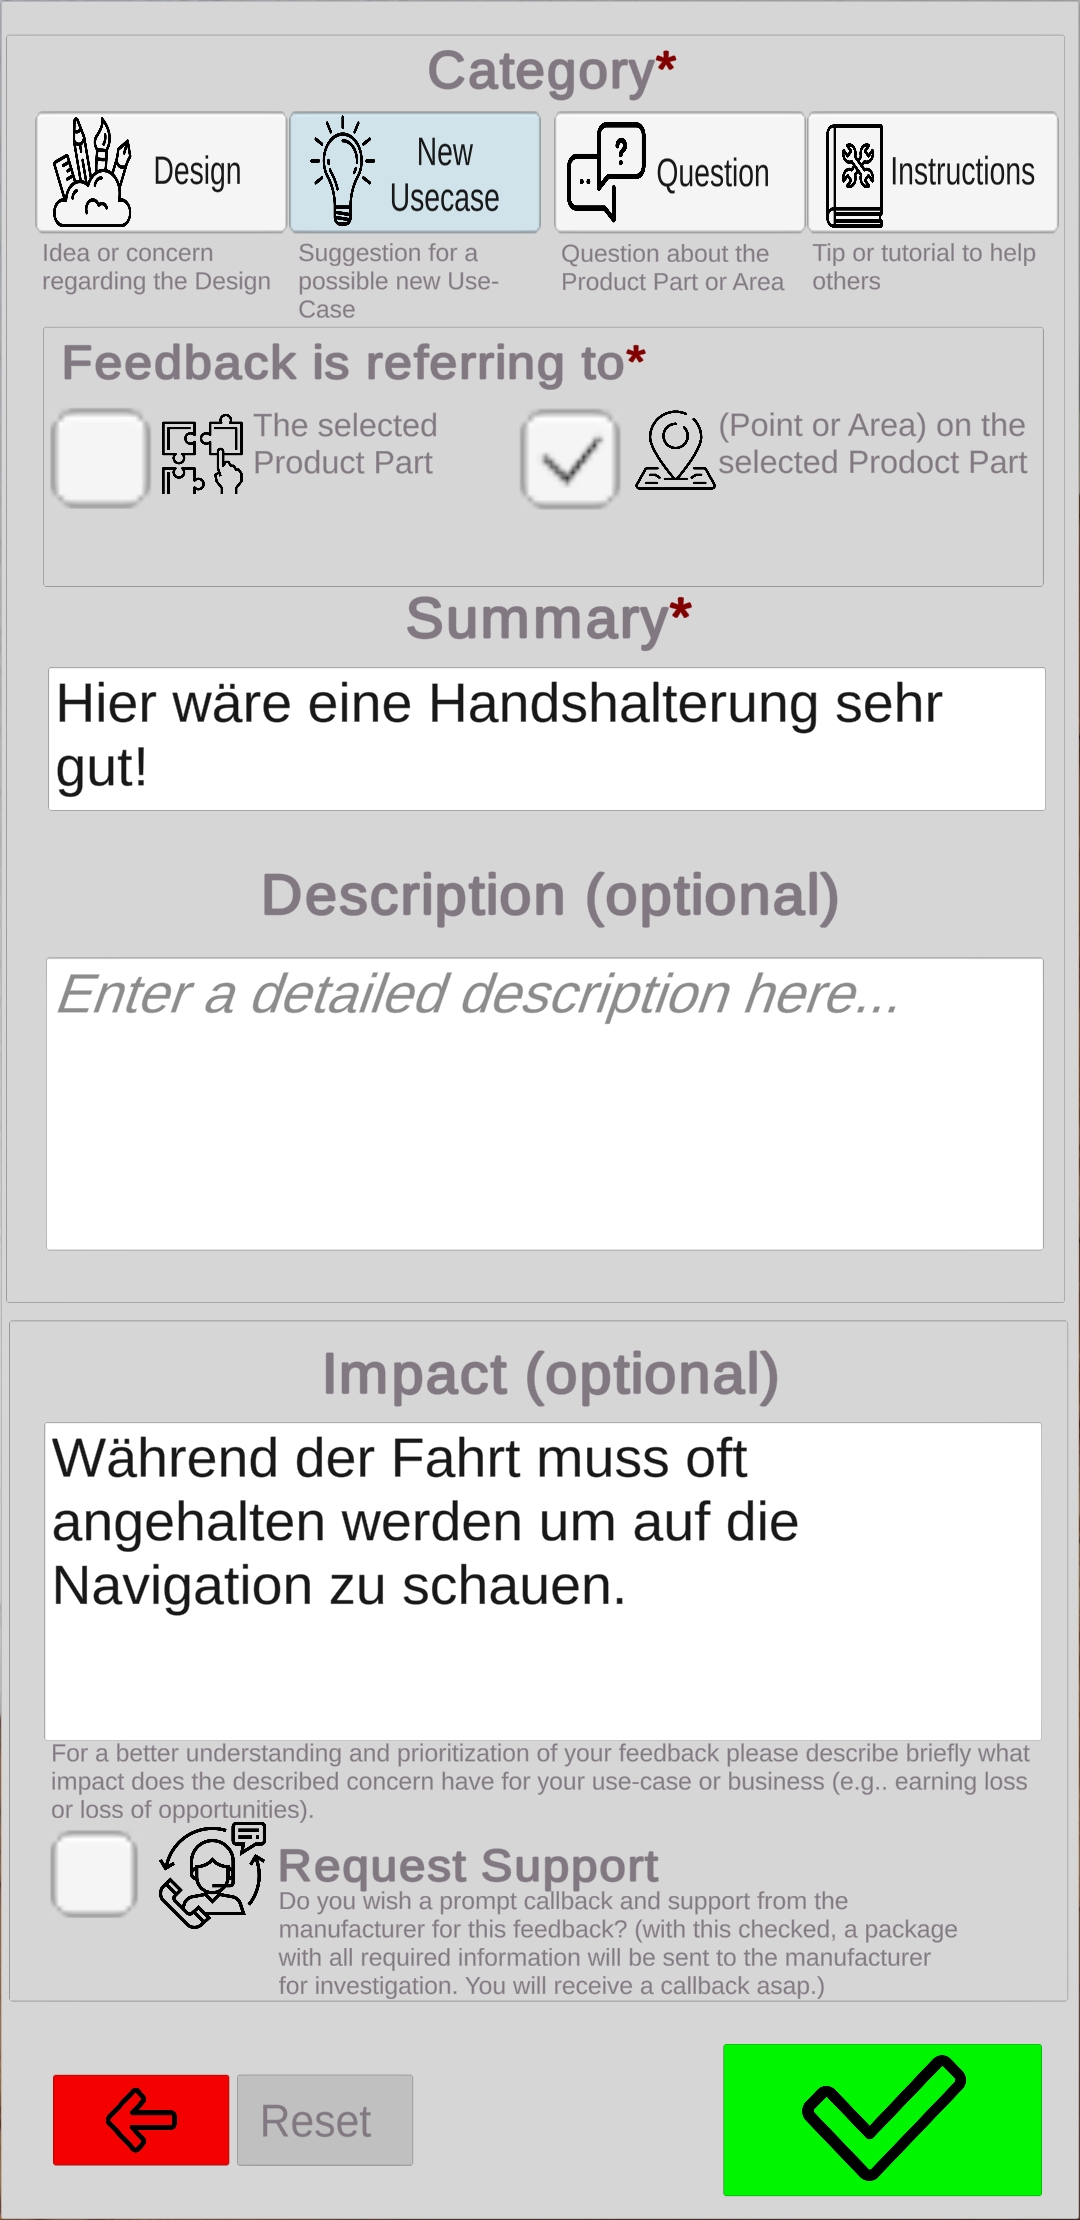
\includegraphics[width=.95\linewidth]{resources/implementation/secondform.jpg}
		\captionof{figure}{Digitaler Protottyp \\ Formularansicht Version 2\\Quelle: Eigene Darstellung}
		\label{fig:secondform}
	\end{minipage}
\end{figure}

\section{Zeiterfassung für die Studie}

Für die Zeiterfassung der durchzuführenden Aktionen in der Studie wurde beschlossen für jede durchgeführte Aktion
jeweils in der Start Methode der SelektionManager Klasse die Zeitmessung zu starten und bei der jeweiligen Aktion zu stoppen.
Die Start Methode wird wird nur einmal im Lebenszyklus des Skriptes ausgeführt und wird vor der ersten Ausführung der Update Funktion ausgeführt welcher in jeder Frame ausgeführt wird. \cite{Unity}

Für die Erstellung und Bearbeitung wurde die Zeit jeweils in der Methode gestoppt in welcher die Szene für die Formular Ansicht \ref{fig:secondform}
geöffnet wurde. Für das Löschen wurde die Zeit in der Methode gestoppt in welcher die Lösch-Methode des StorageManagers aufgerufen wurde. 

Der Datentyp (Sihe Abbildung \ref{img:entitytype}) für ein Feedback wurde um drei weitere Felder ergänzt in welcher die Zeiten für die jeweiligen Aktionen festgehalten wurden. In drei neuen Felder vom Datentyp Integer wurde jeweils die Zeit
in Millisekunden gespeichert die benötigt wurde um in das Formular zum Erstellen bzw. zum Bearbeiten zu gelangen sowie die Zeit die die benötigt wurde um ein Feedback zu löschen. 
Die Werde wurden in eine XML Datei gespeichert wenn die Applikation beendet wurde. 

Es wurde vorausgesetzt dass nach jeder Aufgabe die Anwendung neugestartet werden musste damit die Startzeit, da diese in der Start Methode des SelektionManager Klasse beginnt für die neue Aufgabe zurückgesetzt wird. 
Sicherlich hätte dies eleganter gelöst werden können, doch diese Methode wurde getestet und als sicher empfunden. Auf Grund des Zeitmangels wurde die Zeitmessung bei dieser Methode belassen.
 \clearpage
\chapter{Nutzerstudie}

\section{Planung der Nutzerstudie}

\subsection{Studiendesign}

\subsection{Prozedur}

\section{Durchführung}

\subsection{Erheben der Evaluationsdaten}

\subsection{Ergebnisse}

\begin{figure}[H]
	\centering
	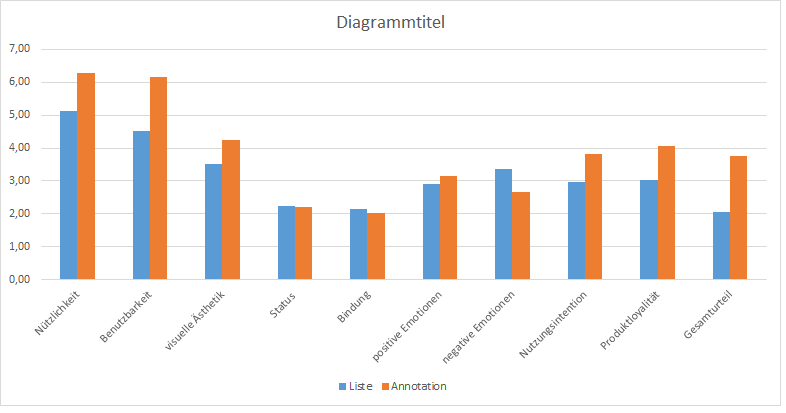
\includegraphics[width=1.0\textwidth]{resources/evaluation/diagrammittel_vergleich_liste_annotation.png}
	\caption{Vergleich der Mittelwerte aus meQue Fragebogen für Listen/Annotation Ansicht \\Quelle: Eigene Darstellung}
	\label{img:avg_meQue_listAnnotation}
\end{figure}

\section{Folgerung}

\section{Fazit der Nutzerstudie} \clearpage
\chapter{Fazit}

Dieses Kapitel fasst die Arbeit zusammen. Es wird mit Rückblick auf die Zielsetzung sowohl Erreichtes reflektiert als auch Herausforderungen die sich während der Arbeit gestellt haben und mögliche Verbesserungen hervorgehoben. Abschließend werden in einem Ausblick Erweiterungsmöglichkeiten beschrieben. 

\section{Zusammenfassung}

Im Kapitel \ref{anlayse_capter} dieser Arbeit wurden Forschungen im Gebiet der Informationsdarstellung in virtuellen Umgebungen (Abschnitt \ref{brand_abschnitt}) sowie Methoden für das 
Zeigen und Auswählen in AR-Anwendungen (Abschnitt \ref{pointer_section}) betrachtet. Im Abschnitt \ref{ipi_section} wurden Arbeiten betrachtet, welche ein Konzept für das in dieser Arbeit entworfene System vorstellen
und unterschiedliche Umsetzungsmöglichkeiten beschreiben. 

Im Kapitel \ref{conception_chapter} wurden im Rahmen eines Workshops anknüpfend an die im Kapitel \ref{CapterFundamentals} Abschnitt \ref{UsaEng} beschriebene Methode des Usability Engineering, Nutzerprofile erstellt, die Aufgaben 
der Nutzer analysiert und Anforderungen für den Prototypen definiert. Darauf aufbauend wurde im Abschnitt \ref{lowfi} ein Papierprototyp erstellt. Dieser wurde einerseits genutzt um die Abdeckung der definierten Anforderungen 
zu überprüfen, andererseits auch als grobe Vorlage für die Entwicklung des digitalen Prototypen im Kapitel \ref{implementation}. Zusätzlich zum Papierprototypen wurde als Grundlage für die Implementierung im Abschnitt \ref{objentwurf} ein Datentyp für ein Feedback definiert sowie ein Klassendiagramm erstellt. 

Im Kapitel \ref{implementation} wurden zunächst verschiedene zwei verschiedene Tracking Frameworks und unterschiedliche Tracking Methoden ausprobiert. 
Nachdem das Tracking mit Verwendung eines 3D-Modell des physischen Produktes nicht funktioniert hat, wurde beschlossen ein Image Target für das Tracking mit Nutzung
des Vuforia Frameworks zu verwenden. 
Es wurden zwei im Kapitel \ref{anlayse_capter} behandelte Methoden für das Zeigen und Auswählen implementiert, diese wurden von Testnutzern getestet wurde die hinsichtlich ihrer Usability besser geeignete Methode in den Prototypen aufgenommen. Abschließend wurde im Kapitel \ref{implementation} ein Eingabeformular
gestaltet, welches mit Berücksichtigung der im Kapitel \ref{conception_chapter} identifizierten Anforderungen die Erstellung eines Feedback ermöglicht.  

Wie in der Zielsetzung vorgenommen, wurde im Kapitel \ref{study} der im Kapitel zuvor implementierte Prototyp hinsichtlich seiner Usability für die Aktionen: Erstellung, Bearbeitung und Löschung eines
Feedback evaluiert. Dabei hat sich ergeben, dass der entwickelte Prototyp für die Bearbeitung dieser Aufgaben eine hohe Usability aufweist, jedoch in Eigenschaften, welche in der Produktwahrnehmen eher 
in den Bereich des Nutzungserlebens (engl. User Experience, kurz UX) zugeordnet werden deutliches Verbesserungspotenzial aufweist. 

Zudem wurden in diesem Kapitel für die Bearbeitung von Feedback, zwei unterschiedliche Darstellungsformen verglichen und festgestellt wurde, dass 
die Darstellung der Feedbacks als Annotationen auf den Produkten im Vergleich zu einer Listenansicht zu mehr Zufriedenheit bei der Bearbeitung der Aufgabe führt uns sich daher besser eignet. 

Abschließend werden in diesem Kapitel die Arbeit hinsichtlich aufgetretenen Herausforderungen, mögliche Verbesserungen erläutert sowie in einem Ausblick Erweiterungsmöglichkeiten vorgestellt.  

\section{Kritischer Rückblick}

Reflektierend betrachtend kann hinsichtlich der Zielsetzung dieser Arbeit gesagt werden, dass diese mit der durchgeführten Nutzerstudie erreicht wurden.
Jedoch gab es einige Schwächen in der Umsetzung, welche in zukünftigen Arbeiten verbessert werden können. 

Zu diesen zählen organisatorische Schwächen, die sich auf folgende Punkte ausgewirkt haben:  

\begin{itemize}
\item{Für die Erarbeitung einer besser geeigneteren Lösung für die Überlagerung des physischen Produktes wurde nicht ausreichend Zeit eingeplant, sodass auf eine Lösung zurückgegriffen werden musste bei der 
die Überlagerung nicht optimal funktionierte.} 

\item{Das physische Produkt konnte für die Nutzerstudie nicht bereitgestellt werden. Dies hatte zur Folge dass die Darstellung als Annotation ohne eine Überlagerung des physischen Produktes und Listenansicht ohne die Anwesenheit des physischen Produktes getestet werden musste.}
\item{Für die Zeiterfassung für der Aufgabenbearbeitung wurde eine Lösung gewählt, die zwar getestet wurde und als sichere Methode empfunden wurde, jedoch 
keine geschickte Lösung darstellte. Mit dieser Zeiterfassungsmethode musste bei jeder Iteration der Aufgabenbearbeitung die Anwendung neugestartet werden, damit die Zeit für die nächste Aufgabe zurückgesetzt wurde.} 
\end{itemize}


\section{Ausblick}

Der entwickelte Prototyp kann in unterschiedliche Richtungen erweitert werden. Zum Einen können weitere in Kapitel \ref{conception_chapter} Abbildung \ref{img:sysstem_sketch} dargestellten Anforderungen implementiert 
werden. Wie zum Beispiel die Behandlung von Überdeckung, wichtiger Produktteile oder Annotationen. Eine Lösung für das Filtern und die in Clustern zusammenfügen der Annotationen (siehe Beispiel auf Abbildung \ref{img:annotation_clutter}) auf dem Produkt. Es könnte mit Hilfe der auf den Endgeräten verfügbaren Sensoren, dem Feedback weitere Informationen wie zum Beispiel Luftfeuchtigkeit, Helligkeit oder Bilder von den auswählten Stellen hinzugefügt werden. Dies würde die Aussagekraft der Feedbacks mit der Stärke der Darstellungsform Embedded Visualization nämlich (Eigenschaften aus der unmittelbaren Umgebung wahrnehmen zu können) bis zu einem bestimmten Grad stärken. 

Zum Anderen kann der Prototyp wie auf dem von \citeauthor{Kirschner2012} auf Abbildung \ref{img:objekt_centered_ipi} vorgestellten Konzept der objektzentrierten Ansatz der IPI Umsetzung, erweitert werden.
Die Grundlage für den Datenaustausch wurde mit der Erarbeitung eines Datentyps für Feedback und dessen Serialisierung und Deserialisierung erreicht. Im weiteren Schritt können diese Daten zwischen mehreren
Clients ausgetauscht und synchronisiert werden, sodass, wie auf Abbildung \ref{img:objekt_centered_ipi} vorgestellt, ein Informationsausgleich stattfindet und eine asynchrone Kommunikation über das Feedback ermöglicht wird. 

Zudem kann eine Schnittstelle erarbeitet werden mit der Hersteller auf diese Daten in strukturierter und gewichteter Form zugreifen und Erkenntnisse für neue Produktgenerationen gewinnen können.  




 \clearpage

% List of Figures
\listoffigures \clearpage
% List of Tables
\listoftables \clearpage
% Source Code Content
\lstlistoflistings \clearpage

\printindex \clearpage

\printnoidxglossary[title=Glossar] \clearpage

\defbibfilter{scientific}{
	type=article or
	type=inbook or
	type=book or
	type=unpublished or
	type=inproceedings or
	type=incollection or
	type=manual or
	type=phdthesis
}

\printbibliography[heading=bibintoc, filter=scientific, title={Literaturverzeichnis}]\clearpage
\printbibliography[heading=bibintoc, keyword={online}, title={Onlinereferenzen}]\clearpage
\printbibliography[heading=bibintoc, keyword={image}, title={Bildreferenzen}]\clearpage

% Appendix
\appendix
\chapter{}
\addcontentsline{toc}{chapter}{Anhang A}\label{anhangA}

\textbf{Affinitätsdiagramm}:

\begin{figure}[H]
	\centering
	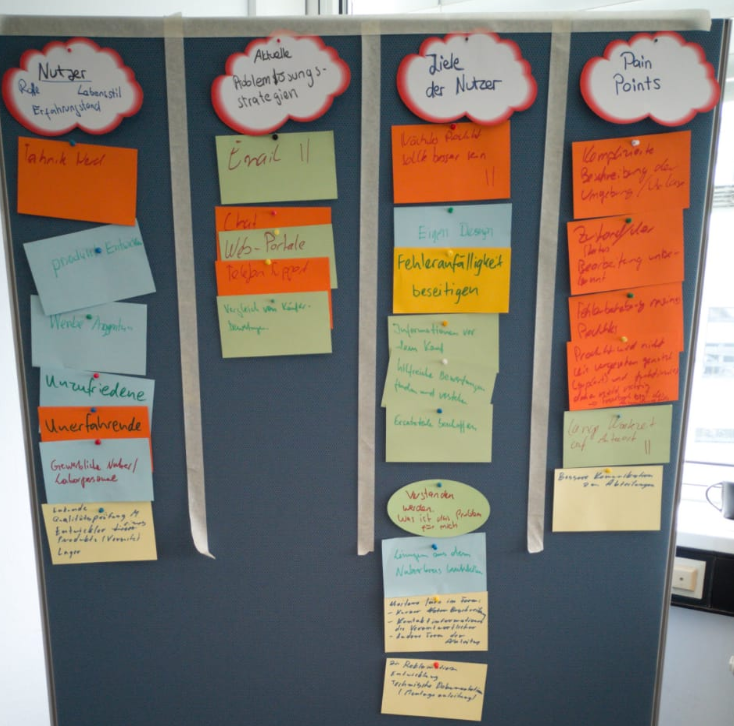
\includegraphics[width=0.50\textwidth]{resources/anhang/Affinitaetsdiagramm.png}
	\caption{Das im Kreativ Workshop am 03.05.2019 entstandene Affinitätsdiagramm welches als Grundlage für die Erstellung von Personas diente. Quelle: Eigene Darstellung}
	\label{img:affinitydiagramm}
\end{figure}

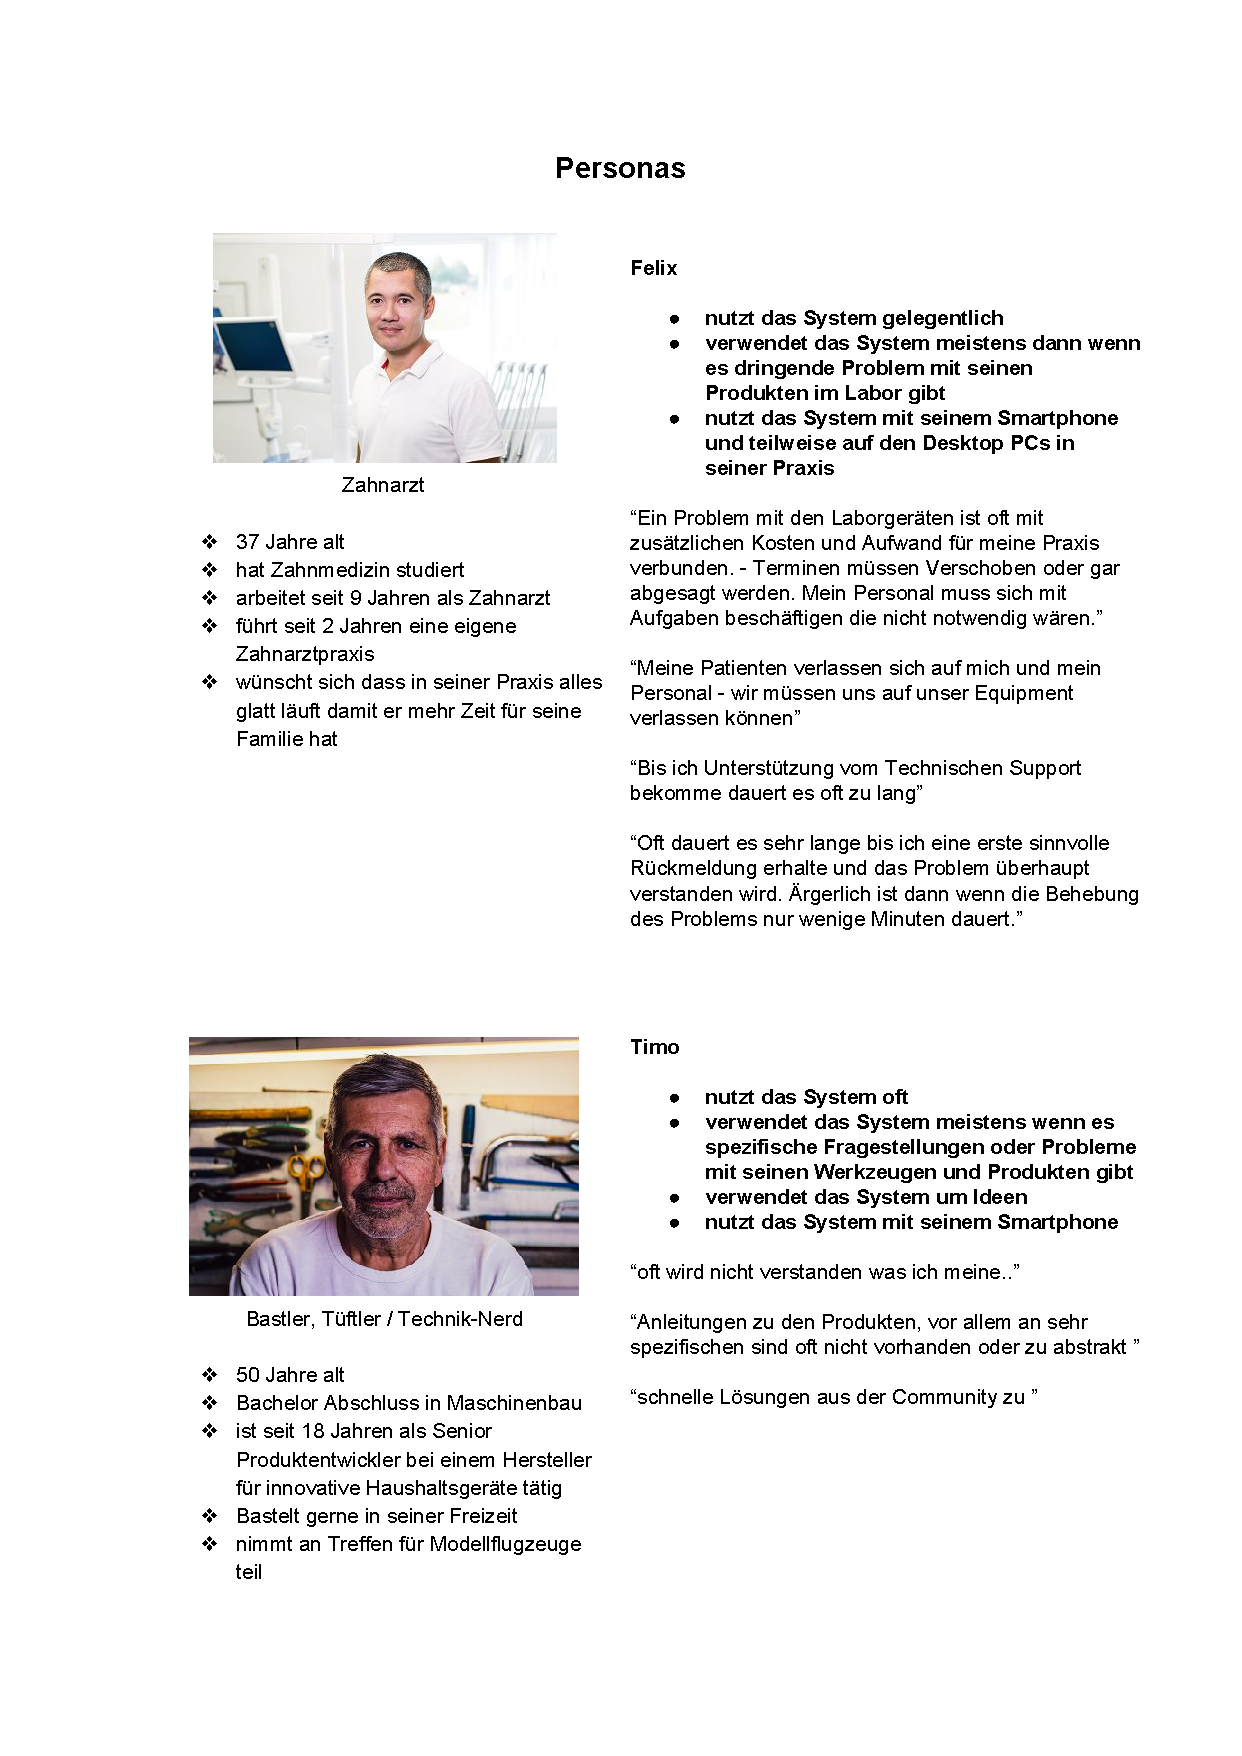
\includepdf[pages=-]{resources/anhang/Personas.pdf}

\addcontentsline{toc}{chapter}{Anhang B}

\textbf{Ist-Szenarien}

\textbf{Felix}

Am Dienstagabend nach der Sprechstunde, entscheidet sich Felix, dem technischen Support des
Herstellers für die Beleuchtungsanlage im Behandlungsraum A, eine E-Mail zu schreiben. Denn die
Leuchte bleibt nicht stabil in seiner Ausrichtung sondern rutscht immer wieder seitlich nach runter.
Nicht nur er ist darüber sehr verärgert sondern auch seine Arzthelferin. Diese muss bei Eingriffen, bei
welchen, Felix eine gute Ausrichtung der Beleuchtung besonders wichtig ist, die Leuchte immer
wieder richtig ausrichten. An manchen Eingriffen ist sie sogar nur noch damit beschäftigt. Er hatte die
Anfrage im Support bereits vor eineinhalb Wochen geöffnet, doch nach der ersten Rückmeldung
folgte nur ein E-Mail Ping-Pong mit Gegenfragen wurden und Vorschläge die er ausprobieren sollte,
jedoch nicht geholfen haben.
Am Mittwochnachmittag erhält Felix eine Antwort. Der Hersteller reagiert diesmal mit dem Angebot
einer Skype-Session. Vier Experten werfen an diesem Videoanruf einen Blick auf die Leuchte und
tauschen sich aus untereinander aus. Einer von diesen wurde, spontan noch dazu gerufen. Nach
kurzer Zeit stellt sich heraus dass an dem Modell welches bei Felix im Praxis in Einsatz ist, ein
Gelenk angebracht ist, welches ein sehr seltenes Exemplar ist. Einem der Support Ingenieure der
dieses Modell zufällig einmal bei einem Kunden im Einsatz gesehen hatte, fällt ein, dass bei diesem
Modell, am Drehgelenk, eines der M6er Schrauben mit einer M7er Schraube ausgetauscht werden
musste, um das Gelenk stabiler zu machen. Der Hersteller schickt daraufhin einen Techniker, und die
Schraube wird ausgetauscht. Felix ist nun besonders verärgert da ein Problem welches in fünf
Minuten behoben werden konnte, ihm und seiner Personal sehr viel Wertvolle Zeit und Mühe gekostet
hat. Die Entschuldigungen des des technischen Supports über den Verlauf dieser Anfrage und die
Beteuerungen diesen Sachverhalt an das Produktmanagement und an das Doku-Team für die
weitere Aufarbeitung weiterzugeben besänftigen seine Verärgerung kaum.

\vspace{2mm}
\textbf{Timo}

Timo freut sich. Es ist endlich Samstag, seine Freundin ist auf Junggesellinnenabschied und er hat
endlich wieder Zeit an seinen Modellfliegern zu werkeln. In drei Wochen findet ein Treffen der
Modellflieger Community am Nachbarort statt und er will seine Flieger bis dahin auf Vordermann
bringen. Vor einigen Wochen hatte er bereits angefangen, sich um das etwas kränklich anhörende
Motor, eines seines seiner Flieger zu kümmern. Vor zwei Wochen hatte er hierzu eine Frage im
Forum “Modellfliegerprofis.de” gepostet und gefragt ob jemand eine Ahnung hätte, ob für die M16er
Schraube links neben der Lötstelle des Einlassventils eine Mutter von einem anderen Hersteller
verwendet werden kann? Ob da schon einmal jemand eine andere Mutter ausprobiert hat und ob dies
geholfen hat.
Er hat wenig Hoffnung dass jemand sinnvoll auf seine Frage antworten konnte, dennoch wirft er mal
einen Blick in das Forum. Wie erwartet haben nur wenige auf seine Frage reagiert und die meisten
haben nicht genau verstanden worum es geht. Er beantwortet noch einige Fragen und schließt etwas
frustriert das Forum.
Drei Wochen später am Treffen der Modellflieger hat er dann die Gelegenheit sein Anliegen den
anderen Technikaffinen direkt am Modell zu zeigen und sich über seine Frage auszutauschen. Es
stellt sich heraus dass, einige den Blog Beitrag gesehen haben, sich jedoch gar nicht erst die Mühe
gemacht haben die betreffende Stelle am Flieger anzuschauen. Vielen geht aus seiner Beschreibung
nicht klar hervor welche Stelle am Flieger er genau meint. Links neben des Einlassventils gebe es
mehrere Lötstellen. Einigen war die Beschreibung zu kompliziert und wussten gar nicht wie eine
M16er Schraube überhaupt aussieht.
Für Timo ist es nicht neu, dass dieser Art von Fragen und Antworten am Ort und Stelle am Modell viel
einfacher beschrieben, diskutiert und oft auch Lösungen gefunden werden können.


\vspace{2mm}
\textbf{Svenja}

Svenja ist fix und alle! Es ist Mittwochabend, sie hat gerade ihr Fitness Workout hinter sich gebracht
und wartet in Ihrem Lieblingskaffee auf ihren Kumpel Timo. Der hat ihr geschrieben dass er sich
etwas verspäten wird.
Svenja hört während des Workouts oder auch in der Agentur während der Arbeit gerne Musik und hat
sich vor kurzem neue Bluetooth Kopfhörer gegönnt. Die Kopfhörer sehen sehr hochwertig aus und
gefallen ihr vor allem wegen der schönen Gestaltung. Außer die etwas nach ihrer Meinung zu
auffällige Rille an einer bestimmten Stelle des Aufbewahrungsbox der Kopfhörer. Sie hat eine Menge
für diese Kopfhörer investiert. Fast ein Drittel ihrer Ausbildungsvergütung.
Sie hatte sich vorgenommen, Feedback zu diesem Produkt abzugeben. Da sich Timo nun verspäten
wird, entschließt sie sich, die Zeit zu nutzen um das zu erledigen. Sie hat gesehen dass in dem
Onlineshop in dem sie die Kopfhörer gekauft hat, Rezessionen geschrieben werden können. Sie holt
sich ihr Handy raus, loggt sich im Onlineshop ein und sucht sich die Kopfhörer in ihren letzten
Bestellungen heraus. Sie hatte zuvor noch nie eine Rezension geschrieben, doch nach etwas hin und
her klicken gelangt sie zu einem Formular wo sie Eingaben machen kann. Es werden ihr einige
Kriterien vorgeschlagen, welche Sie an dem Produkt bewerten kann (z. Bsp. die Soundqualität,
Gestaltung usw.). Das findet sie praktisch. Sie gibt für die Gestaltung 4 Sterne. Doch sie findet dass in
diesem Fall, eine Begründung für den Stern Abzug sehr angebracht wäre. Sie versucht die Stelle zu
beschreiben, doch in dem Moment fällt ihr auf, das dies eigentlich gar nicht so einfach ist. Besser
wäre wenn sie von der Stelle ein Bild machen und mit einer Bildbearbeitungsprogramm markieren
würde (so ein Programm ist sowieso standardmäßig auf ihrem Handy installiert denkt sie sich.).
Dennoch findet sie das jetzt etwas aufwendig. Im Augenwinkel sieht sie auch schon den Timo aus
dem Tram aussteigen und in ihre Richtung zu laufen. Sie schließt den Browser und nimmt sich das für
ein anderes mal vor.


\textbf{Soll-Szenarien}


\textbf{Felix}

Es ist Donnerstagnachmittag, Felix hat Mittagspause und kommt gerade vom Mittagessen. Am
Mittagessen haben Felix und Gül (seine Arzthelferin) sich über die Beleuchtungsanlage im
Behandlungsraum A unterhalten. Gül beklagt sich dass dieser so oft nicht in der ausgerichteten
Position bleibt und immer wieder nach unten rutscht.
Felix entschließt sich mit dem technischen Support des Herstellers Kontakt aufzunehmen. Er erinnert
sich noch, dass er vor einigen Wochen eine E-Mail von diesen erhalten hatte worin ein neues
Feedback Feature beworben wird. Man könne damit Feedback direkt am Produkt abgeben. Er findet
schnell diese E-Mail und erkundigt sich über das Feature. Es hört sich ganz gut dafür
geeignet zu sein um über die Leuchte ein Feedback abzugeben. Er ist jedoch etwas skeptisch. Er lädt
die vom Hersteller beschriebene App herunter und gibt einige Daten wie zum Beispiel seine Kundennummer ein.
Im App findet er eine Auflistung von Produkten die er von diesem Hersteller in seiner Praxist hat. 
Er wählt aus dieser Auflistung die Leuchte. Daraufhin erscheint ein Bildschirm auf welches er angeben soll um
welcher Kategorie sein Feedback eingeordnet werden soll: Es ist die Kategorie “Gestaltung” vorausgewählt. 
Er schaut sich die anderen Kategorien an und, wählt “Beeinträchtigung in der Nutzung” aus.

Nachdem er auf das Button “Fortfahren” geklickt hat, schaltet sich die Kamera seines Smartphones
ein und in halbtransparenter Schrift wird er aufgefordert, die Kamera auf die Leuchte zu richten. 
In dem Moment wo er die Leuchte durch das Display seines Smartphones sieht, wird die Leuchte auf dem
Bildschirm seines Smartphones mit einer virtuellen, halbtransparenten, gräulichen Silhouette umhüllt. 
Es erscheint nun in der Mitte des Bildschirms, ein Art Fadenkreuz in einem Ring.
Felix soll nun die Kamera nah auf das Teil am Produkt richten, für das er ein Feedback abgeben
möchte und zweimal auf das Fadenkreuz tippen um es auszuwählen. Dies wird ihm auf dem Bildschirm in 
halbtransparenter Schrift unter dem Ring mit dem Fadenkreuz eingeblendet.
Also bewegt Felix die Kamera in Richtung des Gelenks welches immer wieder herunterrutscht. Während
er die Kamera in Richtung des Gelenks bewegt färbt sich jeweils das Teil am Produkt welches sich
dem Mittelpunkt der Kamera am nächsten befindet, gelblich. Das ist wohl ein Zeichen dass das
System gerade dieses Teil im Fokus hat. Außerdem sieht er auf manchen Teilen keine virtuelle Post
Its mit Bemerkungen eingeblendet. Es sieht für ihn so aus dass diese Bemerkungen von anderen
Kunden stammen. Hier und da schaut hält er kurz an und schaut sich dieses oder andere Post It an.
Es fallen ihm interessante Anleitungen oder Bemerkungen zur Gestaltung des betreffenden Produkt
auf.
Am Gelenk angekommen wird gelblich eingefärbt. Felix tippt zweimal auf das Fadenkreuz worauf
sich die Kamera des Smartphones schließt. Es wird nun auf dem Bildschirm angezeigt, welches Teil
er ausgewählt hat. Er kann wohl die Auswahl wieder aufheben indem er auf das Button “Aufheben”
welches daneben angezeigt wird, klickt. Darunter ist ein Eingabefeld ausgeklappt worin er eine
Beschreibung eingeben kann. Er sieht dass wohl außer der Beschreibung noch eine weitere Eingabe
möglich ist. Unter dem ausgeklappten Eingabefeld für die Beschreibung, befinden sich weitere Felder,
welcher momentan noch eingeklappt ist. Felix findet das Feld mit der Bezeichnung “Business Impact”
interessant und schaut sich dieses genauer an. Hier kann er eine Beschreibung für die Auswirkungen
auf sein Geschäft eingeben und ob er sich wünscht dass diese Rückmeldung an das technische
Support gesendet wird. Er gibt ein dass er wegen diesen Mangels, einen Verlust von mindestens
einem Personentag in der Woche Verlust macht. Er merkt, dass wohl die Beschreibung für die
Rückmeldung wohl ein Pflichtfeld ist. Das Button “Absenden” ist immer noch ausgegraut. Er gibt noch
eine Beschreibung ein und klickt auf Absenden.
Am nächsten Morgen erhält er eine E-Mail vom technischen Support worin ihm mitgeteilt wird dass,
alle erforderlichen Daten für die Bearbeitung der Anfrage erhalten wurden. Bei dem Bauteil welches
an dem Produkt angebracht ist, handele es sich um ein seltenes ein ein das eher selten an dieser
Leuchte angebracht wird. Sie hätten jedoch ein die genau Bauteilbezeichnung und ein Bild von
diesem Bauteil um intern, möglichst schnell jemanden zu finden der sich der sich mit diesem Bauteil
in Kombination mit der Leuchte auskennt.
Nach vier Tagen erhält Timo eine Rückmeldung. Der Support hätte das Problem identifizieren können
und teil ein Terminvorschlag mit um ein Techniker vorbeizuschicken. Sie hätten zu diesem Bauteil ein
Kommentar hinterlassen welches die Ursache und mögliche Lösungsansatz direkt am Bauteil
dokumentiert. Er könne sich dies mit dem AR System ansehen.


\vspace{2mm}
\textbf{Timo}

Es ist Mittwochabend. Nach dem Abendessen entschließt sich Timo mal ein Blick in das Forum
“Modellfliegerprofis.de” zu schauen. Hier hatte er am Montag eine Frage zu eines seiner Flieger
gepostet. Wie er es schon gewohnt war, kamen einige Gegenfragen. Einige haben nicht verstanden
welche Stelle am Flieger genau meint und einige welche es ungefähr verstanden haben, haben den
Kontext zu seinem Problem nicht ganz verstanden. Einer hat vorgeschlagen das Problem doch mal
mit den neuen AR System zu beschreiben. Dort könne man Rückmeldungen an Produkten, direkt am
betreffenden Teil abgeben. Anleitungen beschreiben, Tipps und Bemerkungen von anderen ansehen
uvm. Timo findet das spannend und lädt sich die App schnell runter. Er kann sich mit sein
Nutzerdaten vom Onlinehandel anmelden von welchem er seine Modellflugzeuge kauft und bekommt
nach der Anmeldung seine Modellflugzeuge angezeigt. Er wählt das betreffende Modellflugzeug aus.
Daraufhin erscheint ein Bildschirm auf welches er angeben soll um welche Art von Rückmeldung es
sich handelt. Es ist “Gestaltung” vorausgewählt. Er schaut sich die anderen Arten an und ist
überrascht was angeboten wird. Unter anderem erwecken folgende Kategorien sein Interesse:
“Alternativer Anwendungsfall”, “Technische Frage”. In seinem Fall wählt er “Technische-Frage” aus.
Nach dieser Auswahl schaltet sich die Kamera seines Smartphones ein und er wird von der App
geleitet bis er das betreffende Teil ausgewählt hat. Bevor Timo sein Auswahl bestätigt sieht er am
betreffenden Produkt teil einige Bemerkungen, Anleitungen und auch eine andere Frage von anderen
Nutzern. Doch noch keine welche seine spezielle Frage beantwortet. Nachdem er mit zweimal
antippen des Fadenkreuzes seine Auswahl bestätigt, schaltet sich die Kamera wieder aus und es wird
ihm bestätigt welches Teil er ausgewählt hat. Auf dem Bildschirm ist ein Eingabefeld “Technische
Frage” ausgeklappt in welchem er seine Frage eingeben kann. Darunter sind zwei Links
eingeblendet, eines zu den Stellen der Dokumentation des Herstellers in welchen dieses Produkt-Teil
vorkommt.
Er gibt seine Beschreibung ein und klickt auf “Bestätigen”. Als Timo die App nutzt und sich Bauteile
am Modell sich nochmal anzuschauen, entdeckt er einige Rückmeldungen von Kunden, welche sein
Interesse erwecken. Er nutzt die App, um Fragen von Nutzern zu beantworten, indem er
Rückmeldungen von Kategorie “Anleitung” erstellt, zudem findet er einige Vorschläge interessant,
welche mit einigen Änderungen am Produkt neue Anwendungsfälle ermöglichen würden. Auch seine
Rückmeldung findet er wieder und ist gespannt ob er dazu etwas hören wird.
Vier Tage später, als Timo nochmal die App nutzt um sein Flieger anzuschauen, ist er erstaunt. Ein
anderer Nutzer hat an die Stelle am Produkt wo auch Timo seine Frage gestellt hatte, einen neuen
Beitrag der Kategorie “Anleitung” erstellt und empfiehlt einige “Mutter” eines anderen Herstellers.
Einen Link mit genaueren Beschreibung zu diesen hat er auch mit eingefügt.


\vspace{2mm}
\textbf{Svenja}

Während Svenja in ihrem Lieblingscafé auf ihren Kumpel Timo wartet (dieser hat ihr
geschrieben dass er sich etwas verspäten wird) , fasst sie den Entschluss für ihre neuen
Bluetooth Kopfhörer die sich sich neulich zugelegt hatte, eine Bewertung zu schreiben. Sie
möchte ihre Meinung zur der Gestaltung, der Aufbewahrungsbox der Kopfhörer kundtun.
Insgesamt findet sie ja das Produkt sehr schön gestaltet, jedoch ist eine Rille am
Aufbewahrungsbox ihrer Meinung nach zu auffällig. Sie hatte von ihren Kollegen in der
Agentur mitbekommen, dass der Onlinehandel, von welchem sie auch ihre Kopfhörer herhat,
neuerdings so ein Feature anbietet, womit die Bezugnahme an Produktstellen erleichtert
wird.
Das probiert sie doch gleich mal aus sagt sie und holt ihr Smartphone heraus. Die App hatte
sie bereits im Büro installiert, also kann sie diese sofort starten. Sie meldet sich an und Ihr
werden gleich Ihre aktuellen Bestellungen angezeigt. Als sie die Kopfhörer auswählt und auf
Bewertung abgeben klickt, passiert etwas das sie etwas überrascht. Die Kamera des
Smartphones schaltet sich ein und die App bittet sie, die Kamera auf die Kopfhörer zu
richten. Na gut sagt sie, kramt schnell die Kopfhörer heraus und folgt der Anleitung der App.
Nach kurzer Zeit hat sie verstanden dass sie die Stelle zu welche sie Ihre Bewertung
abgeben möchte im visier des Fadenkreuzes haben muss. Als Sie das Teil am Produkt
ausgewählt hat, auf welches sie die Rille befindet welches ihr nicht gefällt, sieht sie im
Augenwinkel dass der Timo aus dem Tram aussteigt und in ihre Richtung läuft. Schnell tippt
in das Feld für die Beschreibung “Die Rille ist ein wenig zu auffällig.” und klickt auf
“Bestätigung”. Sie ist froh sie nichts weiteres eingeben musste.


\addcontentsline{toc}{chapter}{Anhang C}

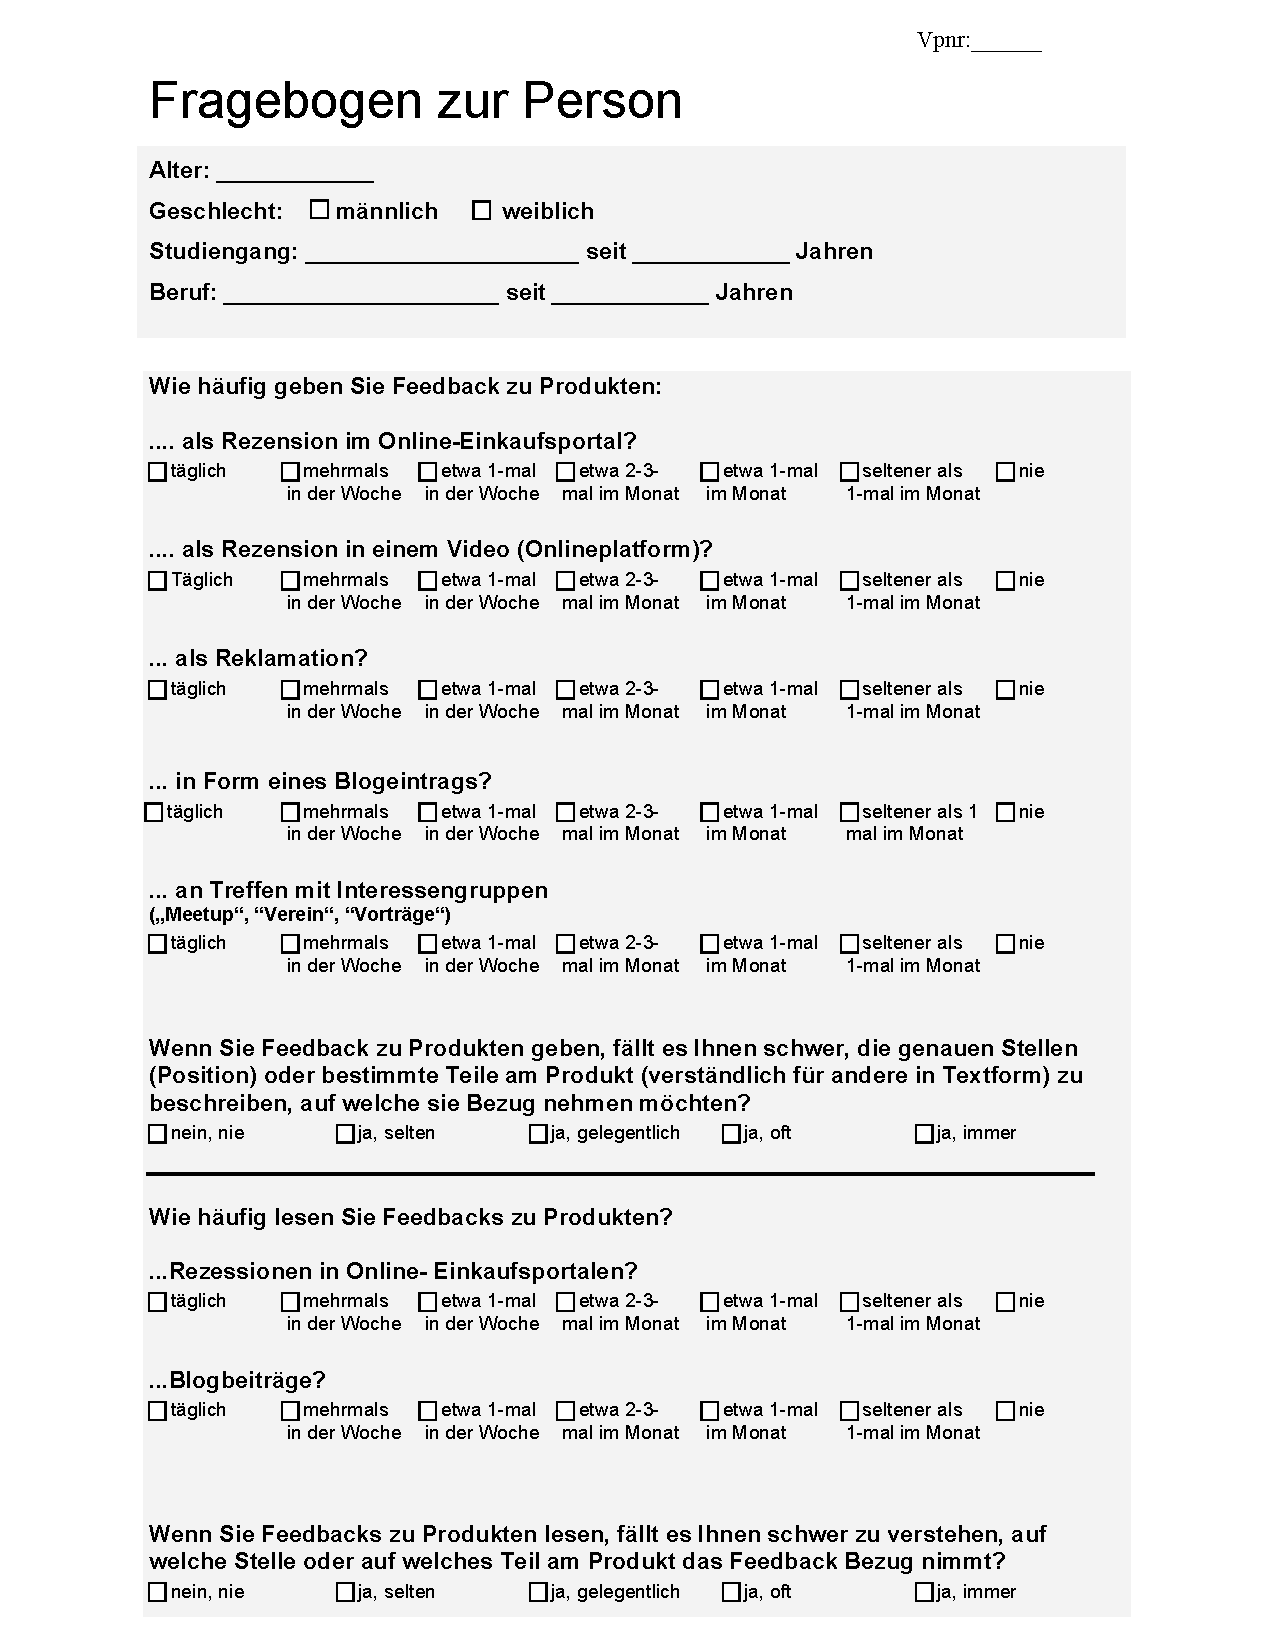
\includepdf[pages=-]{resources/anhang/Demografischer_Fragebogen.pdf}



% Eigenständigkeitserklärung
\addchap{Eigenständigkeitserklärung}

Hiermit versichere ich, dass ich die vorliegende Bachelorarbeit selbstständig und nur unter Verwendung der angegebenen Quellen und Hilfsmittel verfasst habe. Die Arbeit wurde bisher in gleicher oder ähnlicher Form keiner anderen Prüfungsbehörde vorgelegt.

\vskip 1cm

Berlin, den 09.09.2019

\vskip 1.5cm

Ali Bektas
 

\end{document}
